% !TEX root = ../thesis_main.tex
%
%
%
\clearpage
\appendix  
\addcontentsline{toc}{chapter}{Appendices}
%
%%%% --- * --- %%%%	
% !TEX root = ../thesis_main.tex
%
%
%
%%%% --- * --- %%%%	
\clearpage	
%\part{Appendices}
\chapter{Notable Differences in Data Selection between this and the Previous Result}
\label{ch:differences_data}
%\note[done]{Removed some appendices:
%\\
%- Very Obvious Things (on lifetimes and half-lifes) \\
%- On Beta Endpoint Energies ("notationandprelimintegration") \\
%- Wong Nuclear \\ 
%- HowTo Lifetime
%}

\note[jb1]{JB says Appendix A should all go in the analysis section, and not in an appendix at all.}
\note[jb1]{JB says:  Appendix A (ie, *this appendix*) is very important, and should at least be a subsection in the Analysis chapter.\\...\\You could condense the Appendix into a set of bullet points at the end of the intro​​ to the Analysis section (which you still need, badly!), and then its content could be interleaved in the Analysis chapter.  E.g. you already have redundancy in the LE and TE discussion vs. the Appendix, and the discussion is more complete in the Analysis chapter, which is good.  }
\note{I really want this appendix to stay here.  I'll make sure to mention everything in the body of the thesis though, since it *is* important.  But at some point, somebody is going to really want to have this info written into a short summary.}


\section{Polarization Cycle Selection}
	Data used for our recent PRL article was slightly less polarized than we thought it was, due to an oversight in the data selection procedure.  See Ch.~\ref{} for a discussion of the effects.
	
\section{Leading Edge / Trailing Edge and Walk Correction}
	%\\*
	Using the leading edge rather than the trailing edge to mark the timing of TDC pulses cleans up jitter, eliminates background, and changes the relative delays between different inputs.  It is immediately relevant to the shape of the `walk correction' on scintillator timing pulses, which give a different prediction for beta arrival time as a function of scintillator energy.  %This subsequently affects models for the fraction of background events.  
	
\section{TOF Cut + Background Modelling}
	A SOE-beta time-of-flight cut is necessary to reduce background.  The above mentioned walk correction directly results in an change in which specific events are selected in a given TOF cut.  It further results in an adjustment to the expected fraction of background events in any such cut.
	
%\section{BB1 Radius}
%	Possibly my default radius cut on the DSSDs is a bit different.  The region of the parameter space that I'm taking for the systematic uncertainty on this is definitely a bit different.  
	
\note{Somebody will surely ask for a justification for why I did this differently, and I don't have one beyond ``this seemed more reasonable to me", which is of course nobody will ever accept as a reason.}

\section{BB1 Energy Threshold}
	I use an overall 50 keV threshold, (taking +/- 10 keV from that as a systematic to be propagated/checked), but the collaboration's previous analysis used 60 keV as the default threshold.
%	I think Ben used 60 keV.  
	
% JB says:  disperse Appendix A to analysis section.
% !TEX root = ../thesis_main.tex



%%%% --- * --- %%%%	
\chapter[A PDF]{A PDF For The People}
\label{appendix_forthepeople}

\note[color=done]{John says to keep this appendix, because it's great now.}
%\note[color=jb]{JB:  Appendix B is in good shape. "someone other than me" please change to "the collaboration."}

\section[JTW]{JTW}
Here's a master equation from JTW to describe beta decay kinematics~\cite{jtw},~\cite{jtw_coulomb}:

% !TEX root = ../thesis_main.tex



% "A PDF for the People"
\bea
\omega(\cdots) \!\!\!\! \!\!\!\! \!\!\!\! \!\!\!\! && \,\,\,\, \,\,\,\, \mathrm{d} \E \, \dOmegae \, \dOmeganu 
\,\, = \,\, \frac{\FF}{(2\pi)^5} \, \pe \Ee (E_0 - \Ee)^2 \dEe \, \dOmegae \, \dOmeganu \, \nonumber\\ 
&&	\times \,\, \xi \left[
	1 + \a \frac{\vecpe\cdot\vecpnu}{\Ee\Enu} + \bFierz \frac{\m c^2}{\Ee} 
%	&& 
    + \,\,  \calign \,\, \Talign(\vecJ) 
	\left(
		\frac{\vecpe \cdot \vecpnu}{3\Ee\Enu}
		- \frac{ (\vecpe\cdot \hatj) (\vecpnu\cdot\hatj) }{\Ee\Enu}
	\right)
	\!
	%\left(
	%	\TalignExpand
	%\right)
\right. \nonumber\\ 
&&	\left. + 
	 \frac{\vecJ}{J} \cdot
	\left(
		\A \frac{\vecpe}{\Ee} 
		+ \B \frac{\vecpnu}{\Enu} 
		+ \D \frac{\vecpe \times \vecpnu}{\Ee\Enu} 
	\right)
\right]
\label{equation:jtw_master}
\eea

where, for convenience, we have defined a nuclear alignment term,
\bea
\Talign(\vecJ) &\equiv& \TalignExpand.
\eea
\aside{We have already specialized to $\beta^+$ decay.}

Note that this master equation depends on neutrino momentum, which we cannot observe directly.  Furthermore, we cannot reconstruct neutrino momenta in our decay events either, because it would be necessary to account for the momentum of the recoiling daughter nucleus, treating the decay as a three-body problem.  From an experimental standpoint, we failed to measure the momenta of the daughters in conjunction with the ``tagged'' beta decay events with which we are primarily concerned in this thesis.  From a theoretical standpoint, JTW has intentionally neglected recoil-order terms -- meaning that the daughter nucleus is treated, for the purpose of kinetic energy calculations, as being infinitely massive, and as such it must have no change in kinetic energy from the decay.  This approximation makes it a bit tricky to correctly re-formulate Eq.~(\ref{equation:jtw_master}) in terms of the momentum of the daughter instead of the momentum of the neutrino.  

Fortunately, it is possible to simplify Eq.~(\ref{equation:jtw_master}) by integrating over all possible neutrino directions, such that the result no longer depends on parameters that we do not observe.  The neutrino energy itself is not a free variable in this equation, because the energy release in the decay is fixed, and given the approximation that none of that energy is allocated to the recoiling daughter, it is very straightforward to calculate the neutrino energy for a decay event in which the beta energy is known.

%We haven't integrated out the neutrino momentum.  Neutrino energy itself is a redundant parameter, I think, because we are already using an endpoint energy and a beta energy, and we are not taking recoil-order effects into account.  Also, we treat neutrinos as massless here, which is a perfectly reasonable approximation for our purposes.  For ``convenience'', let's define a nuclear alignment term, $\Talign$, so that:


The result of performing this integration over neutrino direction is:
% !TEX root = ../thesis_main.tex
%
%
%
% The JTW Proto-Master
\bea
	\textrm{d}^3 \Gamma \dEe \, \dOmegae
	&=& 
	\frac{2}{(2\pi)^4} \, \FF \, \pe \Ee (E_0 - \Ee)^2 \, \dEe \, \dOmegae \, \xi \nonumber\\ 
	&& \times \left[
		1 + \bFierz \frac{\m c^2}{\Ee} + 
		\A  
		\left(
			\frac{\vecJ}{J} \cdot \frac{\vecpe}{\Ee} 
		\right) 
	\right],
\label{equation:integrated_jtw}
\eea
%\unskip which is a great simplification on Eq.~(\ref{equation:jtw_master}).  We still must write the remaining parameters in terms of the relevant nuclear matrix elements and fundamental coupling constants.  These coupling constants are, in general, complex-valued, and JTW does not choose a phase angle for us.  We write them out in 
Eqs.~(\ref{eq:jtw_xi}-\ref{eq:jtw_Abetaxi}).
% !TEX root = ../thesis_main.tex
%
%
%
%%%% --- * --- %%%%	
\begin{eqnarray}
    \xi &=& 
    	|M_F|^2    \left( |C_S|^2 + |C_V|^2 + |C_S^\prime|^2 + |C_V^\prime|^2 \right) 
		\nonumber \\ && + \;\; 
		|M_{GT}|^2 \left( |C_T|^2 + |C_A|^2 + |C_T^\prime|^2 + |C_A^\prime|^2 \right)
	\label{eq:jtw_xi} \\
    \bFierz \, \xi &=& \pm \: 2\gamma \, \textrm{Re}\!\left[ |M_F|^2 \left( C_S C_V^* + C_S^\prime C_V^{\prime *} \right) + |M_{GT}|^2 \left( C_T C_A^* + C_T^{\prime} C_A^{\prime *} \right) \right] 
    \label{eq:jtw_bxi} \\
    \Abeta \, \xi &=& |M_{GT}|^2 \lambda_{J^\prime J} \left[ \pm 2 \textrm{Re}\!\left[ C_T C_T^{\prime *} - C_A C_A^{\prime *} \right] + 2 \frac{\alpha Z \me }{\pbeta} \,\textrm{Im}\!\left[ C_T C_A^{\prime *} + C_T^\prime C_A^* \right] \right] 
		\nonumber \\ && + \;\; 
		\delta_{J^\prime J} \, |M_F| |M_{GT}| \left( \frac{J}{J+1} \right)^{\!\!\! 1/2} \left[ \phantom{\frac{1}{1}\!\!\!} 2 \,\textrm{Re} \! \left[ C_S C_T^{\prime *} +  C_S^\prime C_T^* - C_V C_A^{\prime *} - C_V^\prime C_A^* \right] 
		\right.
		\nonumber \\ && \pm \;\;
		\left.
		2 \frac{\alpha Z \me }{\pbeta} \,\textrm{Im}\!\left[ C_S C_A^{\prime *} + C_S^\prime C_A^* - C_V C_T^{\prime *} -C_V^\prime C_T^* \right] \right]
	\label{eq:jtw_Abetaxi}
\end{eqnarray}
%
%
Note that JTW presents slightly different expressions for the sign convention in components of $\Abeta$ within~\cite{jtw} and~\cite{jtw_coulomb}.  Here, we adopt the convention from the latter publication.  Furthermore, we do not require that either $M_F$ or $M_{GT}$ be positive (which would allow us to safely drop their absolute value indicators and make the conventions of these two papers equivalent).  In order to obtain the correct, physically observed value for $\Abeta$, we require that the 
$M_{F}\,M_{GT}$ term in Eq.~(\ref{eq:jtw_Abetaxi}) have an overall positive value.  Because we know that the scalar and tensor couplings must be small, and any imaginary contributions to the term must be small, we conclude that
\bea
	M_{F}\,M_{GT} \left( C_V C_A^{\prime *} + C_V^\prime C_A^* \right) < 0.
\eea

%\note{In order to make JTW give us the correct, physically observed value for $\Abeta$, we need ... something.  JTW writes an expression for $\Abeta$ with slightly different sign convention in~\cite{jtw} and~\cite{jtw_coulomb}.  There is some subtlety involved in getting the correct signs on things, but the easiest way to figure it out is to make sure the calculation of the value of $\Abeta$ matches reality.  To this end, ... either for both $M_{GT}$ and $M_{F}$ to be positive, or we use the notation for $\Abeta$ from JTW's earlier paper rather than the one with the coulomb corrections.  Somehow, we run into problems getting JTW to agree with Holstein if we require $M_{GT}$ and $M_{F}$ to have the same sign, so we're going to kludge together two different expressions for $\Abeta$ from both of JTW's papers.  Or ... wait ... maybe the opposite thing is what I should be doing?  In handwritten notes, I explicitly use the *later* JTW sign convention.}

%\note{In order to make JTW give us the correct, physically observed value for $\Abeta$, we need either for both $M_{GT}$ and $M_{F}$ to be positive, or we use the notation for $\Abeta$ from JTW's earlier paper rather than the one with the coulomb corrections.  Somehow, we run into problems getting JTW to agree with Holstein if we require $M_{GT}$ and $M_{F}$ to have the same sign, so we're going to kludge together two different expressions for $\Abeta$ from both of JTW's papers.  Or ... wait ... maybe the opposite thing is what I should be doing?  In handwritten notes, I explicitly use the *later* JTW sign convention.}

\aside{Also, $\xi = G_v^2 \, \cos\theta_C \, f_1(E).$}


\section[Holstein]{Holstein} 
Holstein~\cite{holstein}~\cite{holstein_errata} generously provides explicit equations to match both Eq.~(\ref{equation:jtw_master}) (i.e. Holstein's Eq.~(51), where neutrino direction is a parameter of the probability distribution) and Eq.~(\ref{equation:integrated_jtw}) (Holstein's Eq.~(52), where neutrino direction has already been integrated over).  

%Holstein~\cite{holstein} generously provides explicit equations to match both Eq.~\ref{equation:jtw_master} (where neutrino direction is a parameter of the probability distribution), and Eq.~\ref{equation:integrated_jtw} (where the neutrino direction has already been integrated over).

%This one is harder.  But here, we've already integrated over neutrino momentum at least.  That's something.  

Here's Holstein's Eq.~(52):
% !TEX root = ../thesis_main.tex



% "A PDF for the People"
\bea
\mathrm{d}^3 \Gamma &=& 2  G_v^2 \cos^2\theta_c \frac{\FF}{(2\pi)^4} \, \pe \Ee (E_0 - \Ee)^2 \dEe \, \dOmegae 
\nonumber\\
&& \times
\left\{
	F_0(\E) 
	+ \Lambda_1 F_1(\E) \hatn \cdot \frac{\vecpe}{\Ee}
	+ \Lambda_2 F_2(\E) \left[ \left( \nhat \cdot \frac{\vecpe}{\Ee} \right)^2 - \frac{1}{3}\frac{\pe^2}{\Ee^2} \right]
	\right. \nonumber\\ && \left.
	+ \Lambda_3 F_3(\E) 
		\left[ 
			\left( \hatn \cdot \frac{\vecpe}{\Ee} \right)^3
			- \frac{3}{5}\frac{\pe^2}{\Ee^2}\hatn \cdot \frac{\vecpe}{\Ee}
		\right]
\right\}
\label{equation:holstein52}
\eea
\unskip

A careful reader will eventually note that Holstein's spectral functions $F_i(\Ee)$ are not the same as the $F_i(\Ee, u, v, s)$ in any limit, despite the notational similarities.  Among other rules, Holstein's spectral functions obey these:
\bea
	F_i(\Ee) &\neq& F_i(\Ee, u, v, s)    \\
	F_i(\Ee) &=&    H_i(\Ee, u, v, 0)    \\
	f_i(\Ee) &=&    F_i(\Ee, u, v, 0).
\eea
For the $F_i(\Ee)$ functions of interest to us here, we find the following relationships:
%though expressions for $F_i(\Ee)$ can still be obtained through a chain of substitutions: 
\begin{align}
F_0(\Ee) & = H_0(\Ee, J, J^\prime, 0) = F_1(\Ee, J, J^\prime, 0) 
	\!\!\! 
	& = &\; f_1(\Ee) 
	\nonumber \\
F_1(\Ee) & = H_1(\Ee, J, J^\prime, 0) = \textstyle F_4(\Ee, J, J^\prime, 0) \,+\! \frac{1}{3}F_7(\Ee, J, J^\prime, 0) 
	\!\!\! 
	& = &\; \textstyle f_4(\Ee) \,+\! \frac{1}{3}f_7(\Ee) 
	\nonumber \\
F_2(\Ee) & = H_2(\Ee, J, J^\prime, 0) = \textstyle F_{10}(\Ee, J, J^\prime, 0) \!+\! \frac{1}{2}F_{13}(\Ee, J, J^\prime, 0) 
	\!\!\! 
	& = &\; \textstyle f_{10}(\Ee) \!+\! \frac{1}{3}f_{13}(\Ee) 
	\nonumber \\
F_3(\Ee) & = H_3(\Ee, J, J^\prime, 0) = F_{18}(\Ee, J, J^\prime, 0) 
	\!\!\!
	& = &\; f_{18}(\Ee) .
\label{eq:holstein_FHFf}
\end{align}
\unskip  % eq:holstein_FHFf

Note that the $f_i(\Ee)$ in Eq.~\ref{eq:holstein_FHFf} are the same spectral functions used to describe a polarized decay spectrum when the neutrino (ie, the recoil) is also observed -- though of course such a spectrum must have other terms as well.  For the spectrum of interest to us here, in which the neutrino direction has already been integrated over, we can simply look up the $H_i(\Ee, J, J^\prime, 0) = H_i(E, u, v, s\!=\!0)$ spectral functions, and leave it at that.  We find:
%Here, we've taken $u=J$ and $v=J^\prime$ to be the initial and final angular momenta respectively, because apparently I'm having a hard time keeping my notation straight.
% !TEX root = ../thesis_main.tex
%
%
%
%%%% --- * --- %%%%	
\begin{multline}
F_0(\Ee) = 
\left| a_1 \right|^2 
+ 2 \Re\left[ a_1^* a_2 \right] \frac{1}{3 M^2} 
\left[  
	\m^2 + 4 \Ee E_0 + 2 \frac{\me^2}{\Ee}E_0 - 4\Ee^2
\right]
\\
+ \left| c_1 \right|^2
+ 2 \Re\left[ c_1^* c_2\right] \frac{1}{9 M^2} 
\left[
	11 \me^2 + 20 \Ee E_0 
	- 2\frac{\me^2}{\Ee}E_0
	- 20\Ee^2
\right]
- 2 \frac{E_0}{3M} \Re\left[ c_1^*(c_1 + d \pm b)\right]
\\
+ \frac{2\Ee}{3M} 
\left( 
	3 \left| a_1 \right|^2 + \Re \left[ c_1^*(5c_1 \pm 2 b) \right]
\right)
- \frac{\me^2}{3 M \Ee} 
\Re \left[ 
	-3 a_1^*e + c_1^*\left(2c_1 + d \pm 2b - h\frac{E_0 - \Ee}{2M} \right)
\right]
\end{multline}
%\unskip
% !TEX root = ../thesis_main.tex
%
%
%
%%%% --- * --- %%%%	
\begin{align}
F_1(\Ee) = & \:\:
\deltauv \left( \frac{u}{\!u+1\!} \right)^{\!\!1/2} \!\!
\left\{
	2 \Re\left[ 
		a_1^*\left(\! c_1 - \frac{E_0}{3M}(c_1 + d \pm b) + \frac{\Ee}{3M}( 7 c_1 \pm b + d )\! \right)
	\right]
	\right. \nonumber \\ & \left. 
	+
	2 \Re\left[
		a_1^* c_2 + c_1^* a_2
	\right] \!
	\left(
		\frac{4 \E(E_0 - \E) + 3 \me^2}{3M^2}
	\right) \!
\right\}
\nonumber \\ &
\mp \frac{ (-1)^s \gammauv}{u+1} 
\Re \left\{ \!
	c_1^* \! \left(
		c_1 + 2 c_2 \left(\frac{8\Ee(E_0-\Ee)+3\me^2}{3M^2}\right)
		- \frac{2 E_0}{3 M} (c_1 + d \pm b) 
		\right.\right. \nonumber \\ & \left.\left.
		+ \frac{\Ee}{3M} (11 c_1 - d \pm 5 b)
	\right)
\right\}
%\nonumber \\ &
+ 
\frac{\lambdauv}{u+1}
\Re \left\{ \!
	c_1^* \! \left[
		- f \left(\frac{5\Ee}{M}\right)
		\right. \right. \nonumber \\ & \left. \left.
		+ g \left( \frac{3}{2} \right)^{\!\!1/2} \!
		\left(
			\frac{E_0^2 - 11 E_0 \Ee + 6 \me^2 + 4\Ee^2 }{6M^2}
		\right) 
		%\right.\right. \nonumber \\ & \left.\left.
		\pm 3 j_2 
		\left(
			\frac{8 \Ee^2 - 5E_0 \Ee - 3 \me^2}{6M^2}
		\right)
	\right] \!
\right\}
\end{align}
%\unskip
% !TEX root = ../thesis_main.tex
%
%
%
%%%% --- * --- %%%%	
\begin{flalign}
F_2(\Ee) = &
\thetauv \frac{\Ee}{2M} 
\Re\left[
	c_1^*\left(
		c_1 + c_2 \frac{8(E_0-\Ee)}{3M}
		-d \pm b
	\right)
\right]
&& \nonumber \\ &
- \deltauv \frac{\Ee}{M} 
\left[ \frac{u(u+1)}{(2u-1)(2u+3)} \right]^{1/2} \!
\Re \left\{ \!
	a_1^*\left( 
		\left( \! \frac{3}{2} \right)^{\!\!1/2}\!\! f
		+ g \frac{\Ee+2E_0}{4M} 
		\right.\right.
		&& \nonumber \\ &
		\left.\left.
		\pm \left( \frac{3}{2} \right)^{\!\!1/2}\!\! j_2 \frac{E_0-\E}{2M}
	\right) \!
\right\}
+ (-1)^s \, \kappauv \frac{\E}{2M}
\Re \left[
	c_1^* \! \left(
		\pm \, 3 f 
		\pm \left( \frac{3}{2} \right)^{\!\!1/2}\!\! g \frac{E_0-\Ee}{M}
		\right.\right.
		&& \nonumber \\ &
		\left.\left.
		+ 3 j_2 \frac{E_0-2\Ee}{2M}
	\right)
\right]
+ \epsilonuv \Re\left[ c_1^* j_3 \right]
\left( 
	\frac{21 \E^2}{8 M^2}
\right) &&
\end{flalign}
%\unskip
% !TEX root = ../thesis_main.tex
%
%
%
%%%% --- * --- %%%%	
\begin{flalign}
F_3(\Ee) = &
- \deltauv \, (3 u^2 + 3 u -1)
\left[
	\frac{u}{(u-1)(u+1)(u+2)(2u-1)(2u+3)}
\right]^{1/2}\!
&& \nonumber \\ &
\times 
\Re \left[
	a_1^* j_3
\right]
\left( 
	\frac{\Ee^2 \sqrt{15} }{4M^2}
\right)
+ 
\frac{\rhouv}{u+1} 
\Re \left[
	c_1^*(g\sqrt{3} + j_2\sqrt{2})
	\left(
		\frac{5 \Ee^2}{4 M^2}
	\right)
\right]
&& \nonumber \\ &
\pm
\frac{(-1)^s \sigmauv }{u+1} 
\Re \left[ c_1^*j_3 \right] 
\left( 
	\frac{5\Ee^2}{2 M^2}
\right) &&
\label{equation:holstein_F3}
\end{flalign}
%\unskip
and we might really appreciate if these things could be simplified a bit.  

The terms $a_1, a_2, b, c_1, c_2, d, e, f, g, h, j_2, j_3$ are ``structure functions''.  Holstein gives some predictions for their form, assuming the impulse approximation holds, in his Eq.~(67). \aside{There was something wrong with this assumption.  Something circular.  I forget.  Blah.}  For the most part, the values and form of these structure functions are beyond the scope of this thesis, so I will not re-write them all here. 
%\aside{Or will I?}  
It should be noted that the numerical values used for these parameters came from a private communication from Ian Towner to the collaboration.
%\comment{It should be noted that the numerical values used for these parameters came from a private communication from Ian Towner to ... someone other than me.}  
However, it is important to note the expressions for $a_i$ and $c_i$, because these will directly come into play when we try to reconcile Holstein's expression with JTW's.  Therefore, 
\bea
a(q^2) &\approx& \frac{g_V(q^2)}{(1 + \frac{\Delta}{2M})} \left[ M_F    + \frac{1}{6}(q^2 - \Delta^2) M_{r^2} + \frac{1}{3} \Delta M_{\mathbf{r} \cdot \mathbf{p} } \right] 
\label{equation:full_a}
\\ 
c(q^2) &\approx& \frac{g_A(q^2)}{(1 + \frac{\Delta}{2M})} \left[ M_{GT} + \frac{1}{6}(q^2 - \Delta^2) M_{\sigma r^2} + \frac{1}{6 \sqrt{10} }(2\Delta^2 + q^2) M_{1y} 
\right. \nonumber \\ && \left.
+ A \frac{\Delta}{2 M} M_{\sigma L} + \frac{1}{2} \Delta M_{\sigma r p} \right]
\label{equation:full_c}
\eea
\note{Somewhere I have to define $q^2$ and $\Delta$ are.}
...where the $M_{xxx}$'s are certain nuclear matrix elements.  \aside{Should I just list the values of things that I inherited from Ian Towner's personal communication that one time?}  However, Eqs.~(\ref{equation:holstein_F0}-\ref{equation:holstein_F3}) are not written in terms of $a(q^2)$ and $c(q^2)$, but rather in terms of $a_1$, $a_2$, $c_1$, and $c_2$.  In fact, Holstein is implicitly using series expansions to remove the dependence on recoil momentum, so that
\bea
a(q^2) &=& a_1 + \left(\! \frac{q^2}{M^2} \! \right) a_2 + \cdots \label{equation:series_expand_a} \\
c(q^2) &=& c_1 + \left(\! \frac{q^2}{M^2} \! \right) c_2 + \cdots \label{equation:series_expand_c}
\eea

%Also, Holstein proceeds to split up $a(q^2)$ and $c(q^2)$ into their first two Taylor series terms for an expansion of .... $q/M$, maybe?  Or possibly $q^2 / M^2$?  Anyway, that's $a_1$ and $a_2$, and $c_1$ and $c_2$, in Holstein notation.  He doesn't do that with any of the other structure functions. 
%\bluetodo{Seriously, I need to check what the taylor series is even expanding in.}


%\note{In fact, we might want to add the other different-er terms in to this thing now, before we get ahead of ourselves.}
Next, Holstein goes and tweaks those $F_i(\Ebeta)$ terms that we've already written out, by adding in an adjustment for Coulomb corrections.  Those corrections have this form:
\beq
	F_i(\Ebeta) \rightarrow \tilde{F}_i(\Ebeta) := \FF \left[ F_i(\Ebeta) + \Delta F_i(\Ebeta) \right]
\eeq

To obtain expressions for the $\Delta F_i(\Ebeta)$, Holstein invokes some Feynman diagrams and provides expressions for several integrals, all of which are both complex and complicated.  The modified spectral functions are provided in terms of functions of these integrals.  Since nobody wants to have to evaluate those integrals, Holstein makes a further approximation by taking only the first term in an expansion of the $\Delta F_i(\Ebeta)$ in terms of $Z\alpha$, where $Z\alpha \ll 1$.  Then, the resulting expressions for $\Delta F_i(\Ebeta)$ can be written in terms of much more straightforward integrals over form factors for electric change and weak charge.  

If we make the further assumption that these form factors are identical, and that both types of charge are spread over a ball of uniform density with radius $R$,\aside{and also, I think something like that the weak charge is the same distribution as the electric charge} then we find:
\bea
	X = Y = \frac{9\pi R}{140}
\eea
in the Eqs.~(\ref{eq:holstein_DeltaF1_Euvs} - \ref{eq:holstein_DeltaF7_Euvs}) that follow.

Because Holstein doesn't actually write this stuff out in terms of $F_i(\Ebeta)$, but rather in terms of $F_i(\Ebeta, u,v,s)$, this correction presents yet another opportunity for the reader to interpret his notation incorrectly.  We note that one must remember to make use of the relations in Eq.~(\ref{eq:holstein_FHFf}).  Furthermore, Holstein notes that some of the terms $F_i(\Ebeta, u,v,s)$ are suppressed already, and he does not consider those terms further.  We will take this approximation to be adequate for our purposes here.

%\note{So clearly I'm going to need terms for $\Delta F_1(\Ebeta, u, v, s)$, $\Delta F_4(\Ebeta, u, v, s)$, $\Delta F_7(\Ebeta, u, v, s)$, $\Delta F_{10}(\Ebeta, u, v, s)$, $\Delta F_{13}(\Ebeta, u, v, s)$, and $\Delta F_{18}(\Ebeta, u, v, s)$. We really only have expressions for some of them in Holstein's Eq.~(C4).  In particular, we've got $\Delta F_1(\Ebeta, u, v, s)$, $\Delta F_4(\Ebeta, u, v, s)$ and $\Delta F_7(\Ebeta, u, v, s)$, but we're missing $\Delta F_{10}(\Ebeta, u, v, s)$, $\Delta F_{13}(\Ebeta, u, v, s)$, and $\Delta F_{18}(\Ebeta, u, v, s)$.  That's annoying.  Holstein gives as an excuse for that (have to check to make sure it works and that it's actually an excuse is for this) that the recoil terms $b$, $d$, and $f$ are already suppressed in their contribution to beta decay spectra. }

\note{ What is less clear, given the context in the paper, is whether or not when Holstein writes out his simplified expressions for $\Delta F_{x}(\Ebeta, u, v, s)$ he actually means $ \FF \Delta F_{i}(\Ebeta, u, v, s)$.  These terms are pretty small, so it probably doesn't *really* matter, but it would still be really nice to *know*, damn it.}

So, we'll write out the functions for these corrections.  
% !TEX root = ../thesis_main.tex
%
%
%
%%%% --- * --- %%%%	
\begin{flalign}
\Delta F_1(\Ee, u, v, s) = &
\mp \left( \frac{8 \alpha Z}{3\pi } \right) \left\{ |a|^2 \left[ 4 \Ee (X+Y) + E_0 X + \textstyle{\frac{\m c^2}{\Ee }}(X+2Y) \right] 
\right. &&\nonumber \\ & \left.
+ |c|^2\left[ \Ee ( \textstyle{\frac{16}{3}} X + 4 Y)  - \textstyle{\frac{1}{3}}E_0 X + \textstyle{\frac{\m c^2}{\Ee }} (X+2Y) \right]
\right\} &&
\label{eq:holstein_DeltaF1_Euvs}
\end{flalign}
% 
% 
% 
% \textstyle{\frac{16}{3}}\unskip
% !TEX root = ../thesis_main.tex
%
%
%
%%%% --- * --- %%%%	
\begin{flalign}
\Delta F_4(\Ee, u, v, s) = &
\mp \left( \frac{8 \alpha Z}{3\pi } \right) \Ee \, (5X + 4Y) \left[ \deltauv \left( \frac{u}{u+1} \right)^{1/2} 2\Re \,[a^* c] 
\right. && \nonumber \\ & \left.
\mp (-1)^s \left( \frac{\gammauv}{u+1} \right)^{\phantom{1/2}}\!\!\!\!\! |c|^2 \right] 
&&
\end{flalign}
% 
% 
% 
% \textstyle{\frac{16}{3}}\unskip
% !TEX root = ../thesis_main.tex
%
%
%
%%%% --- * --- %%%%	
\begin{align}
\Delta F_7(\Ee, u, v, s) = &
\mp \left( \frac{8 \alpha Z}{3\pi } \right) \left[ \deltauv \left( \frac{u}{u+1} \right)^{1/2} 2\Re \,[a^* c] 
\right. \nonumber \\ & \left.
\mp (-1)^s \left( \frac{\gammauv}{u+1} \right)^{\phantom{1/2}}\!\!\!\!\! |c|^2 \right] (E_0 - \Ee) X
\label{eq:holstein_DeltaF7_Euvs}
\end{align}
% 
% 
% 
% \textstyle{\frac{16}{3}}\unskip

We note that the above corrections have been written in terms of $a(q^2)$ and $c(q^2)$, and we must use Eqs.~(\ref{equation:series_expand_a}, \ref{equation:series_expand_c}) to put the results in terms of $a_1$,  $a_2$, $c_1$, and $c_2$ so that they can be correctly combined with Eqs.~(\ref{equation:holstein_F0}-\ref{equation:holstein_F3}).

If we evaluate Holstein's Eqs.~(B8), which I will absolutely not type out here, for the case $u=v=J=J^\prime=3/2$, we find the following values:
\begin{align}
\deltauv     &= 1 
& \thetauv   &= 1 
& \rhouv     &= \frac{-41}{40}
	\nonumber\\
\gammauv     &= 1 
& \kappauv   &=\frac{1}{2\sqrt{2}} % \;\; ! \!=\;\; \frac{3}{\sqrt{2}}
& \sigmauv   &= \frac{-41}{4\sqrt{35}}
	\nonumber\\
\lambdauv    &= \frac{-\sqrt{2} }{5} % 2\sqrt{3} 
& \epsilonuv &= \frac{-1}{2\sqrt{5}}
& \phiuv     &= 0 % \frac{1}{32} \left(\frac{3}{5}\right)^{\!1/2}.
	\nonumber\\
\label{eq:holstein_greekletterfunctions}
%
\end{align}
\unskip  % eq:holstein_greekletterfunctions
Furthermore, in our calculations here, we will be considering only the $\beta^+$ decay modes, and therefore we take the \emph{lower} sign when the option arises.  We also will use $s=0$, so that $(-1)^s = +1$.
\note{Also, pretty sure one of those never gets used.  Which one was it?  idk.}


%%% -- %%%
- -- --- -- - 

Let's define some of that notation!
Firstly, 
\bea
\textrm{Holstein's \,} \hat{n} &=& \textrm{JTW's \,} \mathbf{j},
\label{eq:nequalsj}
\eea
and the 
$\Lambda_i$ are given by Holstein's Eq.~(48):
\bea
    \Lambda_1   &:=& \LambdaOne   
    \label{eq:lambda1} \\
    \Lambda_2   &:=& \LambdaTwo 
    \label{eq:lambda2} \\
    \Lambda_3   &:=& \LambdaThree .
    \label{eq:lambda3}
\eea

\aside{Note:  It's not the case that $ | \vecJ | == J $.  It's actually super fucking infuriating notation. }

We immediately see that Holstein's $\Lambda_1$ is closely related to JTW's $\frac{\vecJ}{J}$, and a bit later after John points it out to us, we see that Holstein's $\Lambda_2$ is closely related to JTW's $\Talign$.  JTW doesn't have any equivalent to $\Lambda_3$.  In particular, we find:
\bea
\Lambda_1 \hatj &=& \LambdaOne \hatj \;\; = \;\; \frac{\vecJ}{J}  \\
%\Lambda_2 \frac{(J+1)}{(2J-1)} &=& \Talign
\Lambda_2 &=& \Talign \frac{(2J-1)}{(J+1)}.
\eea


%Now we'll have to deal with expanding the $F_i(\Ee)$.  %Note that these are very different from the $F_i(\Ee, u, v, s)$, and also different from the $f_i(\Ee)$.  
%Holstein makes a goddamn mess of this, so here we go!  From Holstein's Eq.~(B10):
%\bea
%F_i(\Ee) &=& H_i(\Ee, J, J^\prime, 0).
%\eea
%%and from Holstein's Eq.~(B9), we see that 
%%\bea
%%f_i(\Ee) &=& F_i(\Ee, J, J^\prime, 0)
%%\eea
%From Holstein's many Eqs.~(B7), we see that the $H_i(\Ee, u, v, s)$ can be written in terms of the functions $F_i(\Ee, u, v, s)$, which we carefully note \emph{are not the same} as the functions $F_i(\Ee)$.  We further see, from Holstein's Eq.~(B9) that a further set of functions, $f_i(\Ee)$ are defined in terms of the $F_i(\Ee, u, v, s)$.  In particular, Holstein's Eq.~(B9) states that
%\bea
%f_i(\Ee) &=& F_i(\Ee, J, J^\prime, 0).
%\eea
%Then, if we combine (some parts of) Holstein's Eqs.~(B7) with (B9) and (B10):
%\begin{align}
F_0(\Ee) & = H_0(\Ee, J, J^\prime, 0) = F_1(\Ee, J, J^\prime, 0) 
	\!\!\! 
	& = &\; f_1(\Ee) 
	\nonumber \\
F_1(\Ee) & = H_1(\Ee, J, J^\prime, 0) = \textstyle F_4(\Ee, J, J^\prime, 0) \,+\! \frac{1}{3}F_7(\Ee, J, J^\prime, 0) 
	\!\!\! 
	& = &\; \textstyle f_4(\Ee) \,+\! \frac{1}{3}f_7(\Ee) 
	\nonumber \\
F_2(\Ee) & = H_2(\Ee, J, J^\prime, 0) = \textstyle F_{10}(\Ee, J, J^\prime, 0) \!+\! \frac{1}{2}F_{13}(\Ee, J, J^\prime, 0) 
	\!\!\! 
	& = &\; \textstyle f_{10}(\Ee) \!+\! \frac{1}{3}f_{13}(\Ee) 
	\nonumber \\
F_3(\Ee) & = H_3(\Ee, J, J^\prime, 0) = F_{18}(\Ee, J, J^\prime, 0) 
	\!\!\!
	& = &\; f_{18}(\Ee) .
\label{eq:holstein_FHFf}
\end{align}
\unskip
%So that's fun.  Note that the $f_i(\Ee)$ are what goes into the polarized decay spectrum when the neutrino (ie, the recoil) is also observed.  It's a more complicated spectrum that way.  For this spectrum in which the neutrino has already been integrated over, we can just look up the $H_i(\Ee, J, J^\prime, 0) = H_i(\Ee, u, v, s)$ spectral functions, and leave it at that.
%So let's do this thing!
%% !TEX root = ../thesis_main.tex
%
%
%
%%%% --- * --- %%%%	
\begin{multline}
F_0(\Ee) = 
\left| a_1 \right|^2 
+ 2 \Re\left[ a_1^* a_2 \right] \frac{1}{3 M^2} 
\left[  
	\m^2 + 4 \Ee E_0 + 2 \frac{\me^2}{\Ee}E_0 - 4\Ee^2
\right]
\\
+ \left| c_1 \right|^2
+ 2 \Re\left[ c_1^* c_2\right] \frac{1}{9 M^2} 
\left[
	11 \me^2 + 20 \Ee E_0 
	- 2\frac{\me^2}{\Ee}E_0
	- 20\Ee^2
\right]
- 2 \frac{E_0}{3M} \Re\left[ c_1^*(c_1 + d \pm b)\right]
\\
+ \frac{2\Ee}{3M} 
\left( 
	3 \left| a_1 \right|^2 + \Re \left[ c_1^*(5c_1 \pm 2 b) \right]
\right)
- \frac{\me^2}{3 M \Ee} 
\Re \left[ 
	-3 a_1^*e + c_1^*\left(2c_1 + d \pm 2b - h\frac{E_0 - \Ee}{2M} \right)
\right]
\end{multline}
%\unskip
%% !TEX root = ../thesis_main.tex
%
%
%
%%%% --- * --- %%%%	
\begin{align}
F_1(\Ee) = & \:\:
\deltauv \left( \frac{u}{\!u+1\!} \right)^{\!\!1/2} \!\!
\left\{
	2 \Re\left[ 
		a_1^*\left(\! c_1 - \frac{E_0}{3M}(c_1 + d \pm b) + \frac{\Ee}{3M}( 7 c_1 \pm b + d )\! \right)
	\right]
	\right. \nonumber \\ & \left. 
	+
	2 \Re\left[
		a_1^* c_2 + c_1^* a_2
	\right] \!
	\left(
		\frac{4 \E(E_0 - \E) + 3 \me^2}{3M^2}
	\right) \!
\right\}
\nonumber \\ &
\mp \frac{ (-1)^s \gammauv}{u+1} 
\Re \left\{ \!
	c_1^* \! \left(
		c_1 + 2 c_2 \left(\frac{8\Ee(E_0-\Ee)+3\me^2}{3M^2}\right)
		- \frac{2 E_0}{3 M} (c_1 + d \pm b) 
		\right.\right. \nonumber \\ & \left.\left.
		+ \frac{\Ee}{3M} (11 c_1 - d \pm 5 b)
	\right)
\right\}
%\nonumber \\ &
+ 
\frac{\lambdauv}{u+1}
\Re \left\{ \!
	c_1^* \! \left[
		- f \left(\frac{5\Ee}{M}\right)
		\right. \right. \nonumber \\ & \left. \left.
		+ g \left( \frac{3}{2} \right)^{\!\!1/2} \!
		\left(
			\frac{E_0^2 - 11 E_0 \Ee + 6 \me^2 + 4\Ee^2 }{6M^2}
		\right) 
		%\right.\right. \nonumber \\ & \left.\left.
		\pm 3 j_2 
		\left(
			\frac{8 \Ee^2 - 5E_0 \Ee - 3 \me^2}{6M^2}
		\right)
	\right] \!
\right\}
\end{align}
%\unskip
%% !TEX root = ../thesis_main.tex
%
%
%
%%%% --- * --- %%%%	
\begin{flalign}
F_2(\Ee) = &
\thetauv \frac{\Ee}{2M} 
\Re\left[
	c_1^*\left(
		c_1 + c_2 \frac{8(E_0-\Ee)}{3M}
		-d \pm b
	\right)
\right]
&& \nonumber \\ &
- \deltauv \frac{\Ee}{M} 
\left[ \frac{u(u+1)}{(2u-1)(2u+3)} \right]^{1/2} \!
\Re \left\{ \!
	a_1^*\left( 
		\left( \! \frac{3}{2} \right)^{\!\!1/2}\!\! f
		+ g \frac{\Ee+2E_0}{4M} 
		\right.\right.
		&& \nonumber \\ &
		\left.\left.
		\pm \left( \frac{3}{2} \right)^{\!\!1/2}\!\! j_2 \frac{E_0-\E}{2M}
	\right) \!
\right\}
+ (-1)^s \, \kappauv \frac{\E}{2M}
\Re \left[
	c_1^* \! \left(
		\pm \, 3 f 
		\pm \left( \frac{3}{2} \right)^{\!\!1/2}\!\! g \frac{E_0-\Ee}{M}
		\right.\right.
		&& \nonumber \\ &
		\left.\left.
		+ 3 j_2 \frac{E_0-2\Ee}{2M}
	\right)
\right]
+ \epsilonuv \Re\left[ c_1^* j_3 \right]
\left( 
	\frac{21 \E^2}{8 M^2}
\right) &&
\end{flalign}
%\unskip
%% !TEX root = ../thesis_main.tex
%
%
%
%%%% --- * --- %%%%	
\begin{flalign}
F_3(\Ee) = &
- \deltauv \, (3 u^2 + 3 u -1)
\left[
	\frac{u}{(u-1)(u+1)(u+2)(2u-1)(2u+3)}
\right]^{1/2}\!
&& \nonumber \\ &
\times 
\Re \left[
	a_1^* j_3
\right]
\left( 
	\frac{\Ee^2 \sqrt{15} }{4M^2}
\right)
+ 
\frac{\rhouv}{u+1} 
\Re \left[
	c_1^*(g\sqrt{3} + j_2\sqrt{2})
	\left(
		\frac{5 \Ee^2}{4 M^2}
	\right)
\right]
&& \nonumber \\ &
\pm
\frac{(-1)^s \sigmauv }{u+1} 
\Re \left[ c_1^*j_3 \right] 
\left( 
	\frac{5\Ee^2}{2 M^2}
\right) &&
\label{equation:holstein_F3}
\end{flalign}
%\unskip
%...Phew!  I typed all of that out just so that I can have a record of what's going on here, but actually, the very first thing I want to do is make some simplifications here.  


% %%%%%%%%%%%%%%%%%%%%%%%%%%%%%% 
% \subsubsection[Algebra]{Algebra}
% Oookay.  Here's some stuff I'll want to keep track of now, but will also want to not have cluttering my documents later.
% \begin{align}
% \deltauv \left( \frac{u}{u+1} \right)^{\!\!1/2} \;\;&=\;\; \left( \frac{3}{5} \right)^{1/2}
% \\
% \mp \frac{ (-1)^s \gammauv}{u+1} \;\;&=\;\; \frac{2}{5}
% \\
% \frac{\lambdauv}{u+1} \;\;&=\;\; \frac{4 \sqrt{3}}{5}
% \\
% - \deltauv \left[ \frac{u(u+1)}{(2u-1)(2u+3)} \right]^{1/2}  \;\;&=\;\;  \frac{-\sqrt{5}}{4}
% \\
% %(-1)^s \kappauv \;\;&=\;\; \frac{3}{\sqrt{2}}  % I math-ed this wrong before.  I think.
% (-1)^s \kappauv \;\;&=\;\; \frac{1}{2\sqrt{2}}
% \\
% \frac{21}{8} \epsilonuv \;\;&=\;\; \frac{-21}{16 \sqrt{35}} %\;\;=\;\;
% \\
% \!\!\!\! \!\!\!
% - \deltauv (3 u^2 + 3 u -1)
% \left[
% 	\frac{u}{(u-1)(u+1)(u+2)(2u-1)(2u+3)}
% \right]^{1/2}\!
% \left(
% 	\frac{\sqrt{15}}{4}
% \right)
% \;\;&=\;\; \frac{-41 \sqrt{3}}{16 \sqrt{7}}
% \\
% \frac{\rhouv}{u+1}\left( \frac{5}{4} \right) \;\;&=\;\; \frac{41}{80}
% \\
% \pm
% \frac{(-1)^s \sigmauv }{u+1} \left( \frac{5}{2} \right) \;\;&=\;\; \frac{-41}{4\sqrt{35}}
% \end{align}
% %%%%%%%%%%%% Probably check the math on all of these over again.
% Note:  I calculated $\kappa_{u,v}$ wrong before.  Probably.  Unclear about the order of operations in really old papers.
%
% \subsubsection[More Algebra]{More Algebra}
% So here are some simplifications, using those expressions we just calculated in the stupid section above.
% %
% \begin{multline}
% F_0(\Ee) =
%   \left| a_1 \right|^2
% + \left( \!
% 	\frac{2\Ee}{M}
% \! \right)
% \left| a_1 \right|^2
% + \left| c_1 \right|^2
% + \left( \!
% 	\frac{- 2 E_0 + 10\Ee - 2\me^2/\Ee}{3M}
% \! \right)
% \left| c_1 \right|^2
% \\
% %
% + \frac{\me^2}{3 M \Ee}
% \left(
% 	3 Re\left[a_1^*e\right] - Re\left[c_1^*d\right] + 2 Re\left[c_1^*b\right]
% \right)
% + \frac{-4\Ee}{3M} Re \left[c_1^* b \right]
% + \frac{- 2 E_0}{3M} \left( Re\left[c_1^* d\right] - Re\left[c_1^* b \right] \vphantom{2_2^2} \right)
% \\
% + \frac{2}{3 M^2}
% \left(
% 	\m^2 + 4 \Ee E_0 + 2 \me^2\frac{E_0}{\Ee} - 4\Ee^2
% \right)
% Re\left[ a_1^* a_2 \right]
% \\
% + \frac{2}{9 M^2}
% \left(
% 	11 \me^2 + 20 \Ee E_0
% 	- 2\me^2\frac{E_0}{\Ee}
% 	- 20\Ee^2
% \right)
% Re\left[ c_1^* c_2\right]
% +
% \frac{\me^2}{6 M^2} \left(\frac{E_0 - \Ee}{\Ee} \right) Re\left[c_1^*h\right]
% %%%%%%% simplified enough for now.  continue it later.
% \end{multline}
% So that one's looking pretty good.  I can probably simplify it further later.
% %
% \begin{multline}
% F_1(\Ee) =
% \frac{2\sqrt{3}}{\sqrt{5}} Re \left[ a_1^*c_1 \right]
% + \frac{2}{5} \left| c_1 \right|^2
% %\\
% +
% \frac{2}{\sqrt{15}} \left( \frac{7\Ee -E_0}{M} \right)
% 	Re \left[ a_1^*c_1 \right]
% +
% \frac{2}{15}
% \left( \frac{11 \E- 2 E_0}{M} \right)
% 	\left| c_1 \right|^2
% \\
% +
% \frac{2}{\sqrt{15}} \left( \frac{E_0 - \Ee}{M} \right)
% 	Re \left[ a_1^*b \right]
% +
% \frac{2}{\sqrt{15}} \left( \frac{\Ee - E_0}{M} \right)
% 	Re \left[ a_1^*d \right]
% \\
% +
% \frac{2}{15}
% \left( \frac{2 E_0 - 5 \E}{M} \right)
% 	Re \left[c_1^*b \right]
% +
% \frac{2}{15}
% \left( \frac{-2 E_0 - \Ee }{M} \right)
% 	Re \left[c_1^*d \right]
% \\
% -
% \frac{20\sqrt{3}}{5} \left(\frac{\Ee}{M}\right)
% 	Re \left[ c_1^* f \right]
% \\
% +
% \frac{2}{\sqrt{15}} \left( \frac{4 \E(E_0 - \E) + 3 \me}{M^2} \right) \!
% 	Re\left[ a_1^* c_2 + c_1^* a_2 \right]
% +
% \frac{4}{15} \left(\frac{8\Ee(E_0-\Ee)+3\me}{M^2}\right)
% 	Re \left[ c_1^*c_2 \right]
% \\
% +
% \left(\frac{12}{30 \sqrt{2} }\right) \left( \frac{E_0^2 - 11 E_0 \Ee + 6 \me^2 + 4\Ee^2 }{M^2} \right)
% 	Re \left[ c_1^* g \right]
% +
% \left( \frac{-12\sqrt{3}}{30}\right) \left( \frac{8 \Ee^2 - 5E_0 \Ee - 3 \me^2}{M^2} \right)
% 	Re \left[c_1^* j_2 \right]
% \end{multline}
% $F_1(\Ee)$ is definitely looking better than it was before.  Onwards!
% %
% \begin{multline}
% F_2(\Ee) =
% \left( \frac{\Ee}{M} \right)
% \left[
% 	\frac{1}{2} \left| c_1 \right|^2
% 	- \frac{1}{2} Re\left[ c_1^*d \right]
% 	- \frac{1}{2} Re\left[ c_1^* b \right]
% 	+
% 	\frac{-\sqrt{15}}{4\sqrt{2}}
% 	Re \left[ a_1^* f \right]
% 	+
% 	\frac{-3}{4\sqrt{2}}
% 		Re \left[ c_1^* f \right]
% \right]
% \\
% +
% \frac{1}{M^2}
% \left\{
% 	\frac{4}{3} \left[ \Ee(E_0-\Ee) \right] Re\left[ c_1^*c_2 \right]
% 	+
% 	\frac{-\sqrt{5}}{16} \left[ \Ee(\Ee+2E_0) \right] Re \left[ a_1^* g \right]
% 	+
% 	\frac{\sqrt{15}}{8\sqrt{2}} \left[ \Ee(E_0-\E) \right] Re \left[ a_1^* j_2 \right]
% \right.
% \\
% \left.
% 	+
% 	\frac{-\sqrt{3}}{8} \left[ \Ee(E_0-\Ee) \right] Re \left[ c_1^* g \right]
% 	+
% 	\frac{3}{8\sqrt{2}}\left[ \Ee(E_0-2\Ee) \right] Re \left[ c_1^* j_2 \right]
% 	+
% 	\frac{-21}{16\sqrt{35}} \left( \E^2 \right) Re \left[ c_1^* j_3 \right]
% \right\}
% \end{multline}
% %
% And that's good enough for now for $F_2(\Ee)$, even though it's not really very good.
% \bea
% F_3(\Ee) &=&
% \left( \frac{\Ee^2}{M^2} \right)
% \left[
% \frac{-41\sqrt{3}}{16\sqrt{7}}
% 	Re \left[ a_1^* j_3 \right]
% +
% \frac{41\sqrt{3}}{80}
% Re\left[
% 	c_1^* g
% \right]
% 	+
% \frac{41\sqrt{2}}{80}
% Re\left[
% 	c_1^* j_2
% \right]
% + \frac{-41}{4\sqrt{35}}
% 	Re \left[ c_1^*j_3 \right]
% \right]
% \eea
% To be honest, $F_3(\Ee)$ came out a lot cleaner than I was expecting.  That's pretty nice.
%
% %
% % \begin{multline}
% % F_2(\Ee) =
% % \frac{-9}{\sqrt{2}} Re \left[c_1^* f \right]
% % +
% % \frac{\Ee}{2M}
% % Re\left[
% % 	c_1^*c_1
% % \right]
% % +
% % \frac{8\Ee(E_0-\Ee)}{6M^2} Re\left[ c_1^*c_2 \right]
% % +
% % \frac{-\Ee}{2M}
% % Re\left[
% % 	c_1^*d + c_1^*b
% % \right]
% % \\
% % + \frac{-\sqrt{15}}{4 \sqrt{2}}
% % \left( \frac{\Ee}{M} \right)
% % 	Re \left[ a_1^*f \right]
% % +
% % \frac{-\sqrt{5}}{16}
% % \left( \frac{\Ee(\Ee+2E_0)}{M^2} \right)
% % 	Re \left[ a_1^*g \right]
% % +
% % \frac{\sqrt{15}}{8\sqrt{2}}
% % \left( \frac{\Ee(E_0-\E)}{M^2} \right)
% % 	Re \left[ a_1^*j_2 \right]
% % \\
% % + \frac{-3 \sqrt{3}}{2} \left(\frac{E_0-\Ee}{M} \right)
% % 	Re \left[ c_1^* g \right]
% % + \frac{9}{\sqrt{2}} \left( \frac{E_0-2\Ee}{2M} \right)
% % 	Re \left[ c_1^* j_2 \right]
% % +
% % \frac{-21}{16\sqrt{35}}
% % \left(
% % 	\frac{\E^2}{M^2}
% % \right)
% % Re\left[ c_1^* j_3 \right]
% % \end{multline}
% % %
% % I'll leave $F_2(\Ee)$ for now.  Onwards!
%
%
%
% Let's see what they are in the limit of infinite recoil mass!  (I think that corresponds to $M$ in the equations, but I should really double check that...)
% \bea
% F_0(\Ee) |_{M\rightarrow\infty} &=& \left| a_1 \right|^2 + \left| c_1 \right|^2 \\
% F_1(\Ee) |_{M\rightarrow\infty} &=& \frac{2\sqrt{3}}{\sqrt{5}} Re \left[ a_1^*c_1 \right]+ \frac{2}{5} \left| c_1 \right|^2 \\
% F_2(\Ee) |_{M\rightarrow\infty} &=& 0 \\ %\frac{-9}{\sqrt{2}} Re \left[c_1^* f \right] \\
% F_3(\Ee) |_{M\rightarrow\infty} &=& 0
% \eea
%
% Anyway, let's expand our Eq.~(\ref{eq:holsteinpdf}) in terms of $\Lambda_i$s and things.  Using Eqs.~(\ref{eq:nequalsj}, \ref{eq:lambda1}, \ref{eq:lambda2}, \ref{eq:lambda3}) and changing the labelling on our quantization axis to $\hatj$:
% \bea
% \d^3 \Gamma &=& 2  G_v^2 \cos^2\theta_c \frac{\FF}{(2\pi)^4} \, \pe \Ee (E_0 - \Ee)^2 \dEe \, \dOmegae
% \nonumber\\
% && \times
% \left\{
% 	F_0(\E)
% 	+
% 	\left(\! \LambdaOne \!\right)
% 	\left[ \hatj \cdot \hatp \right] \left(\! \frac{\pe}{\Ee} \!\right)
% 	F_1(\E)
% 	+
% 	\left(\! \LambdaTwo \!\right)
% 	\left[ \left( \jhat \cdot \hatp \right)^2 - \frac{1}{3} \right] \left(\! \frac{ \pe^2 }{\Ee^2} \! \right)%^2
% 	F_2(\E)
% 	\right. \nonumber\\ && \left.
% 	+
% 	\left(\! \LambdaThree \!\right)
% 	\left[
% 		\left( \hatj \cdot \hatp \right)^{3}
% 		-
% 		\frac{3}{5} \left( \hatj \cdot \hatp \right)
% 	\right]
% 	\left(\! \frac{\pe^3}{\Ee^3} \! \right)
% 	F_3(\E)
% \right\}
% \eea
%
%









             % JB says:  Keep App. B.  It's great now!!
% !TEX root = ../thesis_main.tex



%%%% --- * --- %%%%	
\chapter[Notation]{Comparing Notation between Holstein and JTW}
\label{appendix_notation}

%\section{Comparing Notation between Holstein and JTW}
\section{Comparison Guide}
	This is a short guide to differences in notation, sign convention, and normalization.  There will be many tables here, chosen to aid in conversion between the two conventions.  In the mean time, here's a bunch of old handwritten notes on the topic, that I'll eventually have to typeset and process into something intelligible.  

Here's a table.
% !TEX root = ../thesis_main.tex
%
%
%
%%%% --- * --- %%%%	
\renewcommand{\arraystretch}{1.6}
\begin{table}[h!!!!t]
	\begin{center}
	\begin{tabular}{ | l | l | p{3.35in} | }
		\multicolumn{1}{c}{Holstein} 				& \multicolumn{1}{c}{JTW} 					& \multicolumn{1}{c}{Comments}
		\\  \hline
		$\hatn$ 									& $\hatj$									& Nuclear polarization unit vector.  Also the axis of quantization.  %In Holstein, this is actually just the axis of quantization, and the mathematical framework is provided such that it need not be aligned with the polarization.  However, JTW makes the simplification that the axis of quantization and the axis of polarization are the same, so we will do the likewise here.  \comment{(is this even true?)}
		\\  \hline
		$\hatk$ 									& $\frac{\vecpnu}{E_\nu}$					& Neutrino emission direction unit vector.  Neutrinos are always treated as massless.
		\\  \hline
		$\bm{\vec{p}} $								& $\bm{\vec{p}_e}$							& Beta momentum.  We use $\bm{\vec{p}_\beta}$ in this document.
		\\  \hline
		$E$											& $E_e$										& Beta energy.  We use $\Ebeta$ here.
		\\  \hline
		$q$											& $E_\nu$									& Neutrino energy.  Because JTW does not include ROC, their treatment uses $E_\nu$ only to aid clarity, rather than as an independent variable.  Holstein claims that $q$ is a four-vector, but that cannot be strictly true since $q^2 \neq - m_\nu c^2$.
		\\  \hline
	\end{tabular}
	\end{center}
	\caption[Notation Guide]{A comparison of some kinematic terms in JTW~\cite{jtw}~\cite{jtw_coulomb} and Holstein~\cite{holstein}.}
	\label{table:compare_notation}
\end{table}
\renewcommand{\arraystretch}{1}
%
%        % table:compare_notation_kinematic

Here's another table.
% !TEX root = ../thesis_main.tex
%
%
%
%%%% --- * --- %%%%	
\renewcommand{\arraystretch}{1.6}
\begin{table}[h!!!!t]
	\begin{center}
	\begin{tabular}{ | l | l | p{3.35in} | }
		\multicolumn{1}{c}{Holstein} 			& \multicolumn{1}{c}{JTW} 		& \multicolumn{1}{c}{Comments}
		\\  \hline
		$u$ 									& $J$							& Initial state total nuclear angular momentum.
		\\  \hline
		$v$ 									& $J^\prime$					& Final state total nuclear angular momentum.
		\\  \hline
		$s$										& No equivalent?				& \comment{Umm...  I should check on this.}
		\\  \hline
	\end{tabular}
	\end{center}
	\caption[Angular Momentum Notation]{A comparison of some angular momenta in JTW~\cite{jtw}~\cite{jtw_coulomb} and Holstein~\cite{holstein}.}
	\label{table:compare_notation_angularmomentum}
\end{table}
\renewcommand{\arraystretch}{1}
%
%  % table:compare_notation_angularmomentum

Here's a third table.
% !TEX root = ../thesis_main.tex
%
%
%
%%%% --- * --- %%%%	
\renewcommand{\arraystretch}{1.6}
\begin{table}[h!!!!t]
	\begin{center}
	\begin{tabular}{ | l | l | l | p{2.35in} | }
		\multicolumn{1}{c}{Holstein} 				& \multicolumn{1}{c}{JTW} 					& \multicolumn{1}{c}{Thesis} 				& \multicolumn{1}{c}{Comments}
		\\  \hline
		$G_v^2 \, \cos\theta_C \, f_1(E)$  			& $\xi$    									& $\xi(\Ebeta)$  							& Normalization.  Proportional to the fractional decay rate.
		\\  \hline
		$\hat{n}$ 									& $\mathbf{j}$								& $\hatj$									& Nuclear polarization unit vector.  Also the axis of quantization.  %In Holstein, this is actually just the axis of quantization, and the mathematical framework is provided such that it need not be aligned with the polarization.  However, JTW makes the simplification that the axis of quantization and the axis of polarization are the same, so we will do the likewise here.  \comment{(is this even true?)}
		\\  \hline
		$J$											& $J$ 										& 											& Total nuclear angular momentum quantum number
		\\  \hline
		$\langle M \rangle$							& $ \left| \langle \mathbf{J} \rangle \right| $ 			& 											& Angular momentum projection along the axis of quantization
		\\  \hline
		$\Lambda^{(1)}\hat{n} = \frac{\langle M \rangle}{J} \hat{n} $		& $\frac{\langle \mathbf{J} \rangle}{J}$ 	& $\Lambda_{1}\hatn $ 						& Dipole element vector.  Proportional to nuclear polarization. 
		\\  \hline
%%%%%%		$\Lambda^{(1)} = \frac{\langle M \rangle}{J} $		& ...								& $\Lambda_{1} $ 							& ...
%%%%%%		\\  \hline 
%		\\[6pt]  \hline \rule{0pt}{18pt}
		$\Lambda^{(2)}$ 							& $\TalignExpand \frac{(2J-1)}{(J+1)}$ 		& $\Talign(\vecJ) \frac{(2J-1)}{(J+1)}$ 	& Quadrupole element
		\\  \hline 
		$\Lambda^{(3)}$								& No equivalent								& $\Lambda_{3} $							& Octopole element
		\\  \hline
		$\Lambda^{(4)}$								& No equivalent								& $\Lambda_{4} $							& Hexadecapole element
%		\\  \hline
%		$\hatn$ 									& $\hatj$									& & Nuclear polarization unit vector.
%		\\  \hline
%		$\hatk$ 									& $\frac{\vecpnu}{E_\nu}$					& & Neutrino emission direction unit vector.  Neutrinos are always treated as massless.
%		\\  \hline
%		$\bm{\vec{p}} $								& $\bm{\vec{p}_e}$							& & Beta momentum.  We use $\bm{\vec{p}_\beta}$ in this document.
		\\  \hline
	\end{tabular}
	\end{center}
%%%%%%	\note{Fix the ``...'' !}
	\caption[Multipole Notation]{A comparison of terms relating to multipole elements and their normalizations in JTW~\cite{jtw}~\cite{jtw_coulomb} and Holstein~\cite{holstein}~\cite{holstein_errata}.}
	\label{table:compare_notation_multipoles}
\end{table}
\renewcommand{\arraystretch}{1}
%
%
%
%\renewcommand{\arraystretch}{1.6}
%\begin{table}[h!!!!t]
%	\begin{center}
%	\begin{tabular}{ | l | l | p{3.35in} | }
%		\multicolumn{1}{c}{JTW} 				& \multicolumn{1}{c}{Holstein} 				& \multicolumn{1}{c}{Comments}
%		\\  \hline
%		$\xi$    								& $G_v^2 \, \cos\theta_C \, f_1(E_\beta)$  	& Normalization.  Proportional to the decay rate.
%		\\  \hline
%		$\hatj$									& $\hatn$ 									& Nuclear polarization unit vector.
%		\\  \hline
%		$\frac{\vecJ}{J}$ 						& $\Lambda_1\hatn $							& Dipole element vector.  Proportional to nuclear polarization.
%%		\\[6pt]  \hline &\\[-6pt]
%		\\  \hline 
%%		\\[6pt]  \hline \rule{0pt}{18pt}
%		$\Talign(\vecJ) \frac{(2J-1)}{(J+1)}$ 	& $\Lambda_2$ 								& Quadrupole element.
%		\\  \hline 
%		No equivalent							& $\Lambda_3$								& Octopole element.
%		\\  \hline
%	\end{tabular}
%	\end{center}
%	\caption[Notation Guide]{A table comparing equivalent terms in Holstein and JTW.}
%	\label{table:compare_notation}
%\end{table}
%
%\renewcommand{\arraystretch}{1}       % table:compare_notation_multipoles

Here's a fourth table.
% !TEX root = ../thesis_main.tex
%
%
%
%%%% --- * --- %%%%	
\renewcommand{\arraystretch}{1.7}
\begin{table}[h!!!!t]
\vspace*{-2cm}                     % KLUDGE
	\begin{center}
	\begin{tabular}{ | l  c  r  c  l | }
		\multicolumn{1}{c}{Term} &  & \multicolumn{3}{c}{Integral} 					
		\\  \hline
		$\displaystyle f_1(\Ebeta)$	& $  \;\;\;\;\;\;\; \leftrightarrow  \;\;\;\;\;\;\; $ & $\displaystyle \int 1 \, \dOmegakhat$ 	& $\displaystyle=$ & $\displaystyle 4\pi$ 
		\\	
 		$ f_2(\Ebeta)$  	& $ \leftrightarrow $ & $\displaystyle \int \left(\! \frac{\vecpbeta\cdot \khat}{\Ebeta} \!\right) \dOmegakhat$ 				&=& $0$
 		\\
 		$ f_3(\Ebeta)$  	& $ \leftrightarrow $ & $\displaystyle \int \left(\!\!\left(\! \frac{\vecpbeta\cdot \khat}{\Ebeta}\!\right.\right)^{\!\!\!2} - \left.\frac{1}{3} \frac{\pbeta^{\,2}}{\Ebeta^{\,2}} \right) \dOmegakhat $ 				&=& $0$
		\\
		$f_4(\Ebeta)$ 		& $ \leftrightarrow $ & $\displaystyle \int \left( \nhat\cdot \frac{\vecpbeta}{\Ebeta} \right)  \dOmegakhat$  &=&  $\displaystyle 4\pi \left( \nhat\cdot \frac{\vecpbeta}{\Ebeta} \right)$
		\\
		$f_5(\Ebeta)$		& $ \leftrightarrow $ & $\displaystyle \int \left(\nhat\cdot\frac{\vecpbeta}{\Ebeta}\right)\left(\frac{\vecpbeta\cdot \khat}{\Ebeta}\right)  \,\dOmegakhat$ &=&  $0$
		\\
		$f_6(\Ebeta)$		& $ \leftrightarrow $ & $\displaystyle \int \left( \nhat\cdot\khat \right)   \dOmegakhat$ &=& $0$
		\\ 
		$f_7(\Ebeta)$		& $ \leftrightarrow $ & $\displaystyle \int \left( \nhat\cdot\khat \right)\left( \frac{\vecpbeta\cdot\khat}{\Ebeta}\right) \dOmegakhat$ &=& $\displaystyle \frac{1}{3}\, 4\pi \left(\nhat\cdot \frac{\vecpbeta}{\Ebeta}\right)$
		\\
		$f_8(\Ebeta)$		& $ \leftrightarrow $ & $\displaystyle \int \nhat\cdot \left( \frac{\vecpbeta\times \khat}{\Ebeta} \right) \dOmegakhat$ &=&  $0$ 
		\\
		$f_9(\Ebeta)$		& $ \leftrightarrow $ & $\displaystyle \int \nhat\cdot \left( \frac{\vecpbeta\times \khat}{\Ebeta} \right) \left(\frac{\vecpbeta\cdot \khat}{\Ebeta}\right)  \dOmegakhat$ &=& 0
		\\
		$f_{10}(\Ebeta)$	& $ \leftrightarrow $ & $\displaystyle \int T_2(\nhat)\!:\!\! \left[\frac{\vecpbeta}{E}, \frac{\vecpbeta}{E} \right]  \dOmegakhat$ &=& $\displaystyle 4\pi \, T_2(\nhat)\!:\!\! \left[\frac{\vecpbeta}{E}, \frac{\vecpbeta}{E} \right] $
		\\
		$f_{11}(\Ebeta)$	& $ \leftrightarrow $ & $\displaystyle \int T_2(\nhat)\!:\!\! \left[\frac{\vecpbeta}{E}, \frac{\vecpbeta}{E} \right]  \left( \frac{\vecpbeta\cdot\khat }{E} \right) \dOmegakhat$ &=& 0
		\\
		$f_{12}(\Ebeta)$	& $ \leftrightarrow $ & $\displaystyle \int T_2(\nhat)\!:\!\! \left[\frac{\vecpbeta}{E}, \khat \right]  \dOmegakhat$ &=& 0
		\\
		$f_{13}(\Ebeta)$	& $ \leftrightarrow $ & $\displaystyle \int T_2(\nhat): \!\! \left[\frac{\vecpbeta}{E}, \khat \right] \left( \frac{\vecpbeta\cdot\khat}{E} \right) \dOmegakhat$ &=& $\displaystyle \frac{1}{3}\, 4\pi \, T_2(\nhat)\!:\!\! \left[\frac{\vecpbeta}{E}, \frac{\vecpbeta}{E} \right]$
		\\
		$f_{14}(\Ebeta)$	& $ \leftrightarrow $ & $\displaystyle \int T_2(\nhat)\!:\!\! \left[\khat, \khat \right]  \dOmegakhat$ &=& 0
		\\
		$f_{15}(\Ebeta)$	& $ \leftrightarrow $ & $\displaystyle \int T_2(\nhat)\!:\!\! \left[\khat, \khat \right] \left( \frac{\vecpbeta\cdot\khat}{E} \right) \dOmegakhat$ &=& 0
		\\
		$f_{16}(\Ebeta)$	& $ \leftrightarrow $ & $\displaystyle \int T_2(\nhat)\!:\!\! \left[\frac{\vecpbeta}{E}, \frac{\vecpbeta}{E} \times \khat \right]  \dOmegakhat$ &=& 0
		\\
		$f_{17}(\Ebeta)$	& $ \leftrightarrow $ & $\displaystyle \int T_2(\nhat)\!:\!\! \left[\khat, \frac{\vecpbeta}{E} \times \khat \right]  \dOmegakhat$ &=& 0
		\\
		$f_{18}(\Ebeta)$	& $ \leftrightarrow $ & $\displaystyle \int T_3(\nhat)\!:\!\! \left[\frac{\vecpbeta}{E}, \frac{\vecpbeta}{E}, \frac{\vecpbeta}{E} \right]  \dOmegakhat$ &=& $\displaystyle 4 \pi\, T_3(\nhat)\!:\!\! \left[\frac{\vecpbeta}{E}, \frac{\vecpbeta}{E}, \frac{\vecpbeta}{E} \right]$
		\\[12pt]  \hline
	\end{tabular}
	\end{center}
%	\note{Must find a better way to smush this table with display style math font typesetting.  At present, it's somehow both too smooshed and not smooshed enough.}
	\caption[Selected Integrals from Holstein's Eq.~(51)]{Integrals of terms from Holstein's Eq.~(51) ~\cite{holstein}.
}
	\label{table:integrals_by_inspection}
\end{table}
\renewcommand{\arraystretch}{1}
          % table:integrals_by_inspection



\section{Some old handwritten notes.}
One day, these will go away and be replaced by nice clean latex.
\begin{figure}[htb]
	\centering
	{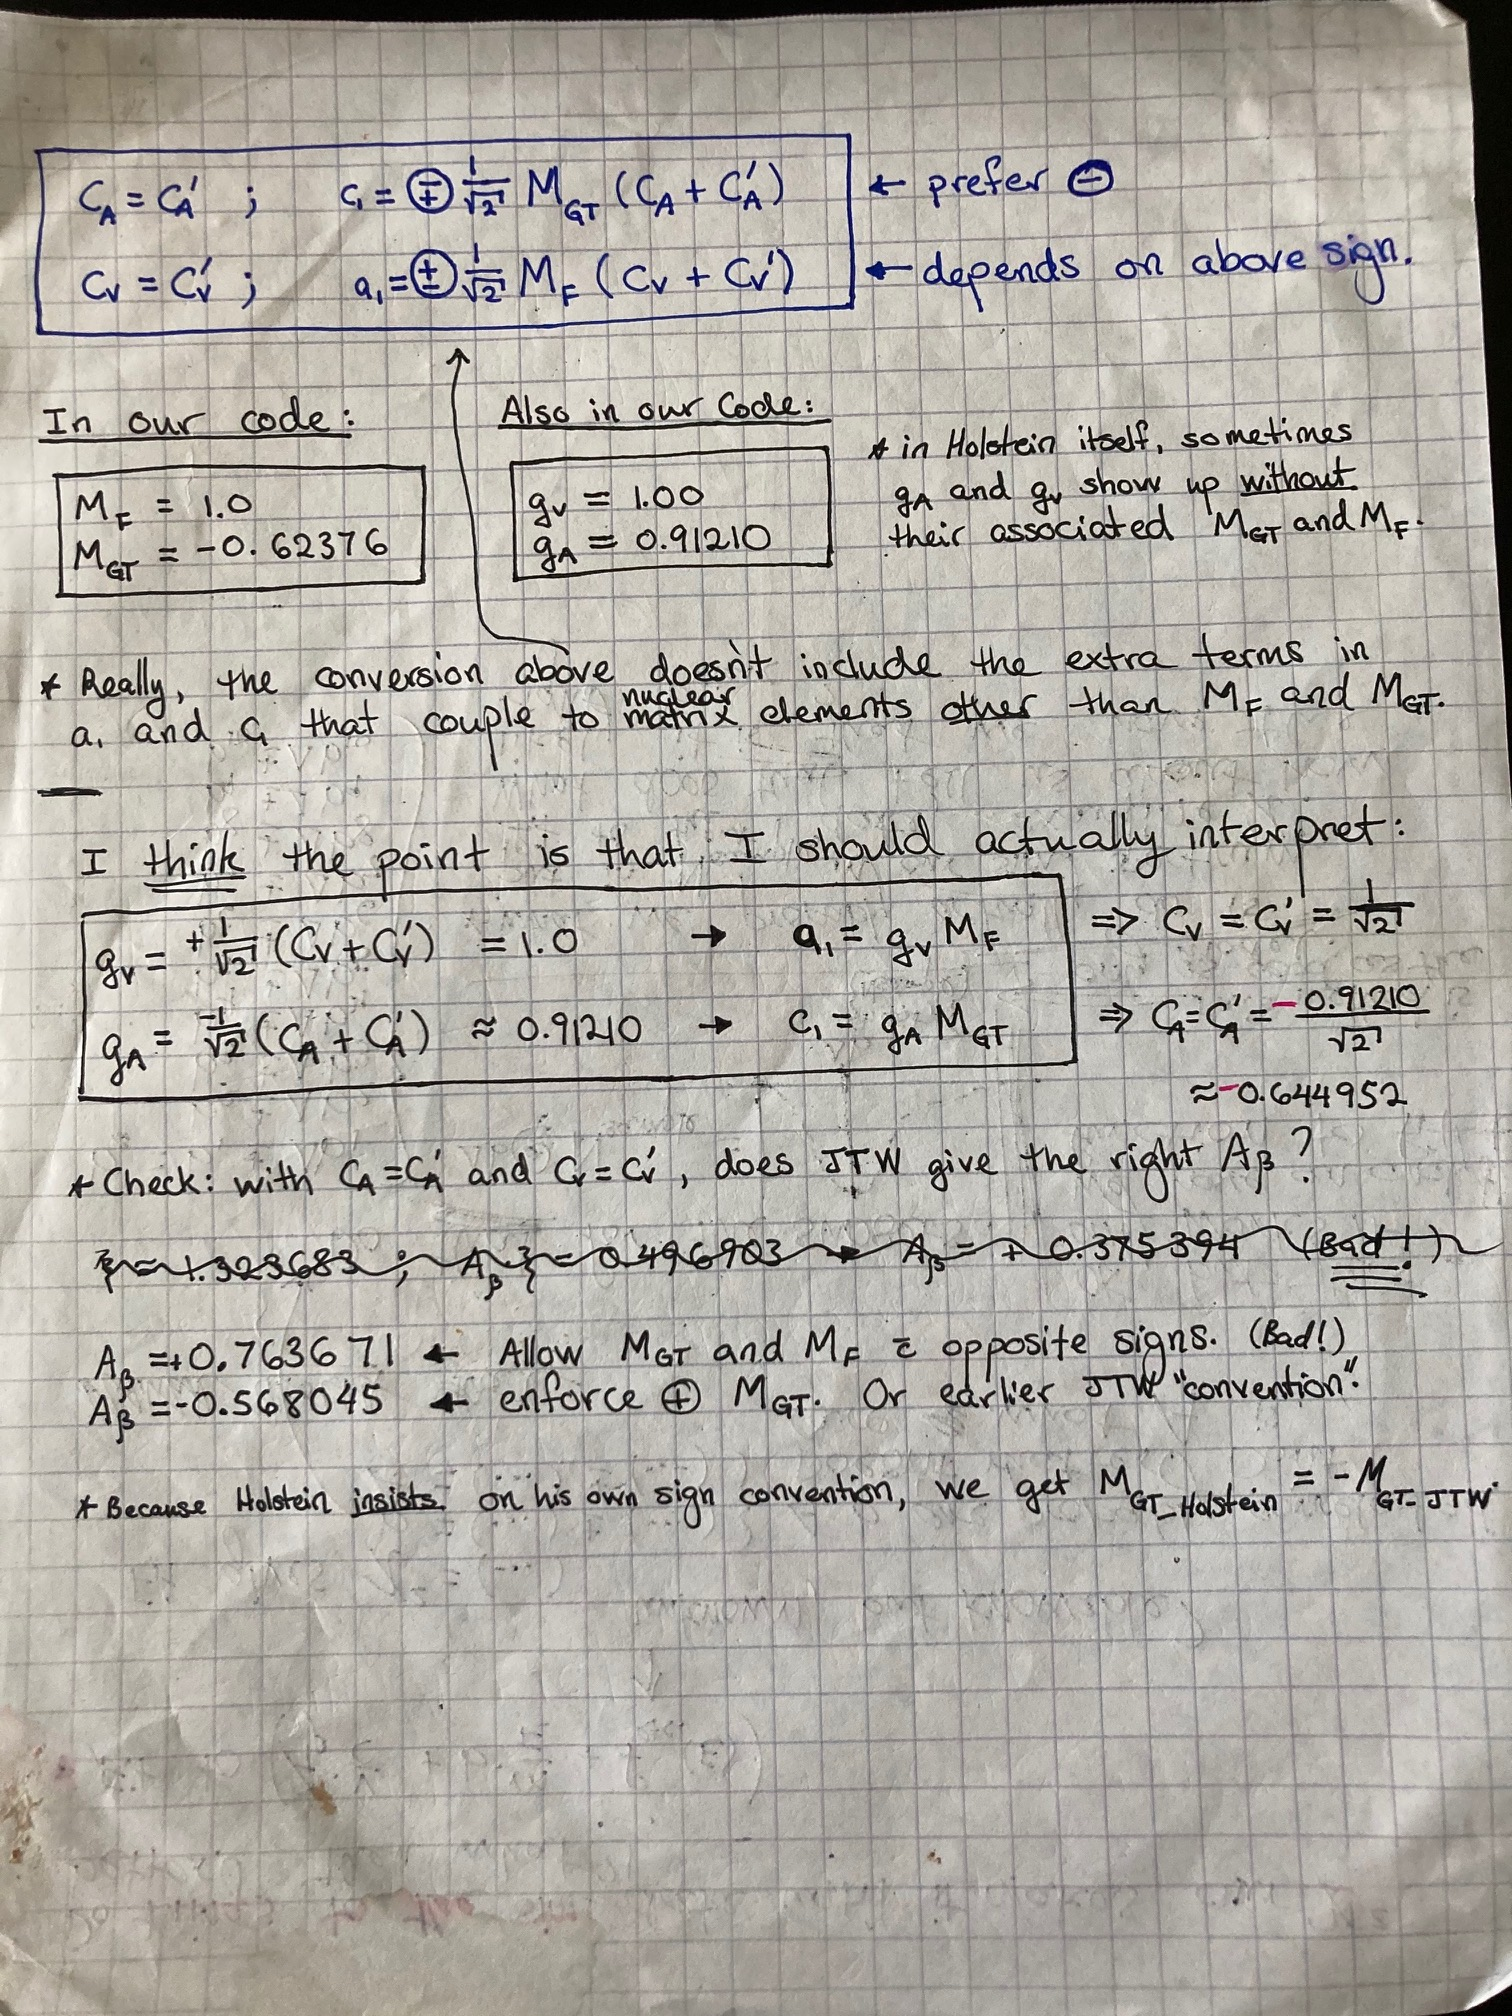
\includegraphics[width=.999\linewidth]
	{Figures/oldnotes_holstein_jtw/image0.jpg} }
	\caption{"Notes 0"}
	\label{fig:notes0}
\end{figure}

\begin{figure}[htb]
	\centering
	{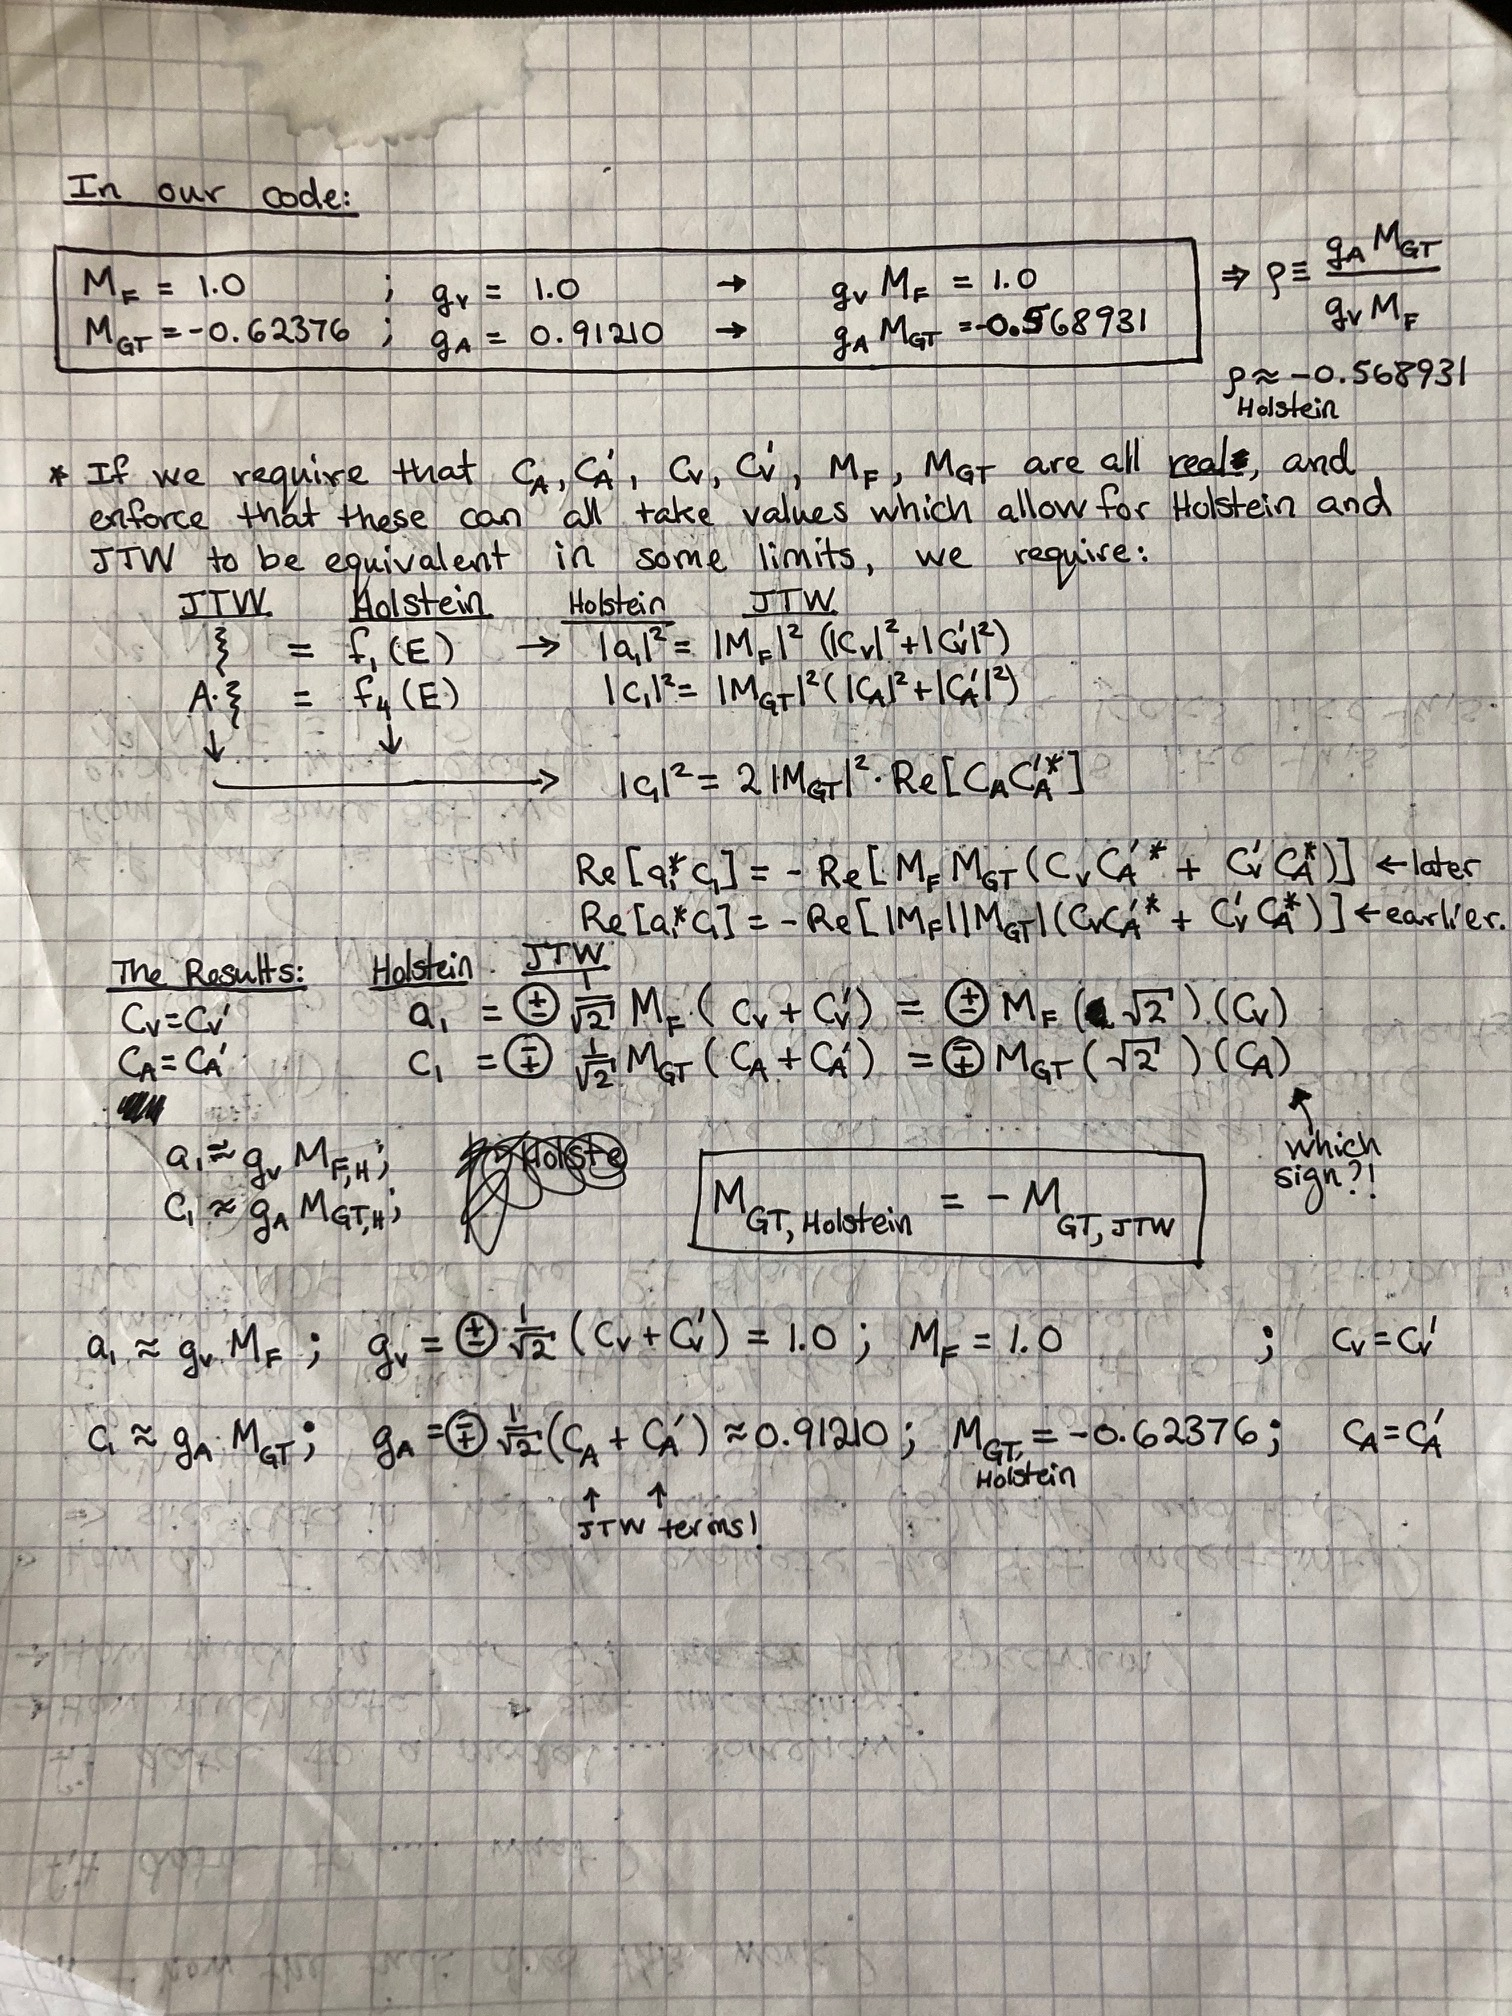
\includegraphics[width=.999\linewidth]
	{Figures/oldnotes_holstein_jtw/image1.jpg} }
	\caption{"Notes 1"}
	\label{fig:notes1}
\end{figure}

\begin{figure}[htb]
	\centering
	{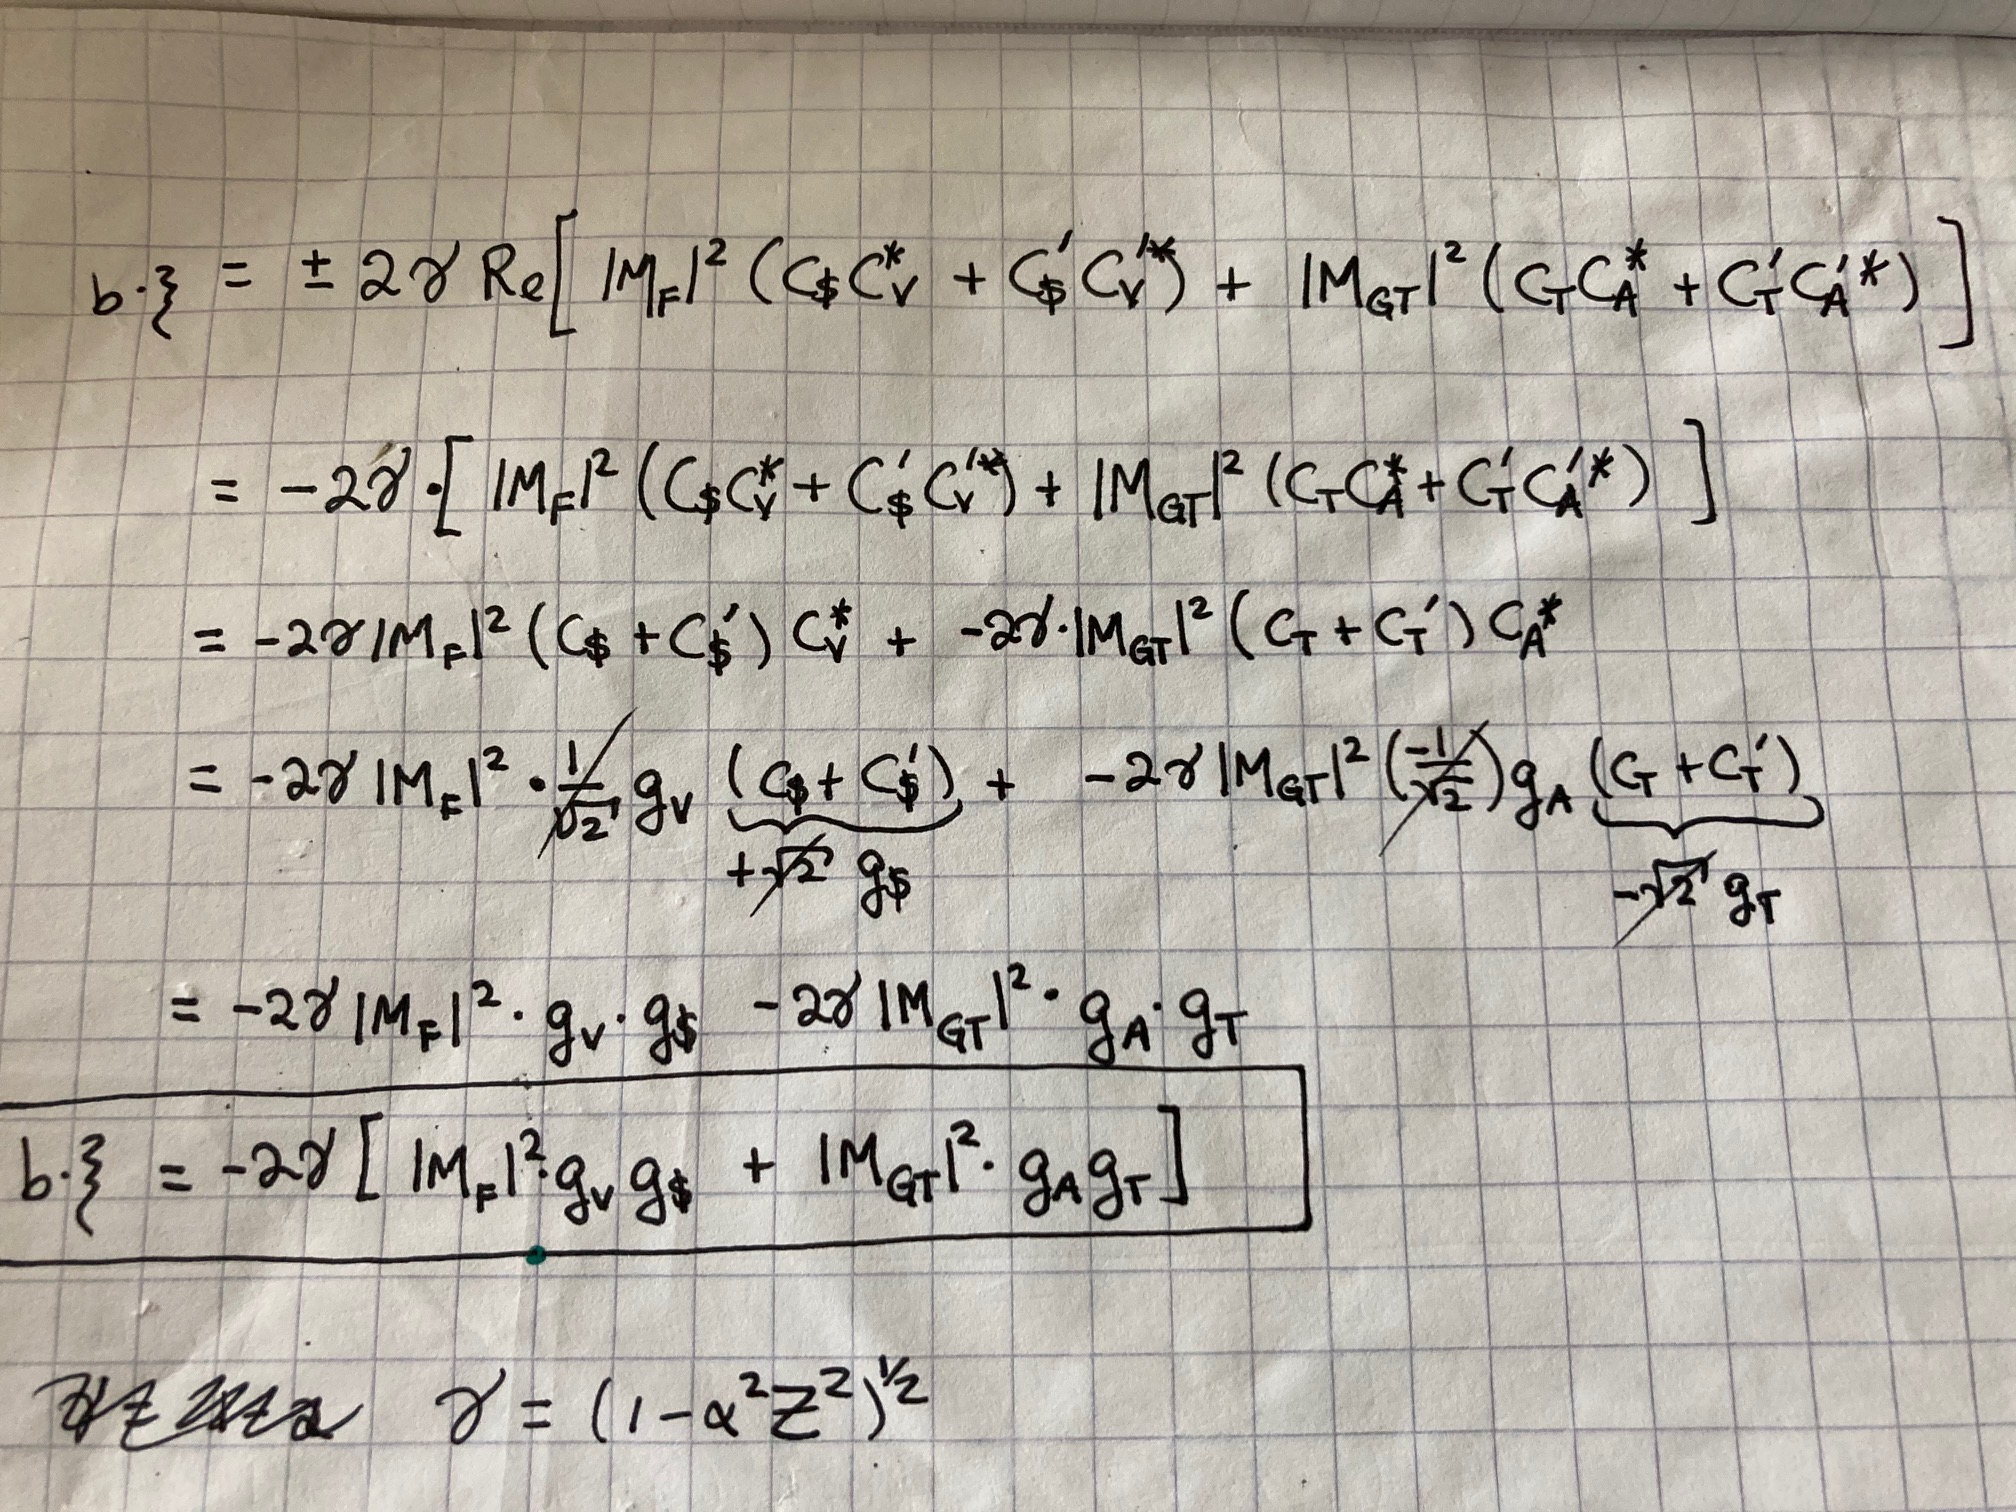
\includegraphics[width=.999\linewidth]
	{Figures/oldnotes_holstein_jtw/image2.jpg} }
	\caption{"Notes 2"}
	\label{fig:notes2}
\end{figure}

\begin{figure}[htb]
	\centering
	{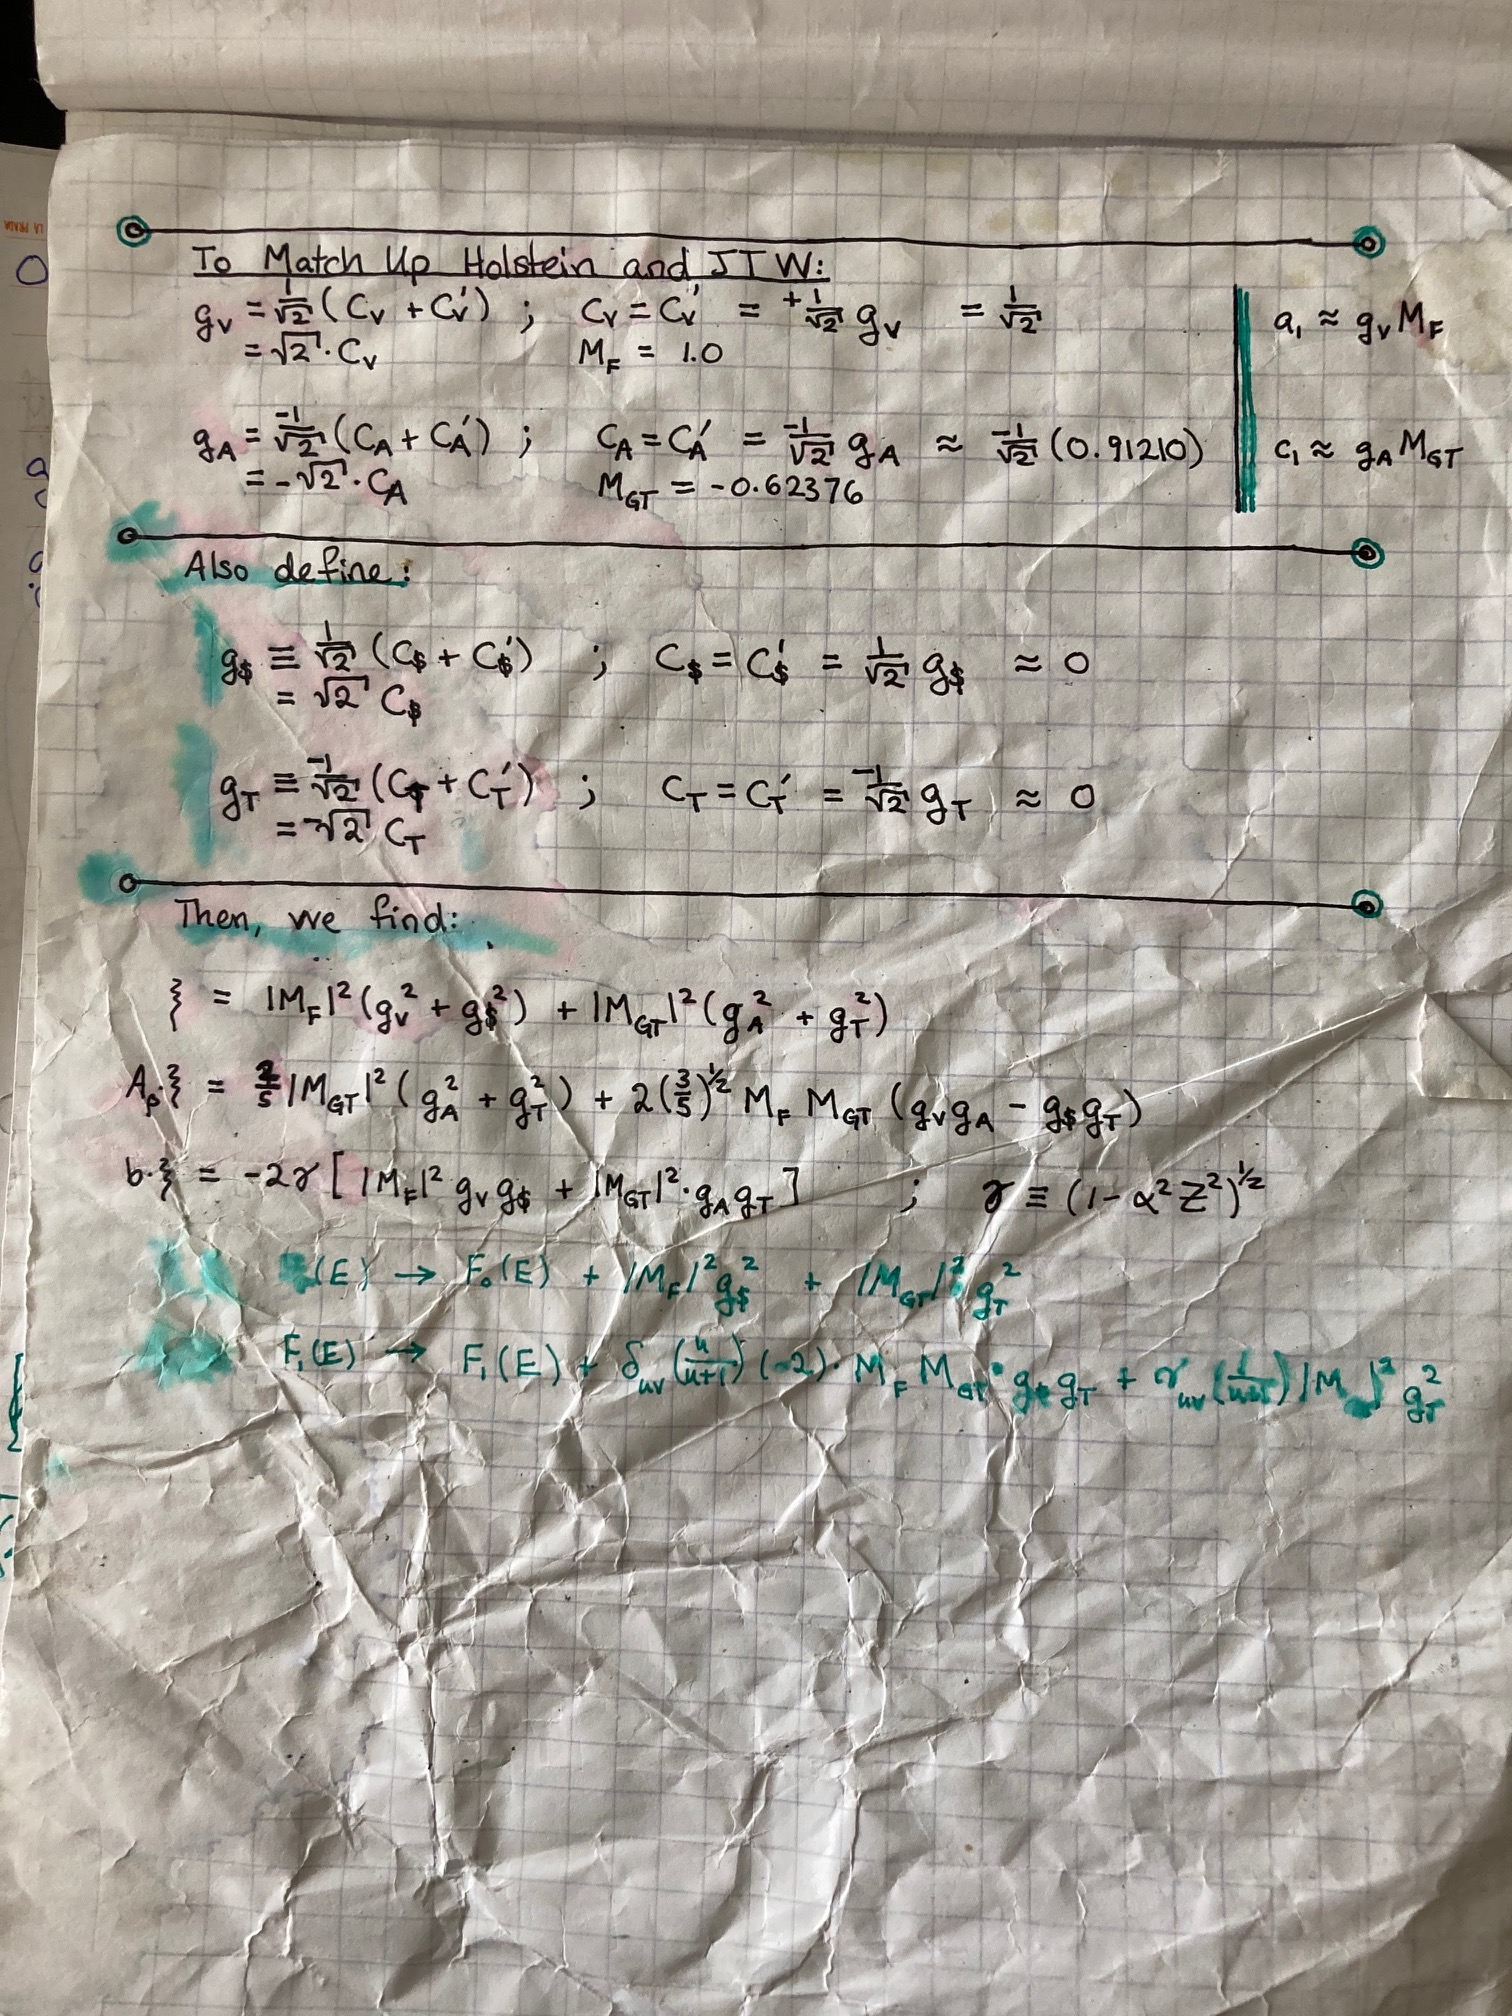
\includegraphics[width=.999\linewidth]
	{Figures/oldnotes_holstein_jtw/image3.jpg} }
	\caption{"Notes 3"}
	\label{fig:notes3}
\end{figure}

\begin{figure}[htb]
	\centering
	{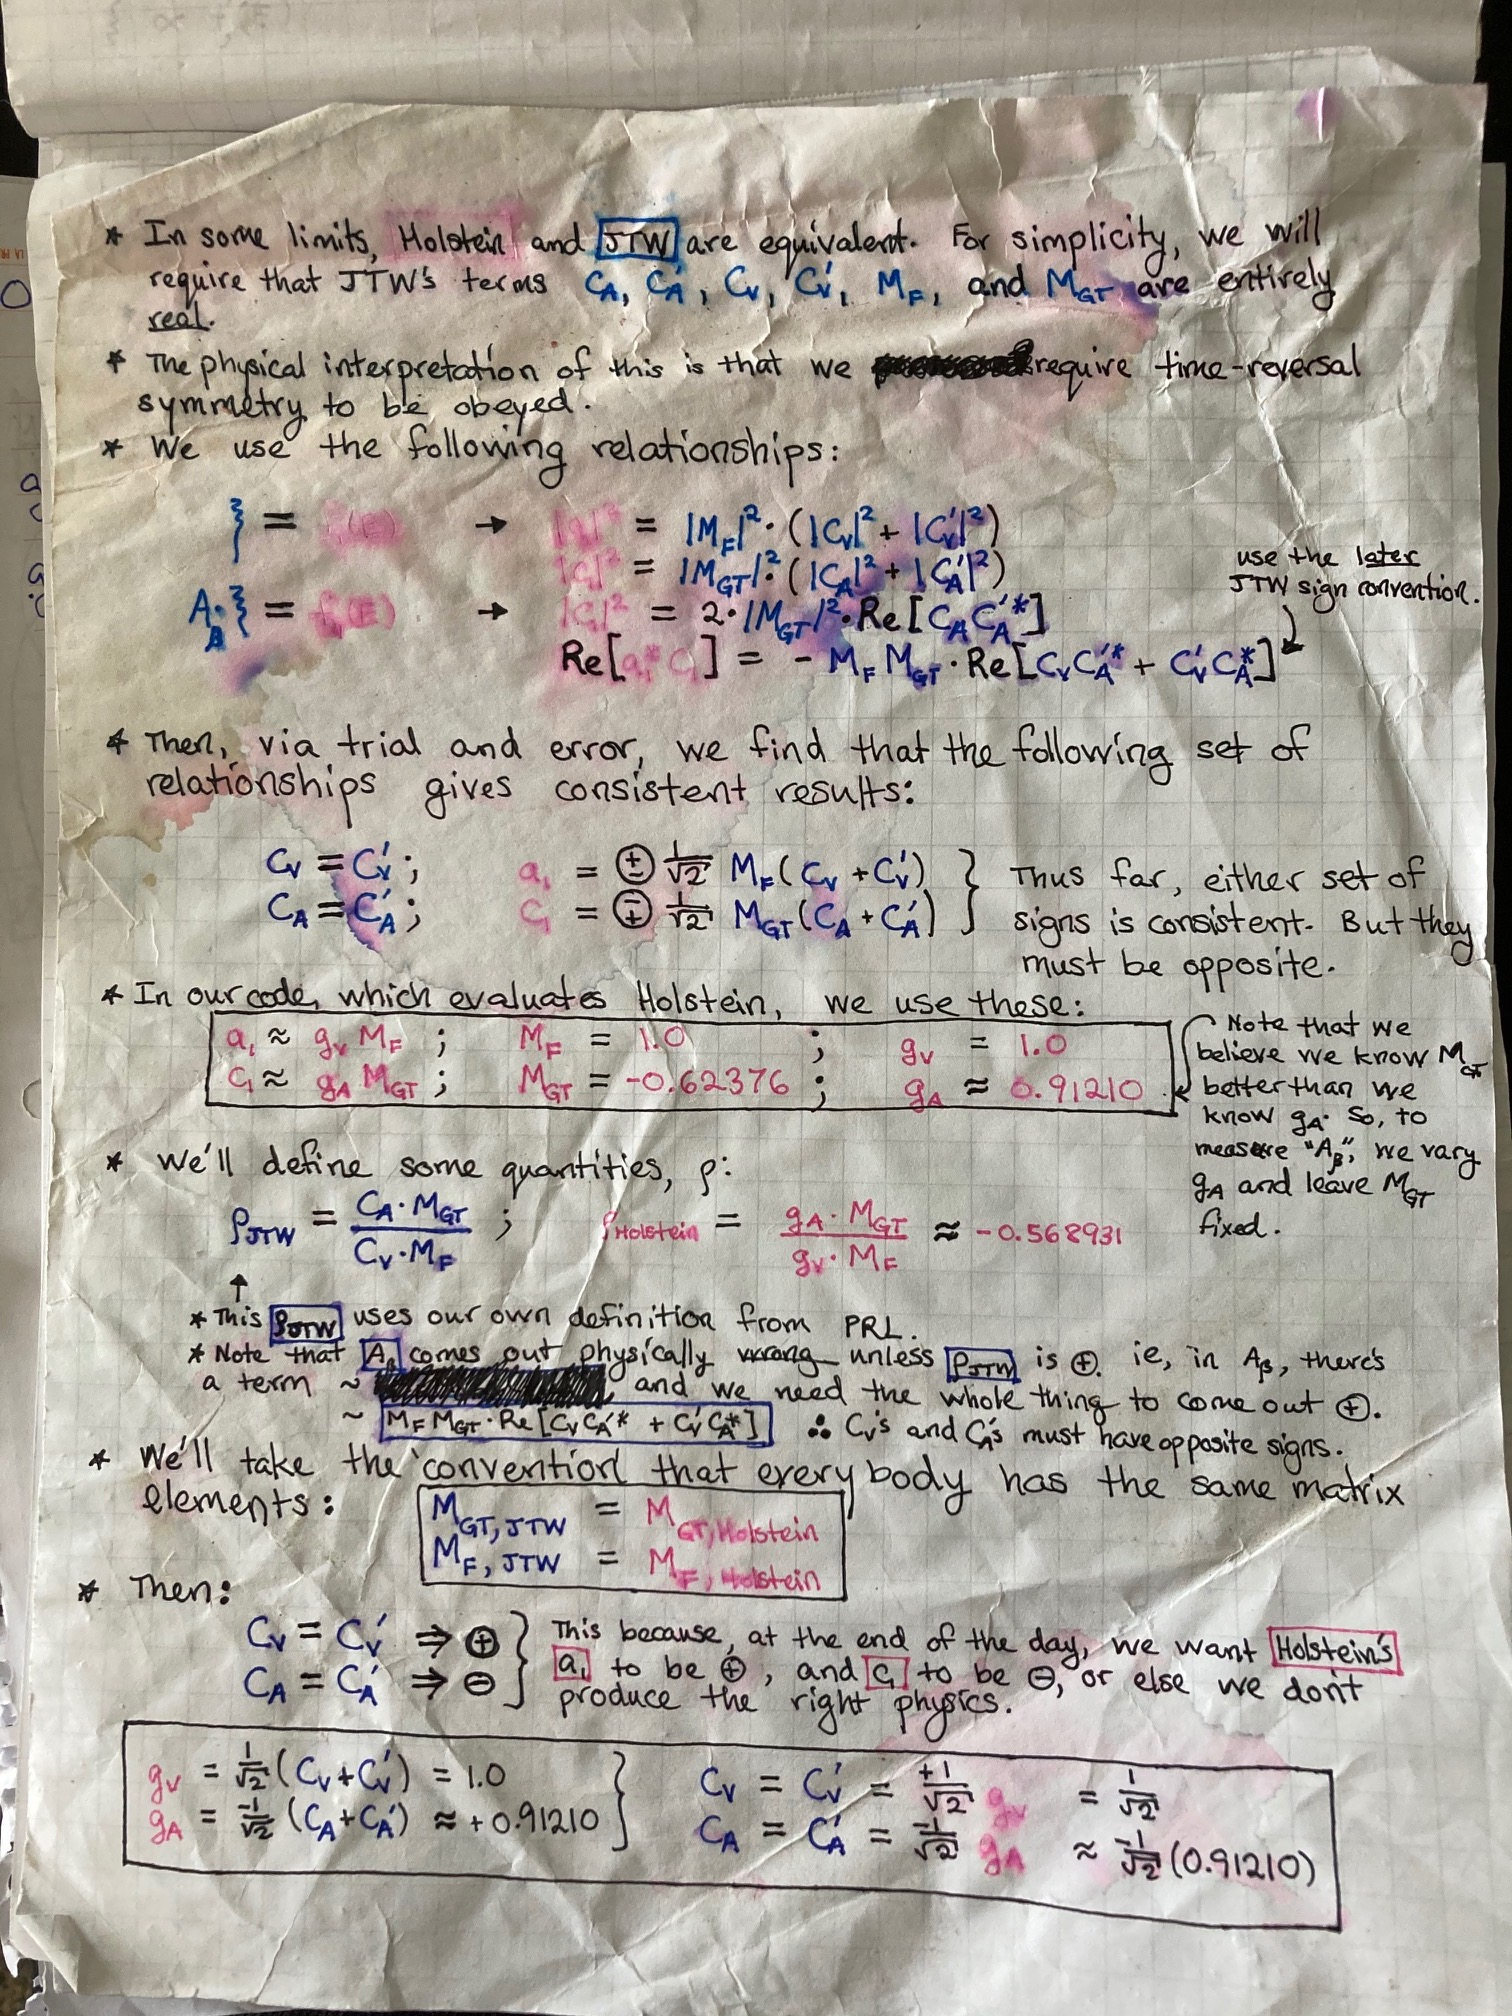
\includegraphics[width=.999\linewidth]
	{Figures/oldnotes_holstein_jtw/image4.jpg} }
	\caption{"Notes 4"}
	\label{fig:notes4}
\end{figure}

\begin{figure}[htb]
	\centering
	{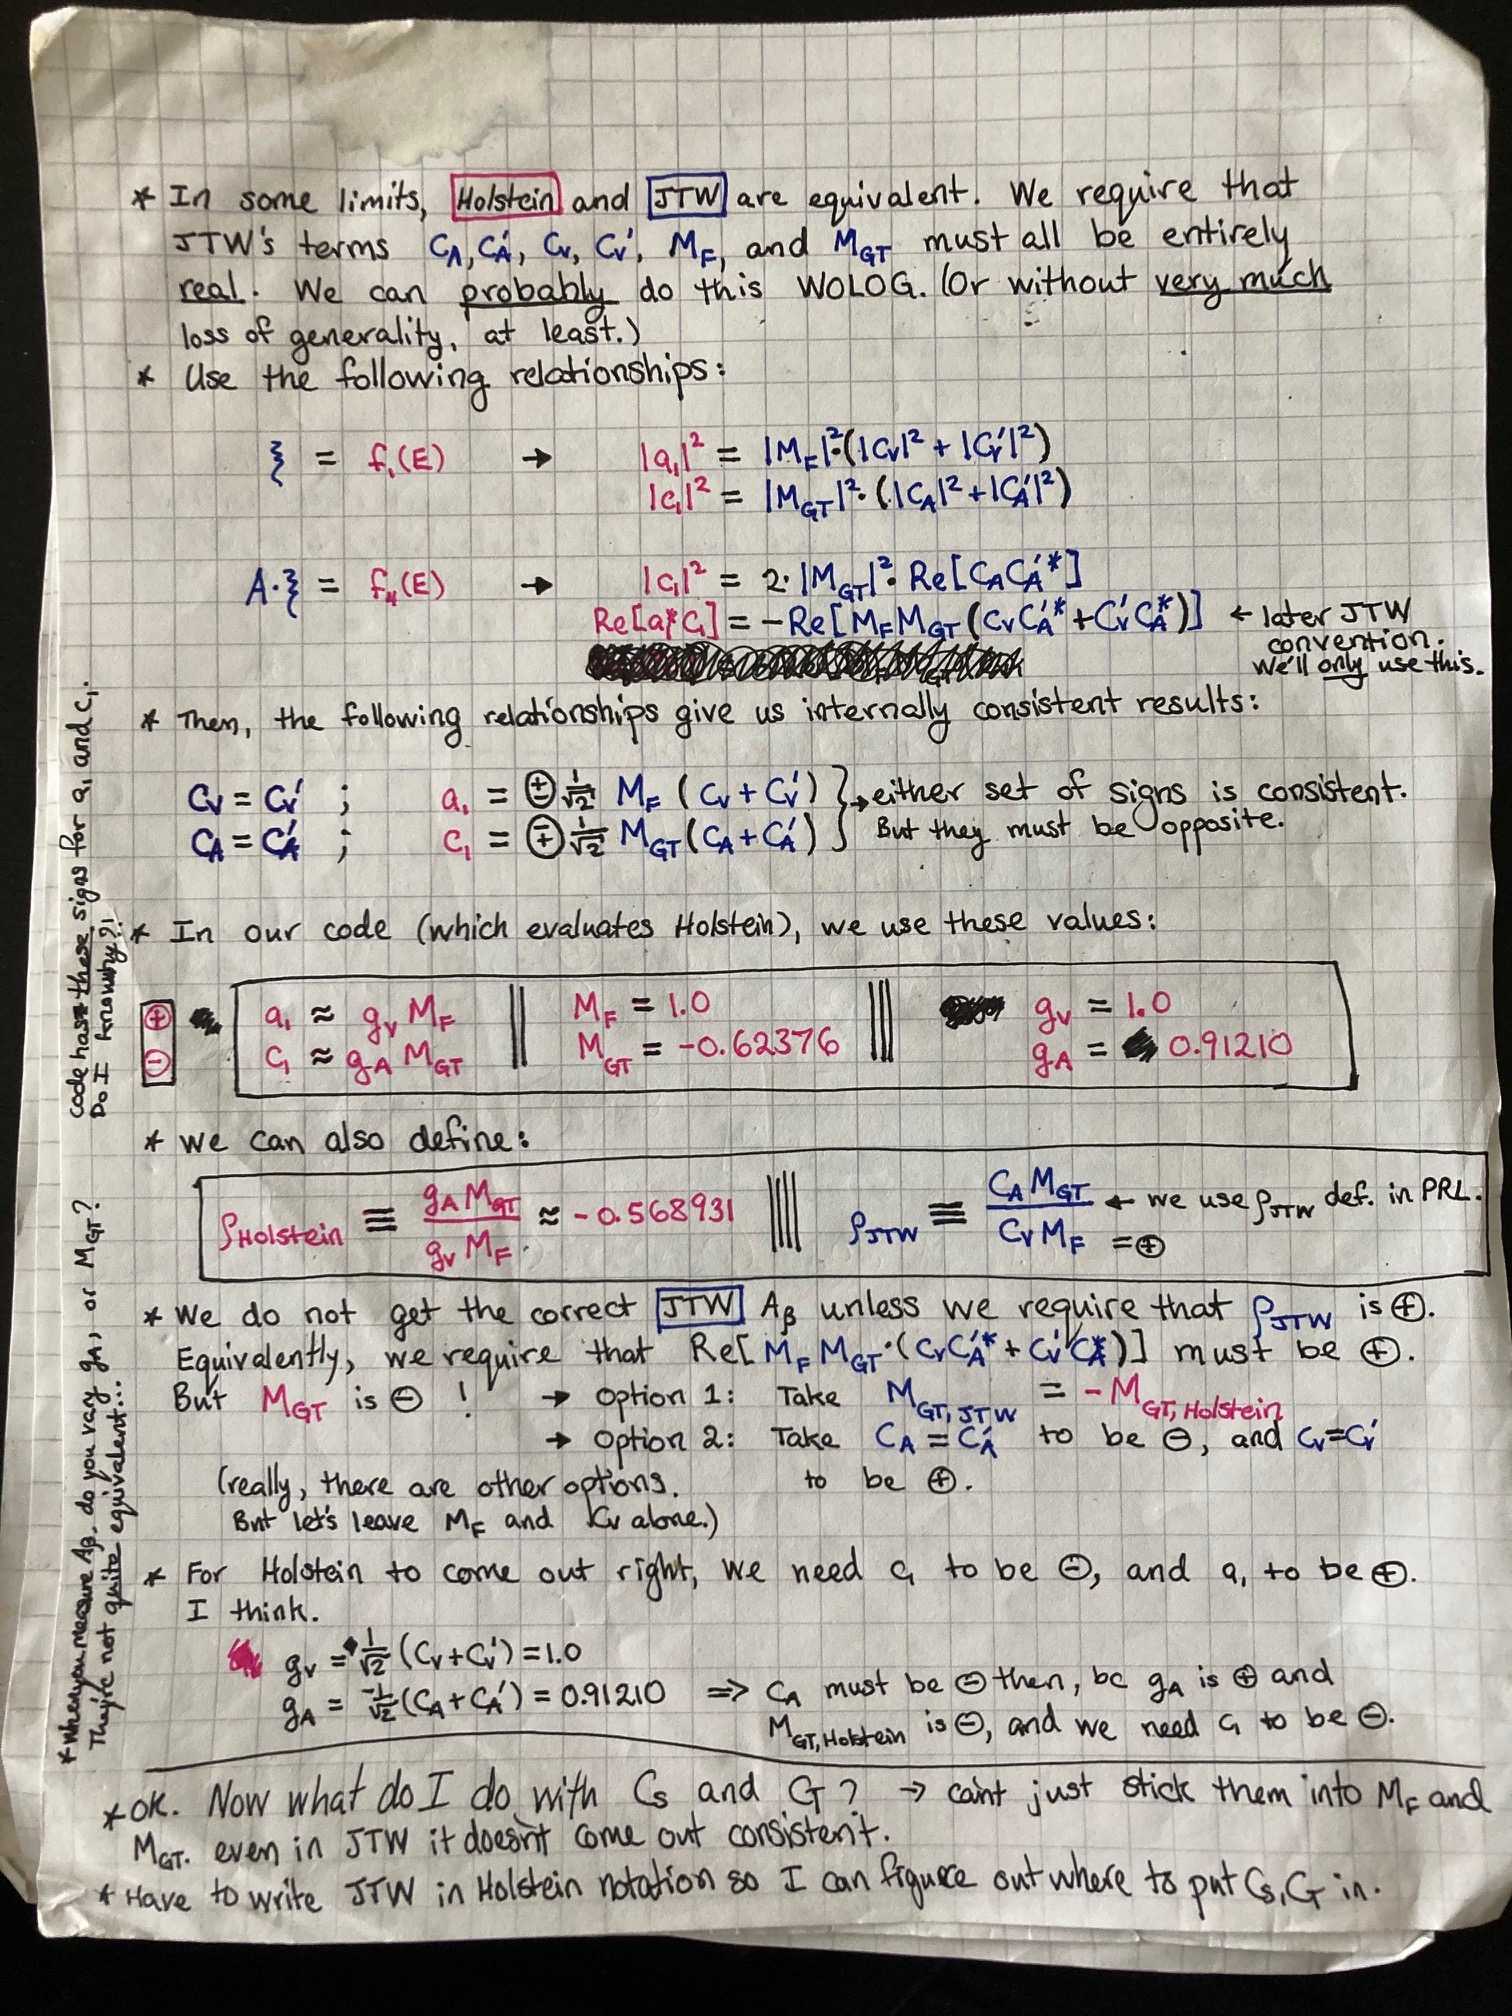
\includegraphics[width=.999\linewidth]
	{Figures/oldnotes_holstein_jtw/image5.jpg} }
	\caption{"Notes 5"}
	\label{fig:notes5}
\end{figure}
     % JB says:  Keep App. C after some tweaks.
% !TEX root = ../thesis_main.tex



%%%% --- * --- %%%%	
\chapter[Holstein/JTW Comparison Confusion]{Holstein/JTW Comparison Confusion}

\note[color=jb]{Appendix D (that's this!) -> internal document.}
\note{I see a couple things here that I want to keep.  That stuff probably gets moved to Appendix C. }
\note[color=jb]{JB:  Appendix C has some redundancies with B. You will have to sort that out.
The page-long shaggy dog story of f7 is distracting and needs to be truncated
to the insight gained: "f7 is a recoil order term, and there are no recoil order
terms in JTW." There may be many nore things to do of that sort.  
\\
...
\\
MJA:  There's fuck all mention of f7 in Appendix C at the time of this comment, so he probably meant Appendix D.  Probably there are redundancies everywhere though.}


Ben at pg 17(30) claims the relation between JTW and Holstein for $\Abeta$ is:

\begin{equation}
\Abeta = \frac{f_4(E)+ \frac{1}{3}f_7(E)}{f_1(E)}
\end{equation}

See, it's counterintuitive, because I would have guessed that it would be just

\begin{equation}
A_\beta = \frac{f_4(E)}{f_1(E)}
\end{equation}

...But it's not.  That extra $f_7$ term is there, being weird.  In Holstein (51), it's all like, 
\begin{equation}
d^5\Gamma = (...) + (...)*\Lambda_1 (\hat{n} \cdot \hat{k}) (\frac{\vec{p}}{E}\cdot \hat{k} )\,f_7(E), 
\end{equation}

and that just doesn't look like $\Abeta$.

So, maybe there's some magic that happens when you integrate it and it turns into (52). 
From (52), I would (naively??) think that:

\begin{equation}
A_\beta = \frac{F_1(E)}{F_0(E)}
\end{equation}

Is it even true?!?  Let's see what Holstein has to say...

In general, 
\begin{eqnarray}
f_i(E) &=& F_i(E, J, J^\prime, 0) \\
F_i(E) &=& H_i(E, J, J^\prime, 0)
\end{eqnarray}

So here specifically, we have: 
\bea
	F_0(E) = H_0(E, u, v, s) &=& F_1(E, u, v, s) \\ 
	F_1(E) = H_1(E, u, v, s) &=& F_4(E, u, v, s) + \frac{1}{3}F_7(E, u, v, s) \\
                             &=& f_4(E) + \frac{1}{3}f_7(E)
\eea

So I guess whatever the fuck Ben did to get his result checks out, and my naive supposition was correct.  But now how do I translate that into JTW for anything else?!  

JTW just straight-up has *nothing* that corresponds to the $f_7$ term in Holstein.  The integral that puts $f_7$ into $A_\beta$ has simply *not been done* at the point where JTW writes down their equation.

So, okay, let's take a look at how the dominant terms in $f_4$, $f_1$, and $f_7$ scale.  From Holstein (pg 807):
\bea
	f_1(E) & \approx & a_1^2 + c_1^2 \\
	f_4(E) & \approx & \mathrm{(const)}*2 a_1 c_1 +\mathrm{(const)}c_1^2 \\
	f_7(E) & \approx & \mathrm{(const)}*a_1 c_1 \frac{E0}{M} +\mathrm{(const)}a_1 c_1 \frac{E}{M} + \mathrm{(const)}c_1^2 \frac{E0}{2M} + \mathrm{(const)}c_1^2 \frac{E}{2M}
\eea

OK, so I think $f_7$ wouldn't be included in JTW anyway, because it's too high order in $E/M$.  (Is there really nothing in $f_7$ that's not multiplied by at least one factor of $1/M$ ?? .... yep, nothing.)

So here's what Coulomb-JTW says (set $C_S=C_S^\prime=C_T=C_T^\prime=0$, and require that $C_A=C_A^\prime$ and $C_V=C_V^\prime$ are real):

\begin{eqnarray}
\xi         &=& |M_F|^2( 2 C_V^2) + |M_{GT}|^2(2 C_A^2) \\
A_\beta \xi &=& |M_{GT}|^2 \frac{1}{J+1} \left[ +2 C_A^2 + M_F M_{GT} \left(\frac{J}{J+1}\right)^{1/2} *(-2 C_V C_A) \right]
\end{eqnarray}

Indeed, there are no E/M terms.  So we agree with ourselves here.  That's nice.  
But actually, we need to figure out how to convert *all* of the JTW letters into Holstein notation.  Not just $\Abeta$.  Of particular importance is anything with a *linear* dependence on $C_T$ (or $C_S$).  That includes $bFierz$, for which there is no Holstein equivalent, but also:

\begin{itemize}
	\item Real parts of $\bFierz$
	\item Imaginary parts of $\abetanu$
	\item Imaginary parts of $\calign$
	\item Imaginary parts of $\Abeta$
	\item Real parts of $\Bnu$
	\item Real parts of $\DTR$
\end{itemize}

...which is actually all of the things.  All of them.  So, I claim these are the relationships:

\begin{eqnarray}
\xi          &=& f_1(E) \;\;\;\;\;\; \;\;\;\;\;\; \;\;\;\; (?) \\
a_{\beta\nu} &=& f_2(E) \: / \: f_1(E) \\
\frac{\langle\vec{J}\rangle}{J} \cdot \frac{\vec{p}}{E} \,\, A_\beta 
  &=& \Lambda_1 \hat{n}\cdot \frac{\vec{p}}{E} \, f_4(E) \:/\: f_1(E) \\
\frac{\langle\vec{J}\rangle}{J} \cdot \frac{\vec{p}_\nu}{E_\nu} B_\nu  
  &=& \Lambda_1 \hat{n} \cdot \vec{k} \;\;\, f_6(E) \:/\: f_1(E) \\
\frac{\langle\vec{J}\rangle}{J} \cdot \frac{\left( \vec{p} \times \vec{p}_\nu \right)}{E_{} E_\nu} D_{\mathrm{TR}} 
  &=& \Lambda_1 \hat{n} \cdot ( \frac{\vec{p}}{E} \times \hat{k} \,) \;\; f_8(E) \:/\: f_1(E) \\
\left[ \frac{J(J+1) - 3\langle (\vec{J}\cdot\hat{j})^2 \rangle}{J(2J-1)} \right] \!\!\!
\left[\frac{1}{3} \frac{\vec{p}\cdot\vec{p}_\nu }{E_{} E_\nu} - \frac{ (\vec{p}\cdot\hat{j}) (\vec{p}_\nu \cdot\hat{j} ) }{E_{} E_\nu} \right]c_{\mathrm{align}} 
  &=& \Lambda_2 \! \left[(\hat{n}\cdot\frac{\vec{p}}{E})(\hat{n}\cdot\hat{k})  - \frac{1}{3} (\frac{\vec{p}}{E}\cdot\hat{k} \,)\right] \; f_{12}(E) \:/\: f_1(E)
\end{eqnarray}

Other Holstein terms in (51) have no JTW equivalent, either because JTW didn't include recoil-order corrections, or because JTW didn't bother with higher multipole moments.  These Holstein-specific spectral functions are not used in JTW:

\begin{itemize}
	\item $f_{3}(E)$  (dipole)
	\item $f_{5}(E)$  (dipole)
	\item $f_{7}(E)$  (dipole)
	\item $f_{9}(E)$  (dipole)
	\item $f_{10}(E)$ (quadrupole)
	\item $f_{11}(E)$ (quadrupole)
	\item $f_{13}(E)$ (quadrupole)
	\item $f_{1}(E)$  (quadrupole, used elsewhere)
	\item $f_{16}(E)$ (quadrupole)
	\item $f_{17}(E)$ (quadrupole)
	\item Octopoles:  $f_{18}$, $f_{19}$, $f_{20}$, $f_{21}$, $f_{22}$, $f_{23}$, $f_{24}$
	\item 16-poles:   $f_{25}$, $f_{26}$, $f_{27}$.
\end{itemize}

OK, so what needs to happen now is for me to convert the JTW alphabet into *other* Holstein notation.  Since I know how they scale with the $f_i(E)$'s, let's see if we can convert those specific $f_i(E)$'s into any of the Holstein notation that is going into my code -- ie, the $F_i(E)$'s.  In particular, we'll want $f_1(E)$, $f_2(E)$, $f_4(E)$, $f_6(E)$, $f_8(E)$, $f_12(E)$.  This will actually have the pleasant side-effect of telling us how to fucking do that goddamn neutrino momentum integral in JTW.  I think.  So, from Holstein:

\begin{itemize}
	\item $f_1(E) \; = \; F_1\;(E, u, v, s) \; = \; H_0(E, u, v, s) = F_0(E) $
	\item $f_2(E) \; = \; F_2\;(E, u, v, s) \; = \; ? $
	\item $f_4(E) \; = \; F_4\;(E, u, v, s) \; = \; ? $
	\item $f_6(E) \; = \; F_6\;(E, u, v, s) \; = \; ? $
	\item $f_8(E) \; = \; F_8\;(E, u, v, s) \; = \; ? $
	\item $f_{12}(E) = \; F_{12}(E, u, v, s)\; = \; ? $
\end{itemize}

...which, let's be honest, doesn't really help.  Let's go the other direction, then.

\begin{itemize}
	\item $ F_0(E) = H_0(E, u, v, s) = F_1(E, u, v, s)    = f_1(E) $    as before, but also:
	\item $ F_1(E) = H_1(E, u, v, s) = F_4(E, u, v, s) + \frac{1}{3} F_7(E, u, v, s)  = f_4(E) + \frac{1}{3} f_7(E) $
	\item $ F_2(E) = H_2(E, u, v, s) = F_{10}(E, u, v, s) + \frac{1}{3} F_{13}(E, u, v, s) = f_{10}(E) + \frac{1}{3} f_{13}(E) $ 
	\item $ F_3(E) = H_3(E, u, v, s) = F_{18}(E, u, v, s) = f_{18}(E)$ 
\end{itemize}

So, okay, I can write *my* PDF in terms of only Holstein's $ f_1(E)$,  $f_4(E)$,  $f_7(E)$,  $f_{10}(E)$,  $f_{13}(E)$,  $f_{18}(E)$.  I can write JTW's PDF in terms of only Holstein's $f_1(E)$,  $f_2(E)$,  $f_4(E)$,  $f_6(E)$,  $f_8(E)$,  $f_{12}(E)$.  Those ... aren't the same thing.  Like, at all.  If I integrate those, do they come out to be the same things?  Somehow?  

OK.  I can separate some terms out into what they *should* correspond to based on their multipole dependence...  Roughly speaking, 

\begin{eqnarray}
F_0(E) &\leftrightarrow& f_1(E) \;\;\; \mathrm{    (obviously)} \\
F_1(E) &\leftrightarrow& f_4(E), \; f_5(E), \; f_6(E), \; f_7(E), \; f_8(E), \; f_9(E) \\
F_2(E) &\leftrightarrow& f_{10}(E), \; f_{11}(E), \; f_{12}(E), \; f_{13}(E), \; f_1(E), \; f_{16}(E) \\ 
F_3(E) &\leftrightarrow& \; \textrm{...who even cares?}
\end{eqnarray}


\begin{itemize}
	\item * Check: in Holstein, are there simple relationships between those things?  
	\item * Check: if I do the integrals of the momentum-thingies multiplying those specific $f_i(E)$'s in Eq. (51) do they turn out the way I expect?  ie, do I recover the corresponding terms in Eq. (52)? 
\end{itemize}

 % JB says:  Appendix D -> internal document
\chapter[Multipole Comparisons]{Compare by Multipoles!}

My code uses Holstein's Eq. (52), rather than Eq. (51).  In his notation, I'm using $F_i(E)$'s rather than $f_i(E)$'s.  I need to convert between them.  
This is because:
\begin{itemize}
	\item
(a):  Coulomb/Radiative corrections ( some terms, up to $f_15(E)$ ):  \\
		$f_1$, $f_2$, $f_4$, $f_6$, $f_7$, $f_12$, $f_14$, $f_15$    
	\item
(b):  $C_S$/$C_T$ inclusion (JTW has equivalents for only some terms, up to $f_12(E)$): \\
		$f_1$, $f_2$, $f_4$, $f_6$, $f_8$, $f_12$.
\end{itemize}

Holstein and JTW terms have *this* relationship:
\begin{eqnarray}
\xi          &=& f_1(E) \;\;\;\;\;\; \;\;\;\;\;\; \;\;\;\;\;\; \textrm{(? times some constant?  doesn't matter.)} \\
a_{\beta\nu} &=& f_2(E) \: / \: f_1(E) \\
\frac{\langle\vec{J}\rangle}{J} \cdot \frac{\vec{p}}{E} \,\, A_\beta 
  &=& \Lambda_1 \hat{n}\cdot \frac{\vec{p}}{E} \, f_4(E) \:/\: f_1(E) \\
\frac{\langle\vec{J}\rangle}{J} \cdot \frac{\vec{p}_\nu}{E_\nu} B_\nu  
  &=& \Lambda_1 \hat{n} \cdot \vec{k} \;\;\, f_6(E) \:/\: f_1(E) \\
\frac{\langle\vec{J}\rangle}{J} \cdot \frac{\left( \vec{p} \times \vec{p}_\nu \right)}{E_{} E_\nu} D_{\mathrm{TR}} 
  &=& \Lambda_1 \hat{n} \cdot ( \frac{\vec{p}}{E} \times \hat{k} \,) \;\; f_8(E) \:/\: f_1(E) \\
\left[ \frac{J(J+1) - 3\langle (\vec{J}\cdot\hat{j})^2 \rangle}{J(2J-1)} \right] \!\!\!
\left[\frac{1}{3} \frac{\vec{p}\cdot\vec{p}_\nu }{E_{} E_\nu} - \frac{ (\vec{p}\cdot\hat{j}) (\vec{p}_\nu \cdot\hat{j} ) }{E_{} E_\nu} \right]c_{\mathrm{align}} 
  &=& \Lambda_2 \! \left[(\hat{n}\cdot\frac{\vec{p}}{E})(\hat{n}\cdot\hat{k})  - \frac{1}{3} (\frac{\vec{p}}{E}\cdot\hat{k} \,)\right] \; f_{12}(E) \:/\: f_1(E)
\end{eqnarray}


\begin{itemize}
	\item
JTW Monopole Terms:
$\xi,  \;\;\;\;\;
\xi \frac{m}{E}*b_{\textrm{Fierz}},  \;\;\;\;\;
\xi \frac{\vec{p} \cdot \vec{p}_\nu}{E_{} E_\nu} * a_{\beta\nu} $

	\item
JTW Dipole Terms:
$\xi \frac{\langle \vec{J} \rangle}{J} \cdot \frac{\vec{p}}{E} * A_\beta, \;\;\;\;\;
\xi \frac{\langle \vec{J} \rangle}{J} \cdot \frac{\vec{p}_\nu}{E_\nu} * B_\nu,  \;\;\;\;\;
\xi \frac{\langle \vec{J} \rangle}{J} \cdot \frac{\vec{p} \times \vec{p}_\nu }{E_{} E_\nu} * D_{\mathrm{TR}}$ 

	\item
JTW Quadrupole Terms:
$\xi \left(\!\! \frac{J(J+1) - 3\langle (\vec{J} \cdot \hat{j})^2 \rangle }{J(2J-1)} \!\!\right) \!\!
\left(\!\! \frac{1}{3}\frac{\vec{p}\cdot\vec{p}_\nu}{E_{} E_\nu} - \frac{(\vec{p}\cdot\hat{j})(\vec{p}_\nu \cdot \hat{j})}{E_{} E_\nu} \!\!\right) * c_{\textrm{align}}
$
\end{itemize}

...

\begin{itemize}
	\item
Holstein (52) Monopole Term: \\
$F_0(E) = f_1(E)$
	
	\item
Holstein (52) Dipole Term: \\
$\Lambda_1 \,( \hat{n} \cdot \frac{\vec{p}}{E} )\,* \, F_1(E) \\
\;\;\;\;\; = \Lambda_1 \,( \hat{n} \cdot \frac{\vec{p}}{E} ) * \! \left(\, f_4(E) + \frac{1}{3}f_7(E) \right) $
	
	\item
Holstein (52) Quadrupole Term: \\
$\Lambda_2 \left( (\hat{n}\cdot \frac{\vec{p}}{E})^2 - \frac{1}{3} \frac{p^2}{E^2} \right) * F_2(E) \\ 
\;\;\;\;\; = \Lambda_2 \left( (\hat{n}\cdot \frac{\vec{p}}{E})^2 - \frac{1}{3} \frac{p^2}{E^2} \right)  *\! \left(\, f_{10}(E) + \frac{1}{3} f_{13}(E) \right) \\
\;\;\;\;\; = \Lambda_2 T_2(\hat{n}):[\frac{\vec{p}}{E}, \frac{\vec{p}}{E}] 
  *\! \left(\, f_{10}(E) + \frac{1}{3} f_{13}(E) \right)
$

	\item
Holstein (52) Octopole Term: \\
$\Lambda_3 
\left( (\hat{n} \cdot \frac{\vec{p}}{E} )^3 - \frac{3}{5} \frac{p^2}{E^2} (\hat{n}\cdot \frac{\vec{p}}{E}) \right) 
* F_3(E) \\
\;\;\;\;\; = \Lambda_3
\left( (\hat{n} \cdot \frac{\vec{p}}{E} )^3 - \frac{3}{5} \frac{p^2}{E^2} (\hat{n}\cdot \frac{\vec{p}}{E}) \right) 
* \, f_{18}(E) \\
\;\;\;\;\; = \Lambda_3 T_3(\hat{n}):[\frac{\vec{p}}{E}, \frac{\vec{p}}{E}, \frac{\vec{p}}{E} ] 
* \, f_{18}(E)
$
	\item
Holstein (52) Hexadecapole Term: \\
$\textrm{(none)}$
\end{itemize}

...

\begin{itemize}

	\item
Holstein (51) Monopole Terms: \\ 
$f_1(E),  \;\;\;\;\; 
\frac{\vec{p}\cdot \hat{k} }{E}* f_2(E), \;\;\;\;\; 
\left(\! \frac{ (\vec{p}\cdot\hat{k})^2 }{E^2}  - \frac{1}{3}\frac{p^2}{E^2} \!\right)\! * f_3(E)$

	\item
Holstein (51) Dipole Terms: \\
$\Lambda_1 \,( \hat{n} \cdot \frac{\vec{p}}{E} ) * f_4(E),  
\;\;\;\;\; \;\;\;\; \,
\Lambda_1 \, (\hat{n} \cdot \frac{\vec{p}}{E} ) \frac{\vec{p}\cdot \hat{k}}{E} *\, f_5(E)$, 

$\Lambda_1 ( \hat{n} \cdot \hat{k} ) * f_6(E), 
\;\;\;\;\; \;\;\;\;\; \;\,
\Lambda_1 ( \hat{n} \cdot \hat{k} ) \frac{\vec{p} \cdot \hat{k} }{E} * f_7(E)$, 

$\Lambda_1 \hat{n} \cdot \!\! \left( \frac{\vec{p}}{E} \times \hat{k} \right) * f_8(E)
\;\;\;\;\; \,
\Lambda_1 \hat{n} \cdot \!\! \left( \frac{\vec{p}}{E} \times \hat{k} \right) \frac{\vec{p}\cdot\hat{k}}{E} * f_9(E)
$

	\item
Holstein (51) Quadrupole Terms: \\
$\Lambda_2 T_2(\hat{n}):[\frac{\vec{p}}{E}, \frac{\vec{p}}{E}] * f_{10}(E), 
\;\;\;\;\; 
\Lambda_2 T_2(\hat{n}):[\frac{\vec{p}}{E}, \frac{\vec{p}}{E}] \, (\frac{\vec{p}\cdot \hat{k}}{E} ) * f_{11}(E),
$

$\Lambda_2 T_2(\hat{n}):[\frac{\vec{p}}{E}, \hat{k}] * f_{12}(E),  
\;\;\;\;\; \; 
\Lambda_2 T_2(\hat{n}):[\frac{\vec{p}}{E}, \hat{k}] \, (\frac{\vec{p}\cdot \hat{k}}{E} ) * f_{13}(E),
$

$\Lambda_2 T_2(\hat{n}):[\hat{k}, \hat{k}] * f_{14}(E), 
\;\;\;\;\; \; \;\,
\Lambda_2 T_2(\hat{n}):[\hat{k}, \hat{k}] \, (\frac{\vec{p}\cdot \hat{k} }{E}) * f_{15}(E) \;\;\; (?)
$

$\Lambda_2 T_2(\hat{n}):[\frac{\vec{p}}{E}, \frac{\vec{p}}{E} \times \hat{k}] * f_{16}(E),
$

$\Lambda_2 T_2(\hat{n}):[\hat{k}, \frac{\vec{p}}{E} \times \hat{k}] * f_{17}(E)
$

	\item
Holstein (51) Octopole Terms:  \\ 
$ \Lambda_3 T_3(\hat{n}):[\frac{\vec{p}}{E}, \frac{\vec{p}}{E}, \frac{\vec{p}}{E}] * f_{18}(E) 
\;\;\;\;\;\; \\
\textrm{(also some other stuff, but this is the only term that doesn't integrate to zero.)}$

	\item
Holstein (51) Hexadecapole Terms:  \\ 
$\textrm{(some stuff.}  \;\; \textrm{don't care.)}$
\end{itemize}


Holstein's tensor notation definitions:
\bea
T_2(\hat{n}):[\vec{a}, \vec{b}]  \;\;\; \;\;\; \; 
  &=& \left( (\hat{n}\cdot \vec{a})(\hat{n} \cdot \vec{b}) 
    - \frac{1}{3} \vec{a} \cdot \vec{b} \right)  \\
T_3(\hat{n}):[\vec{a}, \vec{b}, \vec{c}] \;\;\; \;
  &=& \left( (\hat{n}\cdot \vec{a})(\hat{n} \cdot \vec{b})(\hat{n} \cdot \vec{c}) 
    - \frac{1}{5} \left( (\hat{n}\cdot \vec{a})(\vec{b}\cdot\vec{c}) 
                       + (\hat{n}\cdot \vec{b})(\vec{a}\cdot\vec{c})
                       + (\hat{n}\cdot \vec{c})(\vec{a}\cdot\vec{c})
    \right)
\right)  \\ 
T_4(\hat{n}):[\vec{a}, \vec{b}, \vec{c}, \vec{d}] \;
  &=& \;\,
  \textrm{(some stuff)}  
\eea


Integrals by inspection:  [****** REINSPECT THEM TOMORROW MELISSA, FOR THE LOVE OF GOD.]

\begin{eqnarray}
\int 1 \,                                                 \textrm{d}^{}_{}\hat{\Omega}_k &= \:\: 4\pi 
\;\;\;\;\;\;\; \;\;\;\;\;\;\; \;\;\;\;\;\;\; \;\;\;\;\;\;\; \;&\leftrightarrow \;\;\;\;\;\;\; f_1(E)
\\
\int \left(\! \frac{\vec{p}\cdot \hat{k}}{E} \!\right)    \textrm{d}^{}_{}\hat{\Omega}_k &= \:\:  0   
\;\;  \;\;\;\;\;\;\; \;\;\;\;\;\;\; \;\;\;\;\;\;\; \;\;\;\;\;\;\; \;&\leftrightarrow \;\;\;\;\;\;\; f_2(E)
\\
\int \left(\! \left(\! \frac{\vec{p}\cdot \hat{k}}{E}\!\right)^2 - \frac{1}{3} \frac{p^2}{E^2} \!\right)    \textrm{d}^{}_{}\hat{\Omega}_k &=  \:\: 0   
\;\;  \;\;\;\;\;\;\; \;\;\;\;\;\;\; \;\;\;\;\;\;\; \;\;\;\;\;\;\; \;&\leftrightarrow \;\;\;\;\;\;\; f_3(E)
\end{eqnarray}
\begin{eqnarray}
\int \left( \hat{n}\cdot \frac{\vec{p}}{E} \right)  \textrm{d}^{}_{}\hat{\Omega}_k &= \:\:  4\pi \left( \hat{n}\cdot \frac{\vec{p}}{E} \right)
\,  \;\;\;\;\;\;\; \;\;\;\;\;\;\; \;&\leftrightarrow \;\;\;\;\;\;\;  f_4(E)
\\
\int \left(\hat{n}\cdot\frac{\vec{p}}{E}\right)\left(\frac{\vec{p}\cdot \hat{k}}{E}\right)  \,\textrm{d}^{}_{}\hat{\Omega}_k &=  \:\: 0
\;\;  \;\;\;\;\;\;\; \;\;\;\;\;\;\; \;\;\;\;\;\;\; \;\;\;\;\;\;\; \;&\leftrightarrow \;\;\;\;\;\;\; f_5(E)
\\
\int \left( \hat{n}\cdot\hat{k} \right)   \textrm{d}^{}_{}\hat{\Omega}_k &= \:\: 0
\;\;  \;\;\;\;\;\;\; \;\;\;\;\;\;\; \;\;\;\;\;\;\; \;\;\;\;\;\;\; \;&\leftrightarrow \;\;\;\;\;\;\; f_6(E)
\\
\int \left( \hat{n}\cdot\hat{k} \right)\left( \frac{\vec{p}\cdot\hat{k}}{E}\right)   \textrm{d}^{}_{}\hat{\Omega}_k &= \:\:  \frac{1}{3} 4\pi \left(\hat{n}\cdot \frac{\vec{p}}{E}\right)
\, \;\;\;\; \;\;\;\;\;\;\; \;&\leftrightarrow \;\;\;\;\;\;\; f_7(E)
\\
\int \hat{n}\cdot \left( \frac{\vec{p}\times \hat{k}}{E} \right) \textrm{d}^{}_{}\hat{\Omega}_k &= \:\:  0
\;\;  \;\;\;\;\;\;\; \;\;\;\;\;\;\; \;\;\;\;\;\;\; \;\;\;\;\;\;\; \;&\leftrightarrow \;\;\;\;\;\;\; f_8(E)
\\
\int \hat{n}\cdot \left( \frac{\vec{p}\times \hat{k}}{E} \right) \left(\frac{\vec{p}\cdot \hat{k}}{E}\right)  \textrm{d}^{}_{}\hat{\Omega}_k &= \:\: 0
\;\;  \;\;\;\;\;\;\; \;\;\;\;\;\;\; \;\;\;\;\;\;\; \;\;\;\;\;\;\; \; &\leftrightarrow \;\;\;\;\;\;\; f_9(E)
\end{eqnarray}
\begin{eqnarray}
\int T_2(\hat{n}): \!\! \left[\frac{\vec{p}}{E}, \frac{\vec{p}}{E} \right]  \textrm{d}^{}_{}\hat{\Omega}_k &= \:\: 4\pi \, T_2(\hat{n}): \!\! \left[\frac{\vec{p}}{E}, \frac{\vec{p}}{E} \right]
\;\;\;\;\;\;\;  &\leftrightarrow \;\;\;\;\;\;\; f_{10}(E)
\\
\int T_2(\hat{n}): \!\! \left[\frac{\vec{p}}{E}, \frac{\vec{p}}{E} \right]  \left( \frac{\vec{p}\cdot\hat{k} }{E} \right) \textrm{d}^{}_{}\hat{\Omega}_k &= \:\: 0
\;\;  \;\;\;\;\;\;\; \;\;\;\;\;\;\; \;\;\;\;\;\;\; \;\;\;\;\;\;\; \;&\leftrightarrow \;\;\;\;\;\;\; f_{11}(E)
\\
\int T_2(\hat{n}): \!\! \left[\frac{\vec{p}}{E}, \hat{k} \right]  \textrm{d}^{}_{}\hat{\Omega}_k &= \:\: 0
\;\;  \;\;\;\;\;\;\; \;\;\;\;\;\;\; \;\;\;\;\;\;\; \;\;\;\;\;\;\; \;&\leftrightarrow \;\;\;\;\;\;\; f_{12}(E)
\\
\int T_2(\hat{n}): \!\! \left[\frac{\vec{p}}{E}, \hat{k} \right] \left( \frac{\vec{p}\cdot\hat{k}}{E} \right) \textrm{d}^{}_{}\hat{\Omega}_k &= \:\: \frac{1}{3} 4\pi  T_2(\hat{n}): \!\! \left[\frac{\vec{p}}{E}, \frac{\vec{p}}{E} \right] 
\, \;\;\;\; &\leftrightarrow \;\;\;\;\;\;\; f_{13}(E)
\\
\int T_2(\hat{n}): \!\! \left[\hat{k}, \hat{k} \right]  \textrm{d}^{}_{}\hat{\Omega}_k &= \:\: 0
\;\;  \;\;\;\;\;\;\; \;\;\;\;\;\;\; \;\;\;\;\;\;\; \;\;\;\;\;\;\; \;&\leftrightarrow \;\;\;\;\;\;\; f_{14}(E)
\\
\int T_2(\hat{n}): \!\! \left[\hat{k}, \hat{k} \right] \left( \frac{\vec{p}\cdot\hat{k}}{E} \right) \textrm{d}^{}_{}\hat{\Omega}_k &= \:\: 0
\;\;  \;\;\;\;\;\;\; \;\;\;\;\;\;\; \;\;\;\;\;\;\; \;\;\;\;\;\;\; \;&\leftrightarrow \;\;\;\;\;\;\; f_{15}(E) \;\;\; (?)
\\
\int T_2(\hat{n}): \!\! \left[\frac{\vec{p}}{E}, \frac{\vec{p}}{E} \times \hat{k} \right]  \textrm{d}^{}_{}\hat{\Omega}_k &= \:\: 0
\;\;  \;\;\;\;\;\;\; \;\;\;\;\;\;\; \;\;\;\;\;\;\; \;\;\;\;\;\;\; \;&\leftrightarrow \;\;\;\;\;\;\; f_{16}(E)
\\
\int T_2(\hat{n}): \!\! \left[\hat{k}, \frac{\vec{p}}{E} \times \hat{k} \right]  \textrm{d}^{}_{}\hat{\Omega}_k &= \:\: 0
\;\;  \;\;\;\;\;\;\; \;\;\;\;\;\;\; \;\;\;\;\;\;\; \;\;\;\;\;\;\; \;&\leftrightarrow \;\;\;\;\;\;\; f_{17}(E)
\\
\int T_3(\hat{n}): \!\! \left[\frac{\vec{p}}{E}, \frac{\vec{p}}{E}, \frac{\vec{p}}{E} \right]  \textrm{d}^{}_{}\hat{\Omega}_k &= \:\: 4 \pi  T_3(\hat{n}): \!\! \left[\frac{\vec{p}}{E}, \frac{\vec{p}}{E}, \frac{\vec{p}}{E} \right] 
\;\, \;&\leftrightarrow \;\;\;\;\;\;\; f_{18}(E)
\end{eqnarray}






 % JB says:  Keep Appendix E iff you can clean it up in one (1) hour. Otherwise -> internal

%% !TEX root = ../thesis_main.tex




\chapter[Notation]{Proposed Notation}
\label{notation}

%\section{Things.}
%The jtw expression, after integrating over $d\Omega_\nu$ and making some substitutions (and more controversially, adjustments so that neutrinos aren't massless, and recoil energy isn't zero), turns out like this:
%\bea
%& \!\!\!\!  \omega \mathrm{d(stuff})  \!\!\!\!\!\!\!\! & 
%\nonumber\\
%&= \!\!\!\!\!\!\!\! & 2\left( \frac{1}{2\pi} \right)^4 p_\beta E_\beta \left( |\vec{p}_\beta + \vec{p}_r | \right)(Q-E_\beta -E_r) dE_\beta d\Omega_\beta \xi \nonumber \\
%&& \times \left[ \phantom{\frac{\left< \vec{J} \right>}{J}   \!\!\!\!\!\!\!\!   \!\!\!\!} 
% 1 + a_{\beta\nu} \left( \frac{-|\vec{p}_\beta|^2 - \vec{p}_\beta \cdot \vec{p}_r}{E_\beta(Q-E_\beta -E_r)}\right) + b_{\mathrm{Fierz}} \left( \frac{m_e}{E_\beta} \right) \right. \nonumber \\
%&& \left. + c_{\mathrm{align}} \left( \frac{J(J+1) - 3 \left<(\vec{J} \cdot \hat{j})^2 \right>}{ J(2J+1) } \right) \!\!
%\left( \frac{- \frac{1}{3}(|\vec{p}_\beta|^2 + \vec{p}_\beta \cdot \vec{p}_r )+ (\vec{p}_\beta \cdot \hat{j})^2 + (\vec{p}_\beta \cdot \hat{j})(\vec{p}_r \cdot \hat{j}) }{E_\beta (Q-E_\beta-E_r)}\right) \right.\nonumber \\
%&& \left. +\frac{\left< \vec{J} \right>}{J} \cdot \left[ A_\beta \frac{\vec{p}_\beta}{E_\beta} + B_\nu \left(\frac{-\vec{p}_\beta - \vec{p}_r}{Q-E_\beta-E_r}\right) + D \left( \frac{ (\vec{p}_r \times \vec{p}_\beta) }{E_\beta(Q-E_\beta-E_r)} \right) 
%\right] \right].
%\eea
%Assumptions/substitutions that I made in order to arrive at that expression are:
%\bea
%&& Q = E_\beta + E_\nu + E_r \\
%&& \vec{p}_\beta + \vec{p}_\nu + \vec{p}_r = 0 \\
%&& (E_0 - E_e)^2 \rightarrow p_\nu E_\nu = \left|\vec{p}_\beta + \vec{p}_r \right| (Q-E_\beta-E_r) \\
%&& \int d\Omega_\nu = 4\pi .
%\eea
%

%\section{Things.2}
%Actually though, I'm'a back up.  Let's talk about dot products in spherical coordinates.  Of course, in Cartesian coordinates,
%\bea
%\vec{p}_\beta = p_\beta
%\begin{bmatrix}
%\sin\theta_\beta \cos\phi_\beta \\
%\sin\theta_\beta \sin\phi_\beta \\
%\cos\theta_\beta \\
%\end{bmatrix} ;
%& \vec{p}_r = p_r 
%\begin{bmatrix}
%\sin\theta_r \cos\phi_r \\
%\sin\theta_r \sin\phi_r \\
%\cos\theta_r \\
%\end{bmatrix} ;
%&\vec{p}_\nu= p_\nu
%\begin{bmatrix}
%\sin\theta_\nu \cos\phi_\nu \\
%\sin\theta_\nu \sin\phi_\nu \\
%\cos\theta_\nu \\
%\end{bmatrix}
%\eea

%and
%\bea
%\vec{p}_\beta + \vec{p}_r + \vec{p}_\nu = 0.
%\eea
%We'd like to find an expression for $\vec{p}_\beta \cdot \vec{p}_\nu$, and we'd probably like to get rid of all dependence on the direction of $\nu$, which will make the integral over $d\Omega_\nu$ easier to deal with.  
%\bea
%\vec{p}_\beta \cdot \vec{p}_\nu 
%&=& - \vec{p}_\beta \cdot (\vec{p}_\beta + \vec{p}_r ) \\
%& = & -p_\beta^2 - \vec{p}_\beta \cdot \vec{p}_r \\ 
%& = & -p_\beta^2 - p_\beta p_r  
%\begin{bmatrix}
%\sin\theta_\beta \cos\phi_\beta \\
%\sin\theta_\beta \sin\phi_\beta \\
%\cos\theta_\beta \\
%\end{bmatrix}
%\cdot
%\begin{bmatrix}
%\sin\theta_r \cos\phi_r \\
%\sin\theta_r \sin\phi_r \\
%\cos\theta_r \\
%\end{bmatrix} \\
%& = & -p_\beta^2 - p_\beta p_r  
%\left[ \sin\theta_\beta \cos\phi_\beta \sin\theta_r \cos\phi_r
%+ \sin\theta_\beta \sin\phi_\beta \sin\theta_r \sin\phi_r  \right.\nonumber\\
%&& \left.
%+ \cos\theta_\beta \cos\theta_r 
%\right] \\
%&=&  -p_\beta^2 - p_\beta p_r  
%\left[ \cos\theta_\beta \cos\theta_r + \sin\theta_\beta \sin\theta_r \cos(\phi_\beta - \phi_r) \right],
%\eea
%where that last step happens via the use of some nice trig identities, and Mathematica confirms it. Equivalently, though:
%\bea
%\vec{p}_\beta \cdot \vec{p}_\nu 
%&=& 
%p_\beta p_\nu 
%\left[ \cos\theta_\beta \cos\theta_\nu + \sin\theta_\beta \sin\theta_\nu \cos(\phi_\beta - \phi_\nu) \right].
%\eea
%That version is actually probably better, since recoil momentum isn't even a thing, for the purposes of integration.
%
%Consider, now, the integral:
%\bea \!\!\!\! \!\!\!\! \!\!\!\! \!\!\!\!
%\int \frac{\vec{p}_\beta \cdot \vec{p}_\nu}{E_\beta E_\nu} d\Omega_\nu 
%&=& \int_0^{2\pi} \!\!\! \int_0^{\pi} \frac{\vec{p}_\beta \cdot \vec{p}_\nu}{E_\beta E_\nu} \sin\theta_\nu d\theta_\nu d\phi_\nu \\ 
%&=& \frac{p_\beta p_\nu }{E_\beta E_\nu}  \int_0^{2\pi} \!\!\! \int_0^{\pi} 
%\left[ 
%\cos\theta_\beta \cos\theta_\nu + \sin\theta_\beta \sin\theta_\nu \cos(\phi_\beta - \phi_\nu)
%\right] 
%\sin\theta_\nu d\theta_\nu d\phi_\nu \\
%&=&  \frac{p_\beta p_\nu }{E_\beta E_\nu} \left[
%2\pi  \cos\theta_\beta \int_0^{\pi} \cos\theta_\nu \sin\theta_\nu d\theta_\nu \right.\nonumber\\
%&&\left.+ \sin\theta_\beta \int_0^{2\pi} \!\!\! \cos(\phi_\beta - \phi_\nu)
%\int_0^{\pi}  \sin^2\theta_\nu  d\theta_\nu d\phi_\nu
%\right] \\
%&=& \frac{p_\beta p_\nu }{E_\beta E_\nu} \frac{\pi}{2} \sin\theta_\beta \int_0^{2\pi} \!\!\! \cos(\phi_\beta - \phi_\nu) d\phi_\nu \\
%&=& 0.
%\eea
%That obviously didn't work.  Probably $p_\nu = p_\nu(\hat{p}_\nu)$.  How do I even *deal* with that?!?
%
%--
%
%Actually, according to insight that Alexandre thought was very obvious, because it was, this notation only happened in the first place because the lab frame matters.  it's measured w.r.t. polarization or alignment or something.  The integration over the two leptons is really an integration over the lab frame + one lepton.  

\note{According to insight that Alexandre thought was very obvious, because it was, JTW-style notation only happened in the first place because the lab frame matters.  it's measured w.r.t. polarization or alignment or something.  The integration over the two leptons is really an integration over the lab frame + one lepton.}

%\section{Things.3}
%
%Suppose I integrate jtw over everything but electron energy.  What's left?
%\bea
%\omega \mathrm{d(stuff}) &=& \left( \frac{1}{2\pi} \right)^5 \! (4\pi)^2 \,p_\beta E_\beta E_\nu^2 \, dE_\beta \, \xi  
% \left[1 + b_{\mathrm{Fierz}} \left( \frac{m_e}{E_\beta} \right) \right].
%\eea
%...Or, in units that don't suck, with terminology that's useful to us (and assuming massless neutrinos, which is fine, 'cause the uncertainty in $Q$ is like ~200 eV or something (check value) ), 
%\bea
%\omega \mathrm{d(stuff}) &=& \textstyle 4 \left( \frac{1}{2\pi} \right)^3 \!
%\frac{(E_\beta^2 - m^2c^4)^{1/2} }{c}  \, E_\beta 
%(Q - E_\beta - E_{r\textrm{kin}})^2 
%\, dE_\beta \, \xi  
%\left[1 + b_{\mathrm{Fierz}} \left( \frac{m_ec^2}{E_\beta} \right) \right]
%\nonumber\\
%\eea
%Integrate over the beta energy (**NOT** between $E_\beta = m_e c^2$ and $E_\beta = m_e c^2 + Q$ ; fix this in the code!) and we find:
%\bea
%\omega &=& 4 \left( \frac{1}{2\pi} \right)^3 \! (...)
%\eea 
%This is *probably* interpreted as the overall decay rate, somehow.
%
\section{Beta End-point Energy}
Note that nuclear physics notational convention, which is fucking retarded, apparently defines kinetic energy $T$ s.t. 
\beq
E = T + m c^2,
\eeq
but of course, it's still the case that
\beq
E = (p^2 c^2 + m^2 c^4)^{1/2}.
\eeq
But since $Q=T_{final} - T_{initial}$, we're sort-of stuck, if we want to describe the beta end-point energy in terms of $Q$, we find that
\bea
&& E_\textrm{end} = Q + m_e c^2 \\
&& Q = (p_\textrm{max}^2 c^2 + m_e^2 c^4)^{1/2} - m_e c^2
\eea

... actually, pretty sure that's all wrong.  ... ... Actually-actually, it's fine.  
\note{ See ``jtw\_integration\_scratch3.nb'' for more-other details.  Of things.  Things I've deleted from the document now.  ...That version of the mathematica notebook, I believe, has finally got all the thingies right.}

\section{Beta End-point Energy.2}
Firstly, some Q-values for $^{37}$K (via bnl).
\bea
Q_{\textrm{EC}} &=& 6.147\,45 (23) \, \textrm{MeV} \\
Q_{\beta+}          &=& 5.125\, 45 (23) \, \textrm{MeV}
\eea
It would be better if I knew the branching ratio for EC/$\beta+$ though.

Anyway, in the jtw notation, 
\bea
E_0 := Q + m_e c^2.
\eea
\todo[inline]{Is that $\uparrow$ even true??  Because I'm really not sure it is.  Via Kofoedhansen, $(E_0 - E_e) = E_\nu$.  So there.
}
What does that mean in terms of the individual particles' energies?  Well, if that's the beta end-point energy, it just means that that's the total (kinetic + rest) energy for the beta.  So, we can distribute $Q$ of kinetic energy around to the other particles.  
\bea
Q &=& T_\beta + T_\nu + T_r 
\label{Q_def}
\\
&=& (E_\beta - m_\beta c^2) + (E_\nu - m_\nu c^2) + (E_r - M_r c^2) \\
&\approx& E_\beta - m_\beta c^2 + E_\nu + T_r \\
E_0 &\approx& E_\beta + E_\nu + T_r 
\eea
\todo{A thing that's worth noting is that (I think!) recoil-order corrections have been implicitly excluded at some point here.  ...Is this even true??}
\bea
T_\beta &=& \left( p_\beta^2 c^2 + m_e^2 c^4 \right)^{1/2} - m_e c^2 \\
T_\nu &=& \left( p_\nu^2 c^2 + m_\nu^2 c^4 \right)^{1/2} - m_\nu c^2 \nonumber \\
&\approx& p_\nu c \\
T_r &=& \left( p_r^2 c^2 + m_r^2 c^4 \right)^{1/2} - m_r c^2 \nonumber\\
&\approx& \frac{p_r^2}{2 m_r}
\eea

%
%\section{Things.4}
%From jtw, the unpolarized P.D.F. is like this:
%\bea
%\omega d(\textrm{stuff}) &=& \left(\frac{1}{2\pi}\right)^5 p_e E_e (E_0 - E_e)^2 d E_e d\Omega_e d\Omega_\nu \xi 
%\left(1+ a\frac{\vec{p}_e \cdot \vec{p}_\nu }{E_e E_\nu} + b \frac{m}{E_e} \right)
%\eea
%But recall (recall!!) that the lab frame coordinates are implicit in at least one of the lepton coordinates.  Probably both.  Then, 
%\bea
%d\Omega_e     &=& \sin(\theta_e - \theta_L)d(\theta_e - \theta_L) d(\phi_e - \phi_L)     \\
%d\Omega_\nu &=& \sin(\theta_\nu - \theta_L)d(\theta_\nu - \theta_L) d(\phi_\nu - \phi_L),
%\eea
%and of course, 
%\bea
%\vec{p}_e + \vec{p}_\nu + \vec{p}_r = \vec{0},
%\eea
%so we can always switch everything from neutrino- into recoil coordinates.  If we were to do that, we'd find that
%\bea
%\vec{p}_e \cdot \vec{p}_\nu &=& \vec{p}_e \cdot (-\vec{p}_e - \vec{p}_r) \\ 
%&=& -|\vec{p}_e|^2 - \vec{p}_e\cdot \vec{p}_r.
%\eea
%Right about now, we really wish we knew how to convert everything between spherical and cartesian coordinates.  To that end, we'll write out the explicit conversion convention to be used:
%\bea
%p_x &=& p \sin\theta \cos\phi \\
%p_y &=& p \sin\theta \sin\phi \\
%p_z &=& p \cos\theta .
%\eea
%\bea
%p         &=& \left( p_x^2 + p_y^2 + p_z^2 \right)^{1/2} \\
%\theta &=& \arctan\left( \frac{ \left(p_x^2 + p_y^2 \right)^{1/2} }{p_z} \right) \\
%\phi    &=& \arctan\left( \frac{p_y}{p_x} \right)
%\eea
%
%Putting this trivial bullshit stuff together, we find:
%\bea
%\omega d(\textrm{stuff})|_{\nu} &=& \left(\frac{1}{2\pi}\right)^5 \xi p_e E_e (E_0 - E_e)^2 d E_e \nonumber\\
%&& \times \sin(\theta_e - \theta_L) d(\theta_e - \theta_L) d(\phi_e - \phi_L)  \phantom{^2} 
%\sin(\theta_\nu - \theta_L) d(\theta_\nu - \theta_L) d(\phi_\nu - \phi_L) \nonumber\\
%&& \times \left[1+ b \frac{m}{E_e} + a\frac{1}{E_e E_\nu}\left(|\vec{p}_e||\vec{p}_\nu | \right) \right.  \nonumber\\
%&& \times \left( \phantom{\frac{1}{1}\!\!\!\!\! }  \sin(\theta_e - \theta_L)\sin(\theta_\nu-\theta_L)
%\left( \cos(\phi_e-\phi_L)\cos(\phi_\nu-\phi_L) + \sin(\phi_e-\phi_L)\sin(\phi_\nu-\phi_L) \phantom{1^2\!\!\!\!\! } \right) \right. \nonumber\\
%&& + \left.\left. \cos(\theta_e-\theta_L)\cos(\theta_\nu- \theta_L) \phantom{\frac{1}{1}\!\!\!\!\!} \right) \right] .
%\label{neutrino_omega}
%\eea
%Or equivalently,
%\bea
%\omega d(\textrm{stuff})|_{r} &=& \left(\frac{1}{2\pi}\right)^5 \xi p_e E_e (E_0 - E_e)^2 d E_e \nonumber\\
%&& \times \sin(\theta_e - \theta_L) d(\theta_e - \theta_L) d(\phi_e - \phi_L)  \phantom{^2} 
%\sin(\theta_\nu - \theta_L) d(\theta_\nu - \theta_L) d(\phi_\nu - \phi_L) \nonumber\\
%&& \times \left[1+ b \frac{m}{E_e} + a\frac{1}{E_e E_\nu}\left( -|\vec{p}_e|^2 - |\vec{p}_e||\vec{p}_r| \right.\right. 
%\nonumber\\
%&& \times \left( \phantom{\frac{1}{1}\!\!\!\!\! }  \sin(\theta_e - \theta_L)\sin(\theta_r-\theta_L)
%( \cos(\phi_e-\phi_L)\cos(\phi_r-\phi_L) + \sin(\phi_e-\phi_L)\sin(\phi_r-\phi_L) ) \right. 
%\nonumber\\
%&& + \left.\left. \cos(\theta_e-\theta_L)\cos(\theta_r - \theta_L) \phantom{\frac{1}{1}\!\!\!\!\!} \right) \left.\phantom{1^2 \!\!\!\! \!
%\! }\right)  \right].
%\label{recoil_omega}
%\eea
%
%And I now would very much like to integrate over $d\Omega_\nu$. \textit{Very much.}  SO MUCH.
%So I'm going to play a fucktarded integration trick, in which I hold the neutrino direction fixed, and then integrate over the lab frame.  The lab frame stuff will be automagically eliminated from the integral (and infinitesimals) over beta-direction, and everything will be all happy.  So...
%
%\todo[inline]{Start of nu-basis integration stuff.}
%%%
%\bea
%\int \int \omega d(\textrm{stuff}) &:=& \omega^\prime d(\textrm{stuff}) \nonumber\\
%&=& \left(\frac{1}{2\pi}\right)^5 \xi p_e E_e (E_0 - E_e)^2 d E_e \, d\theta_e d\phi_e \nonumber\\
%&& \times \int_0^\pi d \theta_L \int_0^{2\pi} d \phi_L \,\,
%\sin(\theta_e - \theta_L) \sin(\theta_\nu - \theta_L)   \phantom{^2} 
%%\nonumber\\
%%&& \times 
%\left[1+ b \frac{m}{E_e} + a\frac{|\vec{p}_e ||\vec{p}_\nu | }{E_e E_\nu} \right.  \nonumber\\
%&& \times \left( \phantom{\frac{1}{1}\!\!\!\!\! }  \sin(\theta_e - \theta_L)\sin(\theta_\nu-\theta_L)
%\left( \cos(\phi_e-\phi_L)\cos(\phi_\nu-\phi_L) + \sin(\phi_e-\phi_L)\sin(\phi_\nu-\phi_L) \phantom{1^2\!\!\!\!\! } \right) \right. \nonumber\\
%&& + \left.\left. \cos(\theta_e-\theta_L)\cos(\theta_\nu- \theta_L) \phantom{\frac{1}{1}\!\!\!\!\!} \right) \right] 
%\label{nu_integral}
%\eea
%
%Here, it may be useful (or not...) to recall (from a trig identity) that:
%\bea
%\cos \left(\phi_e - \phi_\nu \right) 
%&=& 
%\Big( \cos(\phi_e-\phi_L)\cos(\phi_\nu-\phi_L) + \sin(\phi_e-\phi_L)\sin(\phi_\nu-\phi_L) \Big) \\ 
%&=&
% \cos\phi_e\cos\phi_\nu + \sin\phi_e\sin\phi_\nu,
%\eea
%and further (from conservation of momentum), that:
%\bea
%\cos \theta_\nu &=&
%- \frac{1}{p_\nu} \big(  p_e \cos\theta_e + p_r \cos \theta_r  \big) 
%\label{costhetanu}
%\\
%%\eea
%%\bea
%\!\!\!\! \!\!\!\! \!\!\!\!  \!\!\!\! \!\!\!\! 
%\cos(\phi_\nu - \phi_L) 
%&=&
%\frac{-1}{p_\nu \sin(\theta_\nu - \theta_L) } 
%\Big( p_\beta \sin(\theta_\beta - \theta_L) \cos(\phi_\beta - \phi_L) + 
%p_r \sin(\theta_r - \theta_L) \cos(\phi_r - \phi_L)
%\Big)
%\\
%\!\!\!\! \!\!\!\! \!\!\!\!  \!\!\!\! \!\!\!\! 
%\sin(\phi_\nu - \phi_L) 
%&=&
%\frac{-1}{p_\nu \sin(\theta_\nu - \theta_L) } 
%\Big( p_\beta \sin(\theta_\beta - \theta_L) \sin(\phi_\beta - \phi_L) + 
%p_r \sin(\theta_r - \theta_L) \sin(\phi_r - \phi_L)
%\Big),
%\eea
%and if $Q$ is as defined in Eq.~(\ref{Q_def}), then we also have:
%\bea
%p_\nu \, c &\approx& \left(Q - \frac{p_r^2}{2M_r} - E_\beta + m_e c^2 \right),
%\label{pnu}
%\eea
%and as always, 
%\bea
%p_\beta \, c &=& \left( E_\beta^2 - m_e^2 c^4 \right)^{1/2} .
%\eea
%
%It's straightforward to extract $\sin \theta_\nu$ too, and the sign ambiguity is OK, because $\theta$ is only defined over $0$-$\pi$, where `$\sin(\cos^{-1}(...) )$' comes out correctly.  The goal, of course, is to get rid of all references to $\nu$ in Eq~(\ref{nu_integral}).
%
%At any rate, the term that looks like $\cos \left(\phi_e - \phi_\nu \right)$ becomes:
%\bea
%\!\!\!\! \!\!\!\! \!\!\!\!
%\cos \left(\phi_e - \phi_\nu \right) 
%&=&
% \Big( \cos(\phi_e-\phi_L)\cos(\phi_\nu-\phi_L) + \sin(\phi_e-\phi_L)\sin(\phi_\nu-\phi_L) \Big) 
%\\ 
%&=& 
%\lbracket{26} \!\!
%\cos(\phi_e-\phi_L) \!
%	\left(
%		\frac{-1}{p_\nu \sin(\theta_\nu - \theta_L) } 
%	\right) \!
%	\Big( 
%		p_e \sin(\theta_e - \theta_L) \cos(\phi_e - \phi_L) + 
%		p_r \sin(\theta_r - \theta_L) \cos(\phi_r - \phi_L) 
%	\Big)
%	\nonumber \\
%	&& + \:
%	\sin(\phi_e-\phi_L) \!
%	\left(
%		\frac{-1}{p_\nu \sin(\theta_\nu - \theta_L) } 
%	\right) \!
%	\Big( 
%		p_e \sin(\theta_e - \theta_L) \sin(\phi_e - \phi_L) + 
%		p_r \sin(\theta_r - \theta_L) \sin(\phi_r - \phi_L)
%	\Big)	
%\!\! \rbracket{26}
%\nonumber \\
%\eea
%%\\
%%% 
%\bea
%\cos \left(\phi_e - \phi_\nu \right) 
%&=&
%\left(
%	\frac{-1}{p_\nu \sin(\theta_\nu - \theta_L) } 
%\right) \!\!
%\nonumber\\
%&& \times
%\lbracket{26} \!\!
%	\Big( 
%		p_e \sin(\theta_e - \theta_L) \cos^2(\phi_e - \phi_L) % \cos(\phi_e-\phi_L) 
%		+ p_r \sin(\theta_r - \theta_L) \cos(\phi_r - \phi_L) \cos(\phi_e-\phi_L)
%	\Big)
%	\nonumber \\
%	&& + \:
%	\Big( 
%		p_e \sin(\theta_e - \theta_L) \sin^2(\phi_e - \phi_L)%\sin(\phi_e-\phi_L) 
%		+ p_r \sin(\theta_r - \theta_L) \sin(\phi_r - \phi_L)\sin(\phi_e-\phi_L)
%	\Big)	
%\!\! \rbracket{26}
%\nonumber \\
%\\
%&=&
%\left(
%	\frac{-1}{p_\nu \sin(\theta_\nu - \theta_L) } 
%\right) \!\!
%\lbracket{26} \!\!
%	p_e \sin(\theta_e - \theta_L) 
%	\left(
%		\cos^2(\phi_e - \phi_L) 
%		+ \sin^2(\phi_e - \phi_L)
%	\right)
%	\nonumber\\
%	&&
%	+ \:
%	p_r \sin(\theta_r - \theta_L) 
%	\big(
%		\cos(\phi_r - \phi_L) \cos(\phi_e-\phi_L)
%		+ 
%		 \sin(\phi_r - \phi_L)\sin(\phi_e-\phi_L)
%	\big)
%\!\! \rbracket{26}
%\nonumber \\
%\\
%&=&
%\left(
%	\frac{-1}{p_\nu \sin(\theta_\nu - \theta_L) } 
%\right) \!\!
%\lbracket{26} \!\!
%	p_e \sin(\theta_e - \theta_L) 
%	+ 
%	p_r \sin(\theta_r - \theta_L) 
%		\cos(\phi_r - \phi_e)
%\!\! \rbracket{26}
%\eea
%...and that's really not so bad at all.  
%
%Back to the master equation (\ref{nu_integral}) now.  It turns out, 
%\bea
%%\!\!\!\! \!\!\!\! \!\!\!\! 
%\omega^\prime d(\textrm{stuff}) 
%&=& 
%\left(\frac{1}{2\pi}\right)^5 \xi p_e E_e (E_0 - E_e)^2 d E_e \, d\theta_e d\phi_e 
%\nonumber\\
%&& \times \int_0^\pi d \theta_L \int_0^{2\pi} d \phi_L \,\,
%\sin(\theta_e - \theta_L) \sin(\theta_\nu - \theta_L)  
%\!
%\lbracket{22} \!
%    1+ b \frac{m}{E_e} 
%    \nonumber\\
%    &&
%    + a\frac{|\vec{p}_e ||\vec{p}_\nu | }{E_e E_\nu} 
%    \lparen{18} \!
%	    \cos(\theta_e-\theta_L)\cos(\theta_\nu- \theta_L) %\phantom{\frac{1}{1}\!\!\!\!\!} 
%	%    \nonumber \\
%	%    && +
%	    +
%	    \sin(\theta_e - \theta_L)\sin(\theta_\nu-\theta_L)
%	    \nonumber\\
%	    && \times
%	    %
%	    \left(
%		\frac{-1}{p_\nu \sin(\theta_\nu - \theta_L) } 
%	    \right) \!\!
%	    \lbracket{26} \!\!
%		p_e \sin(\theta_e - \theta_L) 
%		+ 
%		p_r \sin(\theta_r - \theta_L) 
%		\cos(\phi_r - \phi_e)
%	    \!\! \rbracket{26}
%	   %
%    \!
%    \rparen{18}
%\! 
%\rbracket{22} 
%\\ %%%    %%% 
%\omega^\prime d(\textrm{stuff}) 
%&=& 
%\left(\frac{1}{2\pi}\right)^5 \xi p_e E_e (E_0 - E_e)^2 d E_e \, d\theta_e d\phi_e 
%\nonumber\\
%&& \times \int_0^\pi d \theta_L \int_0^{2\pi} d \phi_L \,\,
%\sin(\theta_e - \theta_L) \sin(\theta_\nu - \theta_L)  
%\!
%\lbracket{22} \!
%    1+ b \frac{m}{E_e} 
%    \nonumber\\
%    &&
%    + \:
%    a\frac{p_e \, p_\nu}{E_e E_\nu} 
%    \lparen{18} \!
%	    \cos(\theta_e-\theta_L)\cos(\theta_\nu- \theta_L) 
%    \rparen{18}
%    \nonumber\\
%    &&
%    -
%    a\frac{ p_e }{E_e E_\nu} 
%    \lparen{18} \!
%	    \sin(\theta_e - \theta_L)
%	    \! \lbracket{16} \!\!
%		p_e \sin(\theta_e - \theta_L) 
%		+ 
%		p_r \sin(\theta_r - \theta_L) 
%		\cos(\phi_r - \phi_e)
%	    \!\! \rbracket{16}
%    \!
%    \rparen{18}
%\! 
%\rbracket{22} 
%\eea
%
%...Aaaaaand, we're almost done.  I think.  Let's do the $\theta_L$ integral now.
%\bea
%\omega^\prime d(\textrm{stuff}) 
%%&=& 
%%\left(\frac{1}{2\pi}\right)^5 \xi p_e E_e (E_0 - E_e)^2 d E_e \, d\theta_e d\phi_e 
%%\nonumber\\
%%&& \times 
%%\int_0^{2\pi} d \phi_L \,\,
%%\lbracket{22} \!
%%\frac{\pi}{2} \cos\left(\theta_e - \theta_\nu \right)
%%    \left( 1+ b \frac{m}{E_e} \right)
%%    + a\frac{p_e \, p_\nu}{E_e E_\nu} 
%%    \lparen{18} \!
%%	    \frac{\pi}{8} 
%%	    \cos \Big( 
%%	    	2(\theta_e - \theta_\nu) 
%%	    \Big) \!\!
%%    \rparen{18}
%%    \nonumber\\
%%    &&
%%    -
%%    a\frac{ p_e }{E_e E_\nu} 
%%    \int_0^\pi d \theta_L 
%%    \lparen{18} \!
%%	    p_e
%%	    \sin^3(\theta_e - \theta_L) \sin(\theta_\nu - \theta_L)
%%	    + 
%%	    p_r  \sin^2(\theta_e - \theta_L) \sin(\theta_r - \theta_L) \cos(\phi_r - \phi_e)
%%    \!
%%    \rparen{18}
%%\! 
%%\rbracket{22} 
%%\nonumber\\
%%\\
%%%%  %%%
%&=& 
%\left(\frac{1}{2\pi}\right)^5 \xi p_e E_e (E_0 - E_e)^2 d E_e \, d\theta_e d\phi_e 
%\nonumber\\
%&& \times 
%\int_0^{2\pi} d \phi_L \,\,
%\lbracket{22} \!
%\frac{\pi}{2} \cos\left(\theta_e - \theta_\nu \right)
%    \left( 1+ b \frac{m}{E_e} \right)
%    + a\frac{p_e \, p_\nu}{E_e E_\nu} 
%    \lparen{18} \!
%	    \frac{\pi}{8} 
%	    \cos \Big( 
%	    	2(\theta_e - \theta_\nu) 
%	    \Big) \!\!
%    \rparen{18}
%    \nonumber\\
%    &&
%    -
%    a\frac{ p_e }{E_e E_\nu} 
%    \lparen{18} \!
%	    \frac{3\pi}{8} p_e \cos(\theta_e - \theta_\nu)
%	    + \frac{\pi}{8}
%	    p_r \cos(\phi_r - \phi_e)
%	    \Big( \!
%	    	\cos \big(
%			2\theta_e - \theta_\nu - \theta_r
%		\big)
%		+ 
%		2 \cos \big(
%			\theta_\nu - \theta_r
%		\big)
%	    \!
%	    \Big)
%    \!
%    \rparen{18}
%\! 
%\rbracket{22} 
%\nonumber\\
%\eea
%That's not really good enough though.  We have to get rid of all those pesky $\theta_\nu$'s, $p_\nu$'s, and $E_\nu$'s.  Do we do it before or after the next integral?  In principle, it doesn't matter.  In practice, one way is probably messier than the other.  
%
%Whatever, let's simplify some shit.
%\bea
%\omega^\prime d(\textrm{stuff}) 
%&=& 
%\left(\frac{1}{2\pi}\right)^4 \frac{\pi}{8} \:
%\xi p_e E_e 
%%(E_0 - E_e)^2 
%E_\nu^2 \,
%d E_e \, d\theta_e d\phi_e 
%\nonumber\\
%&& \times 
%\lbracket{22} \!
%4
%\cos\left(\theta_e - \theta_\nu \right)
%    \left( 1+ b \frac{m}{E_e} \right)
%    + a \frac{p_e }{E_e} 
%    \cos \Big( 
%    	2 \big(\theta_e - \theta_\nu \big) \!
%    \Big)
%    -
%    3 \,
%    a\frac{ p_e^2 }{E_e E_\nu} 
%	    \cos \big(\theta_e - \theta_\nu \big)
%    \nonumber\\
%    &&
%    - \:
%    a\frac{ p_e \, p_r}{E_e E_\nu} 
%    \Big( \!
%	    \cos \big(
%		2\theta_e - \theta_\nu - \theta_r
%	\big)
%	+ 
%	2 \cos \big(
%		\theta_\nu - \theta_r
%	\big) \!
%    \Big)
%    \cos \big(\phi_r - \phi_e \big)
%\! 
%\rbracket{22} 
%% \nonumber\\
%\eea
%
%So we're down to just $E_\nu$'s and $\theta_\nu$'s.  It's OK though -- there are expressions for those!  To reiterate Eqs.~(\ref{pnu}, \ref{costhetanu}), 
%\bea
%p_\nu \, c &\approx& \left(Q - \frac{p_r^2}{2M_r} - E_\beta + m_e c^2 \right)
%\\
%%\eea
%%\bea
%\cos \theta_\nu &=&
%- \frac{1}{p_\nu} \big(  p_e \cos\theta_e + p_r \cos \theta_r  \big) .
%\eea
%%%
%%%
%...
%
%
%\todo[inline]{End of nu-basis integration stuff.}
%%%%%%    %%%%%    %%%%%    %%%%%    %%%%%
%
%But actually, we've still got to integrate over beta direction before this'll do anything useful for us.  I think.  Therefore, define
%\bea
%\omega^{\prime \prime} d(\textrm{...}) 
%&:=& 
%\int_0^{2\pi} \!\! d\phi_e 
%\int_0^\pi \!\! d \theta_e 
%\:
%\frac{  \omega^{\prime}  d(\textrm{stuff}) }{ d\phi_e d \theta_e},
%\eea
%which is totally legit, since we've already converted $d \Omega_e $ into things with a factor of $\sin \theta_e$.  On that note, 
%%%
%\bea
%\omega^{\prime \prime} d(\textrm{...}) 
%&=& 
%\left(\frac{1}{2\pi}\right)^4 \frac{\pi}{8} \: \xi 
%\int_0^{2\pi} \!\! d\phi_e 
%\int_0^\pi \!\! d \theta_e 
%\lparen{24}
%p_e E_e 
%%(E_0 - E_e)^2 
%E_\nu^2 \,
%d E_e \, 
%%d\theta_e d\phi_e 
%\nonumber\\
%&& \times 
%\lbracket{22} \!
%4
%\cos\left(\theta_e - \theta_\nu \right)
%    \left( 1+ b \frac{m}{E_e} \right)
%    + a \frac{p_e }{E_e} 
%    \cos \Big( 
%    	2 \big(\theta_e - \theta_\nu \big) \!
%    \Big)
%    -
%    3 \,
%    a\frac{ p_e^2 }{E_e E_\nu} 
%	    \cos \big(\theta_e - \theta_\nu \big)
%    \nonumber\\
%    &&
%    - \:
%    a\frac{ p_e \, p_r}{E_e E_\nu} 
%    \Big( \!
%	    \cos \big(
%		2\theta_e - \theta_\nu - \theta_r
%	\big)
%	+ 
%	2 \cos \big(
%		\theta_\nu - \theta_r
%	\big) \!
%    \Big)
%    \cos \big(\phi_r - \phi_e \big)
%\! 
%\rbracket{22} 
%\rparen{24},
%\eea
%and in a step that I'm thoroughly suspicious of, the last term that looks like $\cos(\phi_r - \phi_e)$ integrates to zero.  Hey, it \emph{might} be true.  Anyway, that means:
%
%\bea
%\omega^{\prime \prime} d(\textrm{...}) 
%&=& 
%\left(\frac{1}{2\pi}\right)^3 \frac{\pi}{8} \: \xi 
%\int_0^\pi \!\! d \theta_e 
%\lparen{24}
%p_e E_e 
%E_\nu^2 \,
%d E_e \, 
%\nonumber\\
%&&\times
%\lbracket{22} \!
%\cos\left(\theta_e - \theta_\nu \right)
%    \lbracket{16}
%    4 \left( 1+ b \frac{m}{E_e} \right)
%    -
%    3 \,
%    a\frac{ p_e^2 }{E_e E_\nu} 
%    \rbracket{16}
%    \nonumber\\
%    && 
%    + a \frac{p_e }{E_e} 
%    \cos \Big( 
%    	2 \big(\theta_e - \theta_\nu \big) \!
%    \Big)
%\rbracket{22} 
%\rparen{24},
%\eea
%and sadly, I'm doomed to put in the $\theta_\nu$'s (and $p_\nu$'s ???) in before doing the $\theta_e$ integral, because those things are functions of $\theta_e$. Sooo...
%%%    %%    %% 
%\def \thetanu {\theta_\nu }
%%\def \thetanu { \cos^{-1} \Big( \frac{-1}{p_\nu} \big(  p_e \cos\theta_e + p_r \cos \theta_r  \big) \Big) }
%%\def \costhetanu {\frac{-1}{p_\nu} \big(  p_e \cos\theta_e + p_r \cos \theta_r  \big)}
%\def \costemtn {\cos \theta_e \cos\thetanu + \sin\theta_e \sin\theta_\nu}
%\def \sintemtn {\sin \theta_e \cos\thetanu - \cos\theta_e \sin\theta_\nu}
%%%    %%    %% 
%\bea
%\omega^{\prime \prime} d(\textrm{...}) 
%&=& 
%\left(\frac{1}{2\pi}\right)^3 \frac{\pi}{8} \: \xi 
%\int_0^\pi \!\! d \theta_e 
%\lparen{24}
%p_e E_e 
%E_\nu^2 \,
%d E_e \, 
%\nonumber\\
%&&\times
%\lbracket{22} \!
%	\left( \costemtn \right)
%    \lbracket{16}
%    4 \left( 1+ b \frac{m}{E_e} \right)
%    -
%    3 \,
%    a\frac{ p_e^2 }{E_e E_\nu} 
%    \rbracket{16}
%    \nonumber\\
%    && 
%    + a \frac{p_e }{E_e} 
%        \Bigg(
%    \left( \costemtn \right)^2
%    - 
%    \left( \sintemtn \right)^2
%    \Bigg)
%\rbracket{22} 
%\rparen{24},
%\eea
%and therefore, 
%%
%%%    %%    %% 
%\def \thetanu {\theta_\nu }
%\def \costhetanu {\frac{-1}{p_\nu} \big(  p_e \cos\theta_e + p_r \cos \theta_r  \big)}
%\def \sinthetanu {\sin \! \left[ \cos^{-1}\! \left(\frac{-1}{p_\nu} \big(  p_e \cos\theta_e + p_r \cos \theta_r  \big) \right) \right] }
%%\def \sinthetanu { \sqrt{1-\left(\frac{-1}{p_\nu} \big(  p_e \cos\theta_e + p_r \cos \theta_r  \big) \right)^2}}
%\def \costemtn {\cos \theta_e \left(\costhetanu \right) + \sin\theta_e \sinthetanu}
%\def \sintemtn {\sin \theta_e \left(\costhetanu \right) - \cos\theta_e \sinthetanu}
%%%    %%    %% 
%\bea
%\!\!\!\!\!\!
%\omega^{\prime \prime} d(\textrm{...}) 
%&=& 
%\left(\frac{1}{2\pi}\right)^3 \frac{\pi}{8} \: \xi 
%\int_0^\pi \!\! d \theta_e 
%\lparen{22}
%	p_e E_e 
%	E_\nu^2 \,
%	d E_e \, 
%	\lbracket{28} \!
%		\Big( 
%			\cos \theta_e \left(\costhetanu\right) 
%			\nonumber\\
%			&&
%			+ \sin\theta_e \sinthetanu
%		\Big)
%	    \lbracket{16}
%	    4 \left( 
%			1+ b \frac{m}{E_e} 
%		\right)
%	    -
%	    3 \, a\frac{ p_e^2 }{E_e E_\nu} 
%	    \rbracket{16}
%			\nonumber\\
%			&& 
%			+ a \frac{p_e }{E_e} 
%			\Bigg(
%				\left( 
%					\cos \theta_e \left(\costhetanu\right) + \sin\theta_e \sinthetanu
%				\right)^2
%				\nonumber\\
%				&&
%				- 
%				\left( 
%					\sintemtn 
%				\right)^2
%			\Bigg)
%		\rbracket{28} 
%	\rparen{22},
%	\nonumber\\
%\eea
%...
%
%I might try to simplify that and make it look pretty.  Perhaps this is horribly misguided.  I don't know.  
%%%
%\def \sinthetanu {\sin \! \left[ \cos^{-1}\!\! \left(  \frac{- p_e}{p_\nu} \cos\theta_e +\frac{ -p_r}{p_\nu} \cos \theta_r \right)\! \right] }
%%%
%\bea
%\omega^{\prime \prime} d(\textrm{...}) 
%&=& 
%\left(\frac{1}{2\pi}\right)^3 \frac{\pi}{8} \: \xi 
%\int_0^\pi \!\! d \theta_e 
%\lparen{22}
%	p_e E_e 
%	E_\nu^2 \,
%	d E_e 
%	\lbracket{28} \!
%	    \frac{-1}{p_\nu} 
%	    \lparen{13} \!
%		    4 \left( \!
%				1+ b \frac{m}{E_e} 
%			\! \right)
%		    - 3 \, a\frac{ p_e^2 }{E_e E_\nu} 
%	    \rparen{13}			
%		\cos \theta_e 
%		\Big(
%			p_e \cos\theta_e + p_r \cos \theta_r  
%		\Big) 
%		\nonumber\\
%		&&
%		+ 
%	    \lparen{13} \!
%		    4 \left( \!
%				1+ b \frac{m}{E_e} 
%			\! \right)
%		    - 3 \, a\frac{ p_e^2 }{E_e E_\nu} 
%	    \rparen{13}
%			\sin\theta_e 
%			\, 
%			\sinthetanu
%			\nonumber\\
%			&& 
%			+ a \frac{p_e }{E_e} 
%			\lparen{36} \!\!
%				\left( 
%					\sin\theta_e 
%					\, 
%					\sinthetanu
%					+
%					\frac{-1}{p_\nu} 
%					\cos \theta_e 
%					\Big(
%						p_e \cos\theta_e + p_r \cos \theta_r  
%					\Big) 
%				\right)^2
%				\nonumber\\
%				&&
%				+
%				\left( 
%					\frac{+1}{p_\nu} 
%					\sin \theta_e 
%					\Big(
%							p_e \cos\theta_e + p_r \cos \theta_r  
%					\Big) 
%					+ \cos\theta_e \,
%					\sinthetanu
%				\right)^2
%			\!\! \rparen{36}
%		\rbracket{28} 
%	\rparen{22},
%	\nonumber\\
%\eea
%
%Anyway.  We'll want to list off some nice integrals here.  See integration\_scratch.nb.
%%%% first, some definitions, for ease of latex-ing:
%%%
%\def \intsinthetaesinthetanu {\frac{p_\nu }{2p_e}
%\left( 
%	\sin^{-1}\!\left[\frac{p_e}{p_\nu}-\frac{p_r }{p_\nu}\cos\theta_r\right] 
%	+ 
%	\sin^{-1}\!\left[\frac{p_e}{p_\nu}+\frac{p_r }{p_\nu}\cos\theta_r\right]
%\right)
%\nonumber\\
%&&
%+
%\frac{1}{2p_e p_\nu}
%\left(
%	(p_e+ p_r\cos\theta_r) \sqrt{p_\nu^2- \left( p_e+p_r \cos\theta_r\right)^2}
%	+
%	(p_e-p_r\cos\theta_r) \sqrt{p_\nu^2- \left(p_e - p_r\cos\theta_r\right)^2}
%\right)
%}
%%%
%\def \sintesintenpcostecostensq {
%-\frac{1}{24 p_e^2} 
%\Bigg( \!
%	-\frac{6 p_e^4 \pi }{p_{\nu}^2}
%	-12 p_e^2 \pi 
%	+ 6p_{\nu}^2 \sin^{-1}\! \left[\frac{p_e}{p_{\nu}}-\frac{p_r \cos\theta_r}{p_{\nu}}\right]
%	+ 6 p_{\nu}^2\sin^{-1}\!\left[\frac{p_e}{p_{\nu}}+\frac{p_r \cos\theta_r}{p_{\nu}}\right]
%	\!
%\Bigg)
%	\nonumber\\
%&&	
%-\frac{1}{24 p_e^2}
%\bigg(
%	\frac{1}{p_{\nu}^2} 
%\bigg) \!
%\Bigg( \!\!
%	\left(
%		\sqrt{
%			p_{\nu}^2-(p_e + p_r \cos\theta_r)^2
%		} 
%		+ 
%		\sqrt{
%			p_{\nu}^2-(p_e - p_r \cos\theta_r)^2
%		} \,
%	\right)
%	\left(
%		%\frac{2 p_e}{1}
%		2 p_e
%	\right)
%	\left(
%		6 p_e^2 + 2p_r^2 \cos^2\theta_r - 3p_{\nu}^2 
%	\right) 
%	\nonumber\\
%&&	+ 
%	\left( 
%		\sqrt{ 
%			p_{\nu}^2-(p_e + p_r \cos\theta_r)^2
%		}
%		- 
%		\sqrt{
%			p_{\nu}^2-(p_e - p_r \cos\theta_r)^2
%		} \,
%	\right)
%	\left(
%		%\frac{2p_r}{1} 
%		2p_r 
%		\cos\theta_r
%	\right)
%	\left(
%		10p_e^2 -2p_r^2\cos^2\theta_r + 5p_{\nu}^2
%	\right)
%	\!\!
%\Bigg)
%}
%%
%\def \outfour {
%\frac{1}{24 \text{pe}^2}\left(-\frac{6 \text{pe}^4 \pi}{\text{pn}^2}+12 \text{pe}^2 \pi +6\text{pn}^2 \text{ArcSin}\left[\frac{\text{pe}}{\text{pn}}-\frac{\text{pr} \text{Cos}[\text{tr}]}{\text{pn}}\right]+6 \text{pn}^2\text{ArcSin}\left[\frac{\text{pe}}{\text{pn}}+\frac{\text{pr} \text{Cos}[\text{tr}]}{\text{pn}}\right]\right)
%\nonumber\\
%&&
%+\frac{1}{24 \text{pe}^2}\frac{1}{\text{pn}^2}
%\Bigg(
%\!\!
%\left(\sqrt{\text{pn}^2 -(\text{pe}+\text{pr} \text{Cos}[\text{tr}])^2} +\sqrt{\text{pn}^2 -(\text{pe}-\text{pr} \text{Cos}[\text{tr}])^2}\right)(2\text{pe})\left(6 \text{pe}^2-3\text{pn}^2+2\text{pr}^2 \text{Cos}[\text{tr}]^2\right)
%\nonumber\\
%&&
%+
%\left(
%\sqrt{\text{pn}^2 -(\text{pe}+\text{pr} \text{Cos}[\text{tr}])^2} -\sqrt{\text{pn}^2 -(\text{pe}-\text{pr} \text{Cos}[\text{tr}])^2}\right)(2\text{pr} \text{Cos}[\text{tr}]) \left(10 \text{pe}^2 +5 \text{pn}^2-2\text{pr}^2 \text{Cos}[\text{tr}]^2
%\right)
%\!\!
%\Bigg)
%}
%%% End of latex-y definitions.  That was fun.
%\bea
%\int_0^\pi \!\! d \theta_e \,
%\cos\theta_e \Big( p_e \cos\theta_e + p_r \cos \theta_r \Big) 
%&=&
%\frac{\pi}{2} p_e 
%\eea
%%
%\bea
%&&
%\int_0^\pi \!\! d \theta_e \,
%\sin\theta_e 
%\sin \!
%\left( \!
%	\cos^{-1} \!
%	\Big( 
%		 \frac{- p_e}{p_\nu} \cos\theta_e +\frac{ -p_r}{p_\nu} \cos \theta_r 
%	\Big) \!
%\right)
%\nonumber\\
%&&
%=
%\intsinthetaesinthetanu
%%\frac{p_\nu }{2p_e}\left( \sin^{-1}\!\left[\frac{p_e}{p_\nu}-\frac{p_r }{p_\nu}\cos\theta_r\right] 
%%+ \sin^{-1}\!\left[\frac{p_e}{p_\nu}+\frac{p_r }{p_\nu}\cos\theta_r\right]\right)
%%\nonumber\\
%%+\frac{1 }{2p_e p_\nu}
%%\left((p_e+ p_r\cos\theta_r) \sqrt{p_\nu^2- \left( p_e+p_r \cos\theta_r\right)^2}
%%+
%%(p_e-p_r\cos\theta_r) \sqrt{p_\nu^2- \left(p_e - p_r\cos\theta_r\right)^2}\right)
%\nonumber\\
%\eea
%%
%\bea
%&&\int_0^\pi \!\! d \theta_e \,
%%\sin\theta_e 
%\lparen{26}
%	\!
%	\sin\theta_e 
%	\sin \!
%	\left( \!
%		\cos^{-1} \!
%		\Big( 
%			 \frac{- p_e}{p_\nu} \cos\theta_e +\frac{ -p_r}{p_\nu} \cos \theta_r 
%		\Big) \!
%	\right)
%	+ 
%	\frac{-1}{p_\nu}
%	\cos\theta_e 
%	\Big( 
%		p_e \cos\theta_e + p_r \cos \theta_r  
%	\Big)
%	\!
%\rparen{26}^2
%\nonumber\\
%&&=
%\sintesintenpcostecostensq
%%
%\nonumber\\
%\eea
%\bea
%&&
%\int_0^\pi \!\! d \theta_e \,
%\bigg( 
%	\frac{+1}{p_\nu} 
%	\sin \theta_e 
%	\Big(
%			p_e \cos\theta_e + p_r \cos \theta_r  
%	\Big) 
%	+ \cos\theta_e \,
%	\sinthetanu
%\bigg)^2
%\nonumber\\
%&&
%=
%\outfour
%\nonumber\\
%\eea
%%% End of math-y definitions to be used for future reference.
%...Or whatever.  The point is, those last two equations add up to $\pi$.  Exciting!!!
%
%
%We can ``simplify'' that 
%%shitty 
%integral thing quite a bit now.
%
%%%
%\bea
%\omega^{\prime \prime} d(\textrm{...}) 
%&=& 
%\left(\frac{1}{2\pi}\right)^3 \frac{\pi}{8} \: \xi 
%	p_e E_e 
%	E_\nu^2 \,
%	d E_e 
%\lbracket{30}\!\!
%	\left(
%		\frac{\pi}{2} p_e
%	\right)
%	\left( \frac{-1}{p_\nu} \right)
%	\lparen{13} \!
%		4 \left( \!
%			1+ b \frac{m}{E_e} 
%		\! \right)
%	    - 3 \, a\frac{ p_e^2 }{E_e E_\nu} 
%	\rparen{13}
%	+ 
%	a \frac{p_e }{E_e} 
%	\left( \pi \right)			
%\nonumber\\
%&&
%+ 
%\lparen{13} 
%	\! 4 
%    \left( \!
%		1+ b \frac{m}{E_e} 
%	\! \right)
%    - 3 \, a\frac{ p_e^2 }{E_e E_\nu} 
%\rparen{13}
%\lbracket{20}
%	\intsinthetaesinthetanu
%\rbracket{20}
%\rbracket{30},
%\nonumber\\
%\eea
%%%    %%
%\bea
%\omega^{\prime \prime} d(\textrm{...}) 
%&=& 
%\left(\frac{1}{2\pi}\right)^3 \frac{\pi}{8} \: \xi 
%p_e E_e 
%E_\nu^2 \,
%d E_e 
%\lbracket{30}\!\!
%%	\left(
%%		\frac{ - \pi \,p_e }{2 p_\nu}
%%	\right)
%%	\lparen{13} \!
%%		4 \left( \!
%%			1+ b \frac{m}{E_e} 
%%		\! \right)
%%	    - 3 \, a\frac{ p_e^2 }{E_e E_\nu} 
%%	\rparen{13}
%	+ 
%	a \frac{p_e }{E_e} 
%	\left( \pi \right)			
%\nonumber\\
%&&
%+ 
%\lparen{13} 
%	\! 4 
%    \left( \!
%		1+ b \frac{m}{E_e} 
%	\! \right)
%    - 3 \, a\frac{ p_e^2 }{E_e E_\nu} 
%\rparen{13}
%\lbracket{20}
%	\left(
%		\frac{ - \pi \,p_e }{2 p_\nu}
%	\right)
%	+
%	\intsinthetaesinthetanu
%\rbracket{20}
%\rbracket{30},
%\nonumber\\
%\eea
%
%
%




  % JB says:  Appendix F -> internal.  On the beta endpoint energy.
%% !TEX root = ../thesis_main.tex



%\chapter[Nuclear]{Misc. Nuclear Physics}
%\label{nuclear}
%\section{Things.}

\chapter[Misc. Nuclear Physics]{The Parity Operator:  Vectors and Axial Vectors and Pseudoscalars, oh my!}

%\section{The Parity Operator:  Vectors and Axial Vectors and Pseudoscalars, oh my!}
via Samuel Wong, 1990.  pg 212.

\section{Scalars}
A scalar does not change sign under the parity operation, because why even would it?

\section{Vectors}
Vectors, or ``polar vectors'' (V) are exactly what I think they are.  Position $\vec{r}$ and (linear) momentum $\vec{p}$ are examples.  The thing about these vectors is that they change sign (or, really, direction) under a parity transformation.  

\section{Axial Vectors}
Axial vectors (A) \emph{don't} change sign under a parity transformation.  An example is angular momentum, $\vec{L} = \vec{r} \times \vec{p}$.  This is where the "mirror" thing breaks down.  A mirror only is only a one-dimensional parity operator, so if you think of a thing with angular momentum and its reflection in a mirror, you imagine the mirror image with reversed angular momentum too.  But in reality, if you change the sign of \emph{all components} of $\vec{r}$ and simultaneously all components of $\vec{p}$, it's clear that the quantity $(\vec{r} \times \vec{p})$ remains unchanged.  Pauli spin matrices, $\vec{\mathbf{\sigma}}$, are axial vectors.

\section{Pseudoscalars}
Pseudoscalars, (P).  You'd think they were scalars, because they're just a number, but have to remember that you got them by taking the scalar product of a (polar) vector and an axial vector.  If you apply the parity operator to the quantity $P = (\vec{V} \cdot \vec{A})$, $\vec{V}$ changes sign (for all components) while $\vec{A}$ does not.  So the resultant ``scalar'' $P$ has to change sign too.  That's how you know that $P$ is really a pseudoscalar.

\section{Tensors}
...Yeah, Wong doesn't really get into that.  At least not here.

\section{Comments on Parity Conservation}
An interaction made from a mixture of scalars and pseudoscalars, or a mixture of vectors and axial vectors, does \emph{not} conserve parity.  

For the strong and electromagnetic forces, parity \emph{is} strictly conserved.  Not so for the weak force!

\section{Q-Values}
The $Q$-value for a particular interaction is defined as the difference between the kinetic energies of the final and initial systems.
\bea
Q&=&T_f - T_i
\eea
In particular, for $\beta^+$ decay, we're including .... which things? ... as part of the mass of the various systems?  


\section{Helicity}
Helicity, $h$, is a pseudoscalar.
\bea
h &=& \frac{\vec{\sigma} \cdot \vec{p}}{|\vec{p}|}
\eea

%\section{Allowed Decays}
%via Krane:
%
%The beta and the neutrino can't carry away any \emph{orbital} angular momentum, because we pretend like everything starts at the origin and moves directly outwards.  You \emph{can} change the nuclear angular momentum in an allowed decay though, because your outgoing leptons have spin.  So the nuclear angular momentum changes by either 0 or 1 in an allowed decay.
%
%via severjins\_beck\_cuncic\_2006.pdf:
%
%Selection rules for an allowed transition are:
%\bea
%\Delta I = I_f - I_i = \{0, \pm 1\} \\ 
%\hat{\Pi}_i \, \hat{\Pi}_f = +1
%\eea
%Then, you divide the allowed transitions into singlet (anti-parallel lepton spins, $S=0$ -- a Fermi transition) and triplet states (parallel lepton spins, $S=1$ -- a Gamow-Teller transition).
%
%\section{Fermi Decays}
%The spins of the two leptons are antiparallel, so there's no change in nuclear angular momentum (assuming it's  an Allowed transition).  They're ``vector'' interactions.
%
%\section{Gamow-Teller Decays}
%The leptons have parallel spins, so (in the Allowed approximation) they change the projection of the nuclear angular momentum ($M_I$) by 1 unit.  The transition may or may not simultaneously change I by one unit.  These are ``axial vector'' interactions.  Note that $I=0 \rightarrow I=0$ transitions are not permitted as Gamow-Teller decays.

\section{Conserved Vector Current Hypothesis}
The CVC hypothesis asserts that the Fermi interactions of nucleons within a nucleus are \emph{not} changed by all the surrounding mesons.  (What?)
\note[color=jb]{JB:  You're describing a consequence of CVC, and are not stating the actual hypothesis.}
\note[color=jb]{JB:  I think you don't have time to explain the CBC hypothesis.  You'll just have to assume it.  I personally found that the technical derivation was the only way to see what was going on.  }

\note[color=jb]{JB:  A good sketch of CVC is done in Commins' notes and his book with Bucksbaum~\cite{ComminsBucksbaum}.  Ian towner did it in his notes.  I reproduce this in my own course notes for Phys 505 (p.21-28 of the thing John attached to that email).  First you show in Dirac notation that the E\&M current for pointlike particles is conserved--this just needs one use of the Dirac Equation and conservation of electric charge.  Then look what happens for finite nucleons.  Then construct the analogous weak interaction current for the nucleon, including three possible current terms that transform like Lorentz vectors, and note the consequences if that current is still conserved.}

\note{Figure out how to cite somebody's unpublished/semi-unpublished notes.}
\note[color=jb]{JB:  Jelley~\cite{Jelley} describes the qualitative background on his text page 110 (attached).  Feynman and Gell-Mann proposed that the isovector weak vector current and the isovector E\&M vector current are members of an isotriplet of currents all of which are conserved.  [This idea eventually went straight into the SM electroweak interaction, with the addition of nonabelian and massive operators for the weak part, though figuring out how to make a consistent theory with the massive bosons took the combination of Yang-Mills gauge theories and then Weinberg and Salam's approaches.] }

\note[color=jb]{JB:  What you say is one consequence, that meson exchange currents don't change the vector part of the weak interaction-- this is consistent with conservation of electric charge and its analog in the weak interaction.  This particular consequence is a very powerful tool in electromagnetic effects in nuclei, e.g. if you take the isovector combination of magnetic moments (37Ar - 37K e.g.) you get something without meson exchange corrections and therefore precisely sensitive to other higher-order physics effects.  Arima and Towner separately studied this for significant parts of their careers.  The axial vector interaction is changed by meson exchange currents.  The recent calculation of Gysbeg et al. accounting for most of the Gamow-Teller strength is including meson exchange currents in what they call 2-body currents, natural higher-order corrections in their chiral EFT expansion of the strong interaction between nucleons when you consider electroweak interactions.}

\note[color=jb]{JB:  But there are lots of other things that also don't change the Fermi interaction... so picking out meson exchange currents for discussion is maybe not fully motivated.  Lots of people state one consequence or another of CVC to motivate what they are doing, without explaining.}

\[\]
\note[color=jb]{Paraphrased JB:  Don't try to derive CVC in this thesis.  Just cite the hypothesis and say that our Abeta stuff provides a test of it.}
\note[color=jb]{JB:  Something else beyond the thesis scope, sorry:  a nonzero $\bFierz$ does not necessarily break CVC, as the vector part of the SM weak interaction could still be conserved whether or not there are other quark-lepton currents with different Lorentz structure.  You could make a nonzero $\bFierz$ from a 2nd-class scalar in the nucleon-electron weak current which would break CVC, but that could not be distinguished from a quark-electron extra scalar current.  }






          % JB says:  Appendix G -> internal (needed for understanding for later ST analysis).
%% !TEX root = ../thesis_main.tex



\chapter[How To Lifetime]{Constraining the Analysis with Lifetime Measurements}
\section[Intro]{Background/Introduction}

The goal here is to understand what physical interpretation to give to (linear combinations of) G4 simulations with sets of coupling constants that may or may not be physically possible, given previous lifetime measurements that were not taken into account.  The results aren't broken forever or anything, but some care must be given to the interpretation.  
\note{John and Dan say this paper is widely accepted to be wrong about some of the things.  (Some assumption was wrong, I guess?)  So then presumably what I've written here can't be trusted either.}

We'll loosely follow Severijns et. al.'s procedure~\cite{SeverijnsTandecki2008}.  In this paper, (which conveniently sets $b_{\mathrm{Fierz}}$ to zero as soon as the math starts getting messy), we see that the authors will eventually need to split their treatment into "Fermi" and "Gamow-Teller" parts to arrive at their final result.  This becomes clear upon examining their 1D decay rate element:
\bea
d\Gamma &=& (\textrm{constants})\,\, \xi \left( 1 + \frac{m}{W} b \right) F(\pm Z, W) S(\pm Z, W) (W-W_0)^2 p W \, dW
\eea
where we find that the nuclear shape correction function, $S(\pm Z, W)$, is slightly different in the case of Fermi and Gamow-Teller decays.  Though they note that $S(\pm Z, W)=1$ for both types of decay under the allowed approximation, and it changes only slightly under a more complete treatment, it is this term which gives rise to the statistical rate functions $f_V$ and $f_A$.  Note that the overall value of the ratio $f_A/f_V$ directly changes any estimate of the mixing ratio $\rho$, so we will need at least an estimate of its value in order to do anything useful.  

In particular, 
\bea
f_{V/A} &=& \int F(\pm Z, W) S_{V/A}(\pm Z, W) (W-W_0)^2 p W \, dW
\eea
No matter the form of $S(\pm Z, W)$ --- and I definitely \emph{do not} know its form --- this is clearly a very challenging integral.  Luckily, a calculation result is provided (with no associated uncertainty given): 
\bea
\frac{f_A}{f_V}  \biggm\lvert _{37K} = 1.00456.
\eea

So, we follow their calculation through, and at the end it yields this result:
\bea
Ft^{\mathrm{mirror}} &=& \frac{2 Ft^{0^+\rightarrow 0^+}}{1+\frac{f_A}{f_V}\rho^2}, 
\eea
with
\bea
\rho \approx \frac{C_A M_{GT}^0}{C_V M_F^0}.
\eea
But of course, there's no reason why we can't do a similar calculation while including non-zero values of $C_S$ and $C_T$.  Probably.

\section[Now What?]{Now What?}

In the case where $b_{\mathrm{Fierz}} = 0$, this treatment gets us to the sort of results we might want.  However, if we start introducing non-zero scalar or tensor coupling constants, it's unclear (to me) how we should treat the associated shape correction function(s).  Eg, do we think the shape correction function $S_{V}(\pm Z, W)$ is associated with a \emph{Fermi} decay, or with a \emph{vector} coupling?  In the case of %a 1D decay rate element $d\Gamma$ that has already been integrated over all parameters except energy, 
zero scalar or tensor couplings, the question is irrelevant because the calculation must be the same either way -- $M_F$ and $C_V$ go together every time. 

With $b_{\mathrm{Fierz}} \neq 0$, the distinction changes the calculation though, since its terms have factors of (eg) $M_F^2 C_V$.
%$C_V$ and $C_A$, rather than $C_V^2$ and $C_A^2$.  
Perhaps there are a whole different set of shape correction functions associated specifically with $C_S$ and $C_T$.  

%Since $A_\beta$, for example, also includes factors of $C_V$ and $C_A$, rather than just $C_V^2$ and $C_A^2$, 
I \emph{might} be able to find a treatment in the literature somewhere where they do one thing or the other.  For my own mental clarity, I would really like to know the answer.  However, I recognize that for the purpose of evaluating scalar and tensor coupling constants, the distinction is largely academic, and won't really affect the answer.  I have to just pick something and go with it.  

\section[After Picking Something...]{After Picking Something...}
I declare (and so it has to be true, regardless of reality) that the shape correction function $S_{V/A}(\pm Z, W)$ is associated with the matrix element $M_{F/GT}$ rather than the coupling constant $C_{V/A}$.  So, given this, we'll switch our notation a bit and write down a new decay rate:
\bea
d\Gamma &=& \left( \vec{\xi} + \frac{m}{W}\, \vec{(b\xi)} \right) \cdot \vec{d\Gamma_0},   
\eea
where the vector components are the Fermi and Gamow-Teller components of the decay:
\bea
%
\vec{\xi} &=&
\begin{bmatrix}
2 M_F^2 \,\,(C_V^2 + C_S^2) \\
2 M_{GT}^2 (C_A^2 + C_T^2)
\end{bmatrix} \\
%
\vec{(b\xi)} &=& 
\begin{bmatrix}
\pm 2 \gamma \, \mathrm{Re}[C_S C_V^* + C_S^\prime C_V^{\prime *}] \\
\pm 2 \gamma \, \mathrm{Re}[C_T C_A^* + C_T^\prime C_A^{\prime *}]
\end{bmatrix} \\
%
\vec{d\Gamma_0} &=& 
(\textrm{constants}) 
\begin{bmatrix}
F_F(\pm Z, W) \,\, S_F(\pm Z, W) \,\, (W-W_0)^2 \, p W \, dW  \\
F_{GT}(\pm Z, W) S_{GT}(\pm Z, W) (W-W_0)^2 \, p W \, dW
\end{bmatrix}.
%
\eea

We find that the integrals involved here are still hard.  I will need to make some simplifying assumptions to get anywhere.












        % JB says:  Appendix H -> internal (critical for later ST analysis, but only then)

%% !TEX root = ../thesis_main.tex



\clearpage	
\chapter{An $R_{slow}$ Thesis Proposal}

\note[color=jb]{Appendix I  keep, it's excellent. It should be moved as is to Conclusions under "Future Experiment for the collaboration"! so people know you worked so hard on it!!}



\section{An Old Rslow Abstract}
The nuclear weak force is known to be a predominantly left-handed vector and axial-vector (V-A) interaction.  An experiment is proposed to further test that observation, constraining the strength of right-handed (V+A) currents by exploiting the principle of conservation of angular momentum within a spin-polarized beta decay process.  \comment{Here, we focus on the decay \mbox{$^{37}\textrm{K} \rightarrow \,^{37}\textrm{\!Ar} + \beta^{+} + \nu_e$}.  The angular correlations between the emerging daughter particles provide a rich source of information about the type of interaction that produced the decay.}

%, meaning that \comment{the fuck does it even mean?}, but limits are \comment{something something dark side}.  However, we are able to describe the probability distribution for the kinematics of the daughter particles in a beta decay reaction in terms of both right- and left-handed interactions, and scalar, tensor, vector, and axial couplings.  
%It is therefore possible to perform tests of the Standard Model by precisely measuring the kinematics within a beta decay process.  
%This document will focus predominantly on a search for right-handed interactions within the decay process, $^{37}\textrm{K} \rightarrow \,^{37}\textrm{\!Ar}^{+n} + \beta^{+} + \nu_e + (n+1)e^-$.

%{\color{cyan} (...) }

%\comment{ We obtain a sample of neutral, cold, nuclear spin-polarized $^{37}\textrm{K}$ atoms with a known spatial position, via the TRIUMF accelerator facility, by intermittently running a magneto-optical trap (MOT) to confine and cool the atoms, then cycling the trap off to polarize the atoms.  With $\beta$ detectors placed opposite each other along the axis of polarization, we are able to directly observe the momenta of $\beta^+$ particles emitted into 1.4\% of the total solid angle nearest this axis.  We also are able to extract a great deal of information about the momentum of the recoiling $^{37\!}$Ar daughters by measuring their times of flight and hit positions on a microchannel plate detector with a delay line.  Because the nuclear polarization is known to within $<0.1\%$~\cite{ben_OP}, and we are able to account for many systematic effects by periodically reversing the polarization and by collecting unpolarized decay data while the atoms are trapped within the MOT, we expect to be well equipped to implement a test of `handedness' within the nuclear weak force. }

%We have performed precision measurements of the kinematics of the daughter particles in the decay $^{37}\textrm{K} \rightarrow \,^{37}\textrm{\!Ar}^{+n} + \beta^{+} + \nu_e + (n+1)e^-$.
%\color{blue}
% of $^{37}$K.  This isotope decays by $\beta^+$ emission in a mixed Fermi/Gamow-Teller transition to its isobaric analog, $^{37\!}$Ar.  
%Because the higher-order standard model corrections to this decay process are well understood, it is an ideal candidate for for improving constraints on interactions beyond the standard model.  

%Our setup utilizes a magneto-optical trap to confine and cool samples of $^{37}$K, which are then released and spin-polarized by optical pumping.  
%This allows us to perform measurements on both polarized and unpolarized nuclei, which is valuable for a complete understanding of systematic effects.  
%Precision measurements of this decay are expected to be sensitive to the presence of right-handed vector currents, as well as a linear combination of scalar and tensor currents.  Progress towards a final result is presented here.
%\color{black}

\section{Motivation}
\label{motivation}

The nuclear weak force has long been known to be a predominantly left-handed chiral interaction, meaning that immediately following an interaction (such as a beta decay) with a weak force carrying boson ($W^+,\: W^-,\: Z$), 
%leptons emerge with left-handed chirality.  
normal-matter leptons (such as the electron and electron neutrino) emerge with left-handed chirality
% as seen from the decay frame, 
%\comment{(chirality?)}, chirality, 
while the anti-leptons (e.g. the positron and electron anti-neutrino) emerge with right-handed chirality.  
%\comment{(chirality?)}.  chirality.  
In the limit of massless particles, the particle's chirality is the same as its helicity. Thus, in a left-handed model, the direction of an (ultrarelativistic) normal lepton's spin is antiparallel direction of its motion, and the direction of spin for an anti-lepton is parallel to its direction of motion.  For a non-relativistic particle the property of chirality is fairly abstract, and describes the appropriate group representation and projection operators to be used in calculations.  It should be noted that a fully chiral model is also one which is maximally parity violating.
% \comment{(cite someone)}.

This odd quirk of the nuclear weak force is not only \emph{predominantly} true, but it is, to the best of our current scientific knowledge, \emph{always} true -- that is, attempts to measure any right-handed chiral components of the weak force have produced results consistent with zero~\cite{severijns_beck_cuncic_2006}\cite{severijns_cuncic_2011}.  This project proposes a further measurement to constrain the strength of the right-handed component of the weak interaction.  

%
%\section{The Principle of the Measurement}
%\label{principle}
%\comment{ Of particular interest is the decay process: $^{37}\textrm{K} \rightarrow \,^{37}\textrm{\!Ar} + \beta^{+} + \nu_e$.  Among other useful properties, this is is a `mirror' decay, 
%meaning that the nuclear wavefunctions of the parent and daughter are identical up to their isospin quantum number.  
%the number of protons in the parent nucleus (19) is equal to the number of neutrons in the daughter, and the number of neutrons in the parent (18) is equal to the number of protons in the daughter.  
%This property allows us to place strong constraints on the size of the theoretical uncertainties for this decay process within the Standard Model.   We further exploit this property by noting that both the $^{37}\textrm{K}$ parent and the $^{37}\textrm{\!Ar}$ daughter have nuclear spin $I=3/2$, a fact which is key to this experiment. }

%We propose to exploit the principle of conservation of angular momentum to search for right-handed currents.  Given a sample of cold, spatially confined, spin-polarized atoms which decay according to a known scheme, we propose to observe the kinematics of the daughter particles and thereby reconstruct beta decay event information.  
%
%In particular, given a fully spin-polarized ($m_I=\pm I$) 
%$\asdf37K$
%$^{37}\textrm{K}$ nucleus, the $^{37}\textrm{\!Ar}$ daughter may not take on a higher spin quantum number.  This puts a limit on the kinematics of the decay process.  If we assume, as per the Standard Model, that the spin-$1/2$ $\beta^+$ must emerge in a spin eigenstate parallel to its direction of motion (up to relativistic corrections), and that furthermore, the normal-matter $\nu_e$ must emerge with spin anti-parallel to its direction of motion.  Then, in the limiting case where the $\beta^+$ and the $\nu_e$ emerge exactly back-to-back, the Standard Model predicts that we will have changed the nuclear spin quantum number $m_I$ (as quantized along the `back-to-back' axis) by one unit.  However if, as per our assumption, the parent nucleus was already fully `spun up' in state $m_I = +3/2$, then $m_I$ may only decrease.
%
%In terms of beta decay kinematics, this means that given a $^{37}\textrm{K}$ nucleus which is spin-polarized to point upwards, if we observe a `back-to-back' decay along the axis of polarization, the Standard Model tells us that we can expect that the $\beta^+$ has gone upwards and the $\nu_e$ has gone downwards.  If we observe an event where the opposite is true, then we will have observed `new' physics beyond the predictions of the Standard Model (See Figure~\ref{fig:rhc}).  
%
%\begin{figure}[h!t]
%	\centering
%	\includegraphics[width=.999\linewidth]
%	{Figures/RHC_verbose2.png}
%	\caption{ A list of the `back-to-back' polarized $\beta^+$ decays in a simplified one-dimensional geometry.  The decays are labelled according to the type(s) of interaction that could produce them (vector, axial vector, scalar, and tensor).  By fully spin-polarizing the parent nucleus in a mirror decay, we are able to exclude diagrams (a) and (b).  Diagram (c), which represents the `left-handed' linear combination of vector and axial vector interactions, is the only one of these processes allowed within the Standard Model. Subfigure (d) represents the `right-handed' combination of vector and axial vector interactions.  Subfigures (e), (f), (g), and (h) could be produced by linear combinations of scalar and tensor interactions, neither of which have been observed within the Standard Model.  
%Within our experimental set-up we do not measure the spin of daughter particles directly, and therefore the decays in the top row (a, c, e, g) would be indistinguishable from one another, and decays in the bottom row (b, d, f, h) would also be indistinguishable from one another.  However since none of the latter event types would be possible under the Standard Model, an observation of this event type would be indicative of the presence of scalar, tensor, or right-handed interactions within the nuclear weak force. 
%\comment{(top and bottom rows are what's distinguishable in our experiment.)}
%}	
%	\label{fig:rhc}
%\end{figure}
%
%The problem, then, becomes one of designing an experiment which will allow us to isolate beta decay events with the desired signature from the more mundane beta decay events predicted by the Standard Model.  



%\pagebreak

%
%\section{The Experimental Setup}
%\label{setup}
%
%\color{usedcolor}
%\subsection{Overview}
%\label{overview}
%
%\begin{figure}[t!h]
%	\centering
%	\includegraphics[width=.999\linewidth]
%	{Figures/doublemot4.pdf}
%	\caption{The TRINAT experimental set-up utilizes a two MOT system in order to reduce background in the detection chamber.}	
%	\label{fig:doublemot}
%\end{figure}
%
%The TRIUMF Neutral Atom Trap (TRINAT) offers an experimental set-up which is uniquely suited to precision tests of Standard Model beta decay physics.  Radioactive ions are delivered from the ISAC beamline and neutralized before being trapped in the first of two magneto-optical traps (MOTs).  Approximately once per second, atoms from the first MOT are transferred to the second, where their decay products can be observed with significantly less background than would have been possible in the first trap (see Figure~\ref{fig:doublemot}).  The transfer methodology is discussed in some detail in a paper by Swanson et al~\cite{swanson}.
%
%Once the newly transferred atoms -- in this case, neutral $^{37}\textrm{K}$ -- have arrived at the second trap, the MOT cycles 500 times between a state where it is `on' and actively confining atoms to a region of approximately 2\,mm$^3$, to a state where it is `off' and instead the atoms are spin-polarized by optical pumping while the atom cloud expands ballistically before being re-trapped.  In order to eliminate systematic effects, the polarization direction is flipped every 16 seconds.  This optical pumping technique and its results are the subject of a recent publication~\cite{ben_OP}.
%
%The science chamber (shown in Figure \ref{fig:thechamber}) operates at ultra-high vacuum (UHV) and provides the apparatus necessary to intermittently confine atoms within a MOT and then spin-polarize them, and quantify their position, temperature, and initial polarization, and electrostatic hoops to allow for collection and observation of charged recoiling daughter nuclei, as well as further detectors to observe the outgoing betas and reconstruct angular correlations.  
%\comment{(should I elaborate here?) -- "no".} 
%
%\begin{figure}[h!!!tb]
%	\centering
%	\hspace*{\fill}%
%	\subfloat[A decay event within the TRINAT science chamber.  After a decay, the daughter will be unaffected by forces from the MOT.  Positively charged recoils and negatively charged shake-off electrons are pulled towards detectors in opposite directions.  Although the $\beta^+$ is charged, it is also highly relativistic and escapes the electric field with minimal perturbation.
%	%\comment{The pic is still kind-of fuzzy.}
%	]
%	{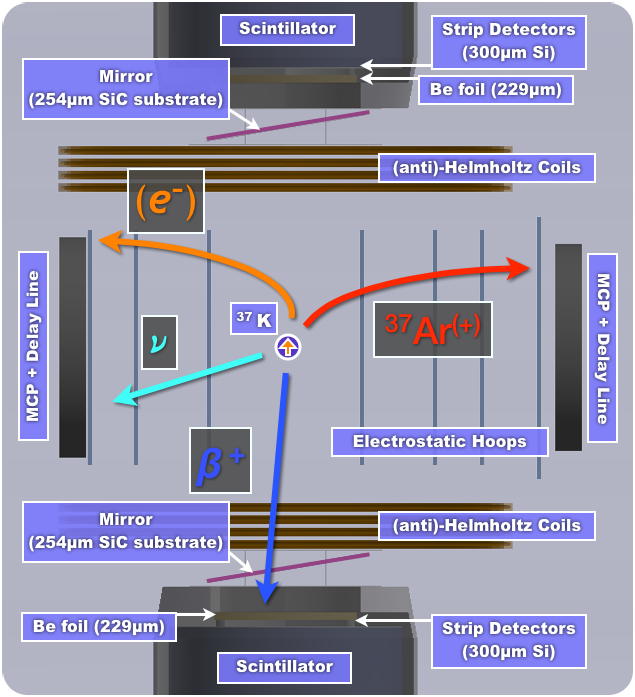
\includegraphics[width=.530\linewidth]{Figures/chamber_decayevent3.png}\label{chamber_decayevent} }
%	\hspace*{\fill}
%	\hfill
%	\hspace*{\fill}
%	\subfloat[Inside the TRINAT science chamber.  This photo is taken from the vantage point of one of the microchannel plates, looking into the chamber towards the second microchannel plate.  The current-carrying copper Helmholtz coils and two beta telescopes are visible at the top and bottom.  The metallic piece near the center is one of the electrostatic `hoops' used to generate an electric field within the chamber.  The hoop's central circular hole allows access to the microchannel plate, and the two elongated holes on the sides allow the MOT's trapping lasers to pass unimpeded at an angle of 45 degress `out of the page'.]	
%	{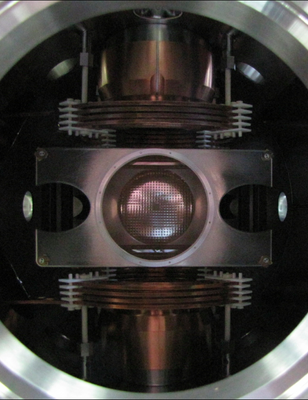
\includegraphics[width=.444\linewidth]{Figures/chamber_photo_2.png}}
%	\hspace*{\fill}%
%	\caption{The TRINAT detection chamber}	
%	\label{fig:thechamber}
%\end{figure}
%\clearpage
%\color{black}
%
%\subsection{Trapping}
%\label{trap}
%The Magneto-Optical Trap is a well-known technique from atomic physics, used to confine and cool neutral atoms~\cite{raabprentiss}.  The technique is used predominantly with alkalis due to their simple orbital electron structure, and is quite robust, so is appropriate for use with $^{37}\textrm{K}$.  Once set up, the trapping force is specific to the isotope for which the trap has been tuned, which makes it ideal for use in radioactive decay experiments, since the daughters are unaffected by the trapping forces keeping the parent confined.
%
%There are two primary components necessary for any MOT:  a laser, and a magnetic field.  The laser, which must be circularly polarized in the appropriate directions and tuned slightly to the red of an atomic resonance, is split into three perpendicular retroreflected beams, doppler cooling the atoms and (with the appropriate magnetic field) confining them in all three dimensions (see Figure~\ref{fig:mot}).  The TRINAT science chamber includes 6 `viewports' specifically designed to be used for the trapping laser.
%
%A MOT also requires a quadrupolar magnetic field, which we generate with two current-carrying anti-Helmholtz coils located within the vacuum chamber itself.  The coils themselves are hollow, and are cooled continuously by pumping temperature-controlled water through them.   
%
%One feature which makes our MOT unusual has been developed as a result of our need to rapidly cycle the MOT on and off -- that is, it is an ``AC-MOT''.  Rather than running the trap with one particular magnetic field and one set of laser polarizations to match, we run a sinusoidal AC current in the magnetic field coils, and so the sign and magnitude of the magnetic field alternate smoothly between two extrema, and the trapping laser polarizations are rapidly swapped to remain in sync with the field~\cite{harveymurray}\cite{thesis}.  See Figure~\ref{fig:acmot}.  
%
%\begin{figure}[ht]
%	\centering
%	\subfloat[Components of a magneto-optical trap, including current-carrying magnetic field coils and counterpropagating circularly polarized laser beams.]
%	{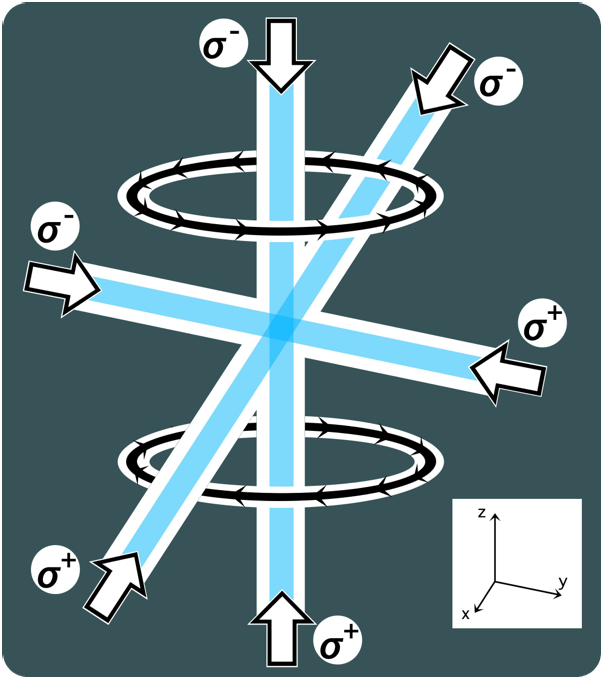
\includegraphics[width=.237\linewidth]{Figures/mot.png}\label{fig:mot} }
%	\hspace*{\fill}
%%	\hfill
%	\hspace*{\fill}
%	\subfloat[One cycle of trapping with the AC-MOT, followed by optical pumping to spin-polarize the atoms.  After atoms are transferred into the science chamber, this cycle is repeated 500 times before the next transfer.  The magnetic dipole field is created by running parallel (rather than anti-parallel as is needed for the MOT) currents through the two coils.]	
%	{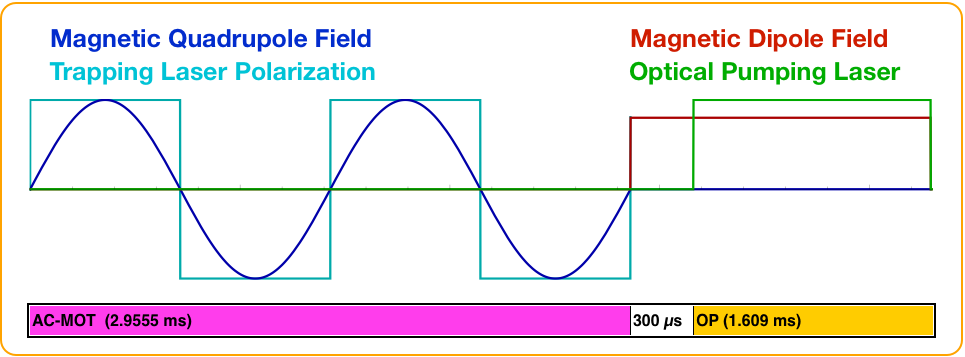
\includegraphics[width=.726\linewidth]{Figures/acmot.png}\label{fig:acmot} }
%	\caption{An alternating-current magneto-optical trap with a duty cycle optimized for producing polarized atoms}	
%	\label{fig:themot}
%\end{figure}
%
%The need to use an AC-MOT rather than a typical MOT has arisen as a direct result of our desire to optimally polarize our sample of atoms.  Polarization is incompatible with the non-uniform magnetic field used by a MOT, and rapidly shutting off the current used to produce the MOT's magnetic field produces eddy currents in the surrounding materials, which in turn produce their own non-uniform magnetic field in the region of interest.  The AC-MOT is developed as a way to ensure that the unavoidable eddy currents are behaving as we expect.  With an appropriate choice of shut-off phase, the current in the coils can be shut off when the overall magnetic field is already zero, so that no further eddy currents are induced.   

%{\color{cyan} (...) (something about why we need to run an AC-MOT.) }

%%%  Cut here?  %%%
%Note that because the atoms within a MOT can be treated as following a thermal distribution, some fraction of the fastest atoms continuously escape from the trap's potential well.  Even with the most carefully-tuned apparatus, the AC-MOT cannot quite match a similar standard MOT in terms of retaining atoms.  The TRINAT AC-MOT has a `trapping half-life' of around 6 seconds, and although that may not be particularly impressive by the standards of other MOTs, it is more than adequate for our purposes.  $^{37}\textrm{K}$ itself has a radioactive half-life of only 1.6 seconds \comment{(cite someone)}, so our dominant loss mechanism is radioactive decay rather than thermal escape. \comment{(Cut this whole paragraph?)}
%%%     %%%     %%%
%\clearpage

%


%\subsection{Optical Pumping}
%\label{op}
%We spin-polarize $^{37}\textrm{K}$ atoms within the trapping region by optical pumping~\cite{ben_OP}.  A circularly polarized laser is tuned to match the relevant atomic resonances, and is directed through the trapping region along the vertical axis in both directions.  When a photon is absorbed by an atom, the atom transitions to an excited state and its total angular momentum (electron spin + orbital + nuclear spin) along the vertical axis is incremented by one unit.  When the atom is de-excited a photon is emitted isotropically, 
%%\comment{(is it still isotropic when it's polarized?  I bet it's not.)}
%so it follows that if there are available states of higher and lower angular momentum, the \emph{average} change in the angular momentum projection is zero.  If the atom is not yet spin-polarized, it can absorb and re-emit another photon, following a biased random walk towards complete polarization.  
%
%In order to optimally polarize a sample of atoms by this method, it is necessary to have precise control over the magnetic field.  This is because absent other forces, a spin will undergo Larmor precession about the magnetic field lines.  In particular, the magnetic field must be aligned along the polarization axis (otherwise the tendency will be to actually depolarize the atoms), and it must be uniform in magnitude over the region of interest (otherwise its divergencelessness will result in the field also having a non-uniform direction, which results in a spatially-dependent depolarization mechanism).  Note that this type of magnetic field is not compatible with the MOT, which requires a quadrupolar magnetic field \emph{gradient}, and has necessitated our use of the AC-MOT as described in Subsection~\ref{trap}.


%\subsection{The Detectors}
%\label{detectors}
%\label{field}
%The beta detectors, located above and below the atom cloud along the axis of polarization (see Figure~\ref{chamber_decayevent}), are each the combination of a plastic scintillator and a set of silicon strip detectors.  Using all of the available information, these detectors are able to reconstruct the energy of an incident beta, as well as its hit position, and provide a timestamp for the hit's arrival.  Together the upper and lower beta detectors subtend approximately 1.4\% of the total solid angle as measured with respect to the cloud position. 
%
%It must be noted that the path between the cloud of trapped atoms and either beta detector is blocked by two objects:  a 254$\,\mu$m silicon carbide mirror (necessary for both trapping and optical pumping), and a 229$\,\mu$m beryllium foil (separating the UHV vacuum within the chamber from the outside world).  In order to minimize beta scattering and energy attenuation, these objects have had their materials selected to use the lightest nuclei with the desired material properties, and have been manufactured to be as thin as possible without compromising the experiment.  As the $^{37}\textrm{K} \rightarrow \,^{37}\textrm{\!Ar} + \beta^{+} + \nu_e$ decay proceess releases $Q=5.125$\,MeV of kinetic energy~\cite{Q_value}, the great majority of betas are energetic enough to punch through both obstacles without significant energy loss before being collected by the beta detectors.  
%
%On opposing sides of the chamber, and perpendicular to the axis of polarization, two stacks of $\sim$ 80\,mm diameter microchannel plates (MCPs) have been placed (see Figure~\ref{fig:thechamber}) as detectors, providing a time stamp when a particle is incident on their surfaces.  Behind each stack of MCPs there is a set of delay lines, which provide  position sensitivity for these detectors.   
%
%In order to make best use of these MCPs, we create an electric field in order to draw positively charged particles into one MCP, while drawing negatively charged electrons into the other MCP.  Seven electrostatic hoops have been placed within the chamber (see Figure~\ref{fig:thechamber}), and are connected to a series of high voltage power supplies.  See Sections~\ref{photoions} and~\ref{pos_recoils} for a discussion of what sort of charged particles we expect to observe in these detectors and how they are created.  
%  
%%\comment{(Say something about field uniformity?)}
%
%Scientific data has been collected at field strengths of 395 V/cm, 415 V/cm, and 535 V/cm.  It should be noted that these field strengths are too low to significantly perturb any but the least energetic of the (positively charged) betas from the decay process, and these low energy betas would already have been unable to reach the upper and lower beta detectors due to interactions with materials in the SiC mirror and Be foil vacuum seal.  
%


%\subsection{Cloud Measurements via Photoionization}
%\label{cloud}
%\label{photoions}
%In order to measure properties of the trapped $^{37}\textrm{K}$ cloud, a 10\,kHz pulsed laser at 355\,nm is directed towards the cloud.  These photons have sufficient energy to photoionize neutral $^{37}\textrm{K}$ from its excited atomic state, releasing 0.77\,eV of kinetic energy, but do not interact with ground state $^{37}\textrm{K}$ atoms.  The laser is of sufficiently low intensity that the great majority of excited state atoms are \emph{not} photoionized, so the technique is only very minimally destructive.  
%
%Because an electric field has been applied within this region (see Section~\ref{field}) the $^{37}\textrm{K}^+$ ions are immediately pulled into the detector on one side of the chamber, while the freed $e^-$ is pulled towards the detector on the opposite side of the chamber.  Because  $^{37}\textrm{K}^+$ is quite heavy relative to its initial energy, it can be treated as moving in a straight line directly to the detector, where its hit position on the microchannel plate is taken as a 2D projection of its position within the cloud.  Similarly, given a sufficient understanding of the electric field, the time difference between the laser pulse and the microchannel plate hit allows for a calculation of the ion's initial position along the third axis.  
%
%With this procedure, it is possible to produce a precise map of the cloud's position and size, both of which are necessary for the precision measurements of angular correlation parameters that are of interest to us here.  However, it also allows us to extract a third, slightly more subtle and significantly more important measurement:  the cloud's \emph{polarization}.
%
%The key to the polarization measurement is that only atoms in the excited atomic state can be photoionized.  While the MOT runs, atoms are constantly being pushed around and excited by the trapping lasers, so this period of time provides a lot of information for characterizing the trap size and position.  When the MOT is shut off, the atoms quickly return to their ground states and are no longer photoionized until the optical pumping beam is turned on.  As described in Section~\ref{op}, and in greater detail in~\cite{ben_OP}, the optical pumping process involves repeatedly exciting atoms from their ground states until the atoms finally cannot absorb any further angular momentum and remain in their fully-polarized (ground) state until they are perturbed.  Therefore, there is a sharp spike in excited-state atoms (and therefore photoions) when the optical pumping begins, and none once the cloud has been completely polarized.  The number of photoion events that occur once the sample has been maximally polarized, in comparison with the size and shape of the initial spike of photoions, provides a very precise characterization of the cloud's final polarization~\cite{ben_OP}.



%\comment{Photoions, the MCP, polarization stats, camera.}
%{\color{cyan} (...) }

%
\section{The Decay Process}
\label{decayprocess}
\label{pos_recoils}
% % %
The kinematics of nuclear $\beta^+$ decay are described by the following probability density function:
\bea
\label{jtw_pdf}
W(\langle I \rangle | E_\beta \hat{\Omega}_\beta \hat{\Omega}_\nu) 
&=& \left(\frac{1}{2\pi}\right)^{\!5} \!\! F\!\left( - Z, E_\beta \right)\, 
p_\beta E_\beta (E_0 - E_\beta)^2 \textrm{d}E_\beta \textrm{d}\hat{\Omega}_\beta \textrm{d}\hat{\Omega}_\nu \, \xi 
\left[ 1 + a_{\beta\nu} \frac{\vec{p}_\beta \cdot \vec{p}_\nu}{E_\beta E_\nu}
+ b_{\textrm{Fierz}} \frac{m_e}{E_\beta} 
\phantom{\frac{\left(\vec{p}_\beta\right)^2}{\vec{p}_\beta}} \!\!\!\! \right. \nonumber\\
%
&&\left. 
+ \, c_\textrm{align} \left( \frac{\frac{1}{3}\vec{p}_\beta \cdot \vec{p}_\nu - (\vec{p}_\beta \cdot \hat{j}) ( \vec{p}_\nu\cdot \hat{j} ) }{E_\beta E_\nu} \right) \!
 \left( \frac{I(I+1) - 3\langle (\vec{I}\cdot\hat{i})^2 \rangle}{I(2I-1)} \right) 
\right. \nonumber\\
%
&& \left. 
+ \frac{\langle \vec{I} \rangle}{I} \left( A_\beta\frac{\vec{p}_\beta}{E_\beta} + B_\nu \frac{\vec{p}_\nu}{E_\nu} + D_{\textrm{TR}} \frac{\vec{p}_\beta \times \vec{p}_\nu}{E_\beta E_\nu} \right)
\right],
\eea
where $\vec{I}$ is the nuclear spin-polarization, $F\!\left( - Z, E_\beta \right)$ is the Fermi function, 
and parameters $\xi$, $a_{\beta\nu}$, $ b_{\textrm{Fierz}}$, $c_\textrm{align}$, $A_\beta$, $B_\nu$, and $D_{\textrm{TR}}$ are functions that vary with the strengths of the vector, axial, scalar, and tensor couplings (constant throughout nature), as well as the Fermi and Gamow-Teller nuclear matrix elements (specific to the individual decay)~\cite{jtw}\cite{jtw_coulomb}.

%{\color{cyan} (...) }

The decay may be treated as a three-body problem in which the available kinetic energy is divided up between the beta, the neutrino, and the recoiling $^{37}\textrm{\!Ar}$ nucleus, and (of course) the total linear and angular momentum are conserved.  While the neutrino cannot be detected directly, its kinematics may be reconstructed from observations of the beta and the recoiling daughter nucleus.  By placing detectors above and below the decaying atom along the axis of its polarization, we are able to obtain information about the outgoing beta's energy and momentum, in the cases of interest to us, where it is emitted along (or close to) the axis of polarization.  

The recoiling $^{37}\textrm{\!Ar}$ nucleus is a bit trickier to work with, but the task is not impossible.  One useful feature of the $^{37}\textrm{K} \rightarrow \,^{37}\textrm{\!Ar}$ transition is that, in addition to the $\beta^+$ emitted in the decay itself, one or more \emph{orbital} electrons from the parent atom are typically lost.  In the majority of decay events
%\comment{(80\% of them?  Give a number.  Cite someone.  Dan's thesis?~\cite{dan_thesis}  Or Alexandre's talk from like 1999.)}, 
only one orbital electron is `shaken off' and so the daughter $^{37}\textrm{\!Ar}$ atom is electrically neutral~\cite{gorelov2000}\cite{dan_thesis}.  In the remaining cases, two or more orbital electrons are lost this way, and the daughter atom is positively charged.  If we apply an electric field perpendicular to the direction of polarization, these positively charged $^{37}\textrm{\!Ar}^{(+n)}$ ions may be collected into a detector, from which hit position and time of flight information may be extracted.  These shake-off electrons are emitted with an average energy of only $\sim$ 2\,eV
%very little kinetic energy ($\sim$ 2\,eV)
%\comment{(give a number.  2 eV?  I should check.  Also, do I cite one of John's talks here?)}, 
so to a very good approximation the other decay products are not perturbed by the presence of shake-off electrons.  

It should be noted that for the class of decays of greatest interest, where the beta and the neutrino emerge back-to-back along the polarization axis, the recoiling daughter nucleus will have zero momentum along the directions perpendicular to this axis, and on average less total energy than if the beta and neutrino were emitted in a parallel direction.  Henceforth, daughter nuclei from a back-to-back decay as shown in Figure~\ref{fig:rhc} will be described as `slow' recoils.  In terms of observables, this means that if the electric field is configured to point along one of the axes perpendicular to the polarization direction, then when the recoiling ion is swept away into a detector, the slow recoil's hit position should be exactly along the projection of the polarization axis.  Furthermore, the slow recoil's time of flight should be in the middle of the time of flight spectrum, since other recoils will be emitted with momentum towards or away from the detector.  

%Of course, in any real experiment, the number of decays emitted in exactly one set of directions will be a set of measure zero.  \comment{(say something about the limits taken as beta decay events approach the optimal set of angles.  Or just delete this paragraph because it's stupid.)}
% % %

%\section{Proposed Project}
%\label{project}
%Using $^{37}\textrm{K}$ beta decay data collected in June 2014, I intend to reconstruct the recoil momenta both along the polarization axis and perpendicular to it, such that when combined with energy and hit position from the beta detectors, each event's full kinematics may be reconstructed.  The spectra created by these events will be compared against a series of Geant4-based Monte Carlo simulations.  
%
%Matched template fitting will be used to compare the experimental data to the simulation, meaning that the implicit vector, axial, scalar, and tensor couplings within Eq.~\ref{jtw_pdf} will be allowed to float separately within the simulation, and a series of simulation ``templates'' will be produced, and each separately fit to the data.  The quality of each fit will be used to determine a ``best'' experimental value for both parameters, as well as the error inherent in the measurement.  
%
%%{\color{cyan} (...) }
%%\comment{See Figure~\ref{fig:Rslow_tof} ?}
%\begin{figure}[h!!t]
%	\centering
%	\includegraphics[width=.999\linewidth]
%	{Figures/Rslow_tof_squished.png}
%	\caption{Time-of-flight spectra for charged $^{37}\textrm{\!Ar}$ recoils at 535 V/cm, sorted by whether the $\beta$ was detected after emerging \emph{with} or \emph{against} the nuclear polarization direction, compared against a simulation using a uniform electric field.  	Recoils with zero initial momentum along the flight axis arrive in the center of the distribution for their charge state.  
%	}	
%	\label{fig:Rslow_tof}
%\end{figure}

%
\section{Current Status}
\label{status}
In June 2014, after several years of preparatory work beforehand (the author has been continuously involved with this project since 2010), approximately 7 days of beam time at TRIUMF was dedicated to the TRINAT $^{37}\textrm{K}$ beta decay experiment.  Approximately half of this data is suitable for use in this project.  During this period, approximately 10,000 atoms were held within the trap at any given time.  The cleaned spectra show around 50,000 polarized beta-recoil coincidence events in total, divided among measurements at three different electric field strengths (535 V/cm, 415 V/cm, 395 V/cm). 

%At the present time, analysis is underway.  The recoil MCP hit position data has been calibrated, and systematic effects in the trap position and size measurements are being considered.  The largest two remaining hurdles for the analysis both lie in improvements to the Monte Carlo.  

%The first challenge is to implement particle tracking within a \emph{non-uniform} electric field.  Using the true non-uniform electric field will shift the time-of-flight spectra overall by around 1\%, and is expected to change the \emph{shape} of spectra as well, since the deviation from uniformity changes significantly as a function of flight tragectory, and is greater the farther a particle ventures from the central axis.  This would affect the measured hit positions as well.  Taken together, the shape of the time-of-flight spectra (as in Figure~\ref{fig:Rslow_tof}) and the recoil hit position are critical to our reconstruction of the decay process, it is critical that we model them correctly.  

%The second challenge will be to allow our simulation to vary vector, axial, scalar, and tensor coupling constants separately while holding other physical parameters (such as the half-life and Fermi/Gamow-Teller ratio) constant.  This, too, will be absolutely critical to the analysis, and its implementation is likely to be non-trivial.

A fit to simulation has shown that the data that has already been collected has sufficient statistical power to measure the \emph{fractional} contribution of any polarized `new physics' beta decay parameter (ie right-handed, scalar, and tensor currents within the weak interaction) to a sensitivity of $\sim 2\%$ of its true value.  Systematic limitations are still being assessed.  
%Because previous measurements have already shown that any $(V-A)$, $S$, and $T$ terms within the Standard Model must be quite small~\cite{severijns_beck_cuncic_2006}\cite{severijns_cuncic_2011}, the present measurement is not likely to be able to add any new constraints to our understanding of Standard Model physics, and must instead be understood as complementary to previous measurements.
%Because previous measurements have 
%Quantifying this observable's sensitivity to physics beyond the Standard Model in comparison to previously measured constraints~\cite{severijns_beck_cuncic_2006}\cite{severijns_cuncic_2011} is work in progress.  



%Approximately of beamtime and several years of preparatory work beforehand, and its analysis is currently underway.  The statistical strength of our data is sufficient for a \comment{5\%?  (John said 5\%, but I don't really know how he calculated that...)} measurement to constrain right-handed weak interactions, however the systematic effects within the data have not yet been fully evaluated.  This constraint is far too weak to allo w for the discovery of a right-handed component of the nuclear weak force, and is likely also too weak to place any new constraints on its strength.  It could, at best, lend statistical strength to the constraints on right-handed currents that have already been observed.
%
%Unfortunately, due to beam scheduling and target creation procedures at TRIUMF, and because several components of the TRINAT science chamber have subsequently been removed and disassembled to prepare for future upgrades to the apparatus, it would be extremely difficult to collect any further data in a timely fashion.  

%\pagebreak       % JB says:   Appendix I  keep, it's excellent. It should be moved as is to Conclusions under "Future Experiment for the collaboration"! so people know you worked so hard on it!!

%\chapter[Fucking Duh]{Things that Should Be Very Fucking \mbox{Obvious}}
\label{fuckingduh}
%This section is not going to make it in to the final version, I hope, even if I really really need more pages.  Really, it's kind-of unfortunate that it gets included it in the drafts, but it's a pretty good place to store relevant information that I keep forgetting.

\section{The Center of Gravity}
It's what happens when you set $A = 0$ and $B = 0$.   That is all.

\section{Diagonalizing the Hamiltonian}
Given a Hermitian matrix $\hat{\Omega}$, there exists a unitary matrix $\hat{U}$ such that $\hat{U}^{\dagger}\hat{\Omega}\hat{U}$ is diagonalized.  Solving for this matrix $\hat{U}$ is, in this case, equivalent to solving the eigenvalue problem for $\hat{\Omega}$ \cite{shankar}.  As it turns out, $\hat{U}$ is the matrix of eigenvectors of $\hat{\Omega}$, by which I mean that the eigenvectors are column vectors, and they're all squished together to make $\hat{U}$.  It doesn't matter what order you put them in, but they probably have to be normalized.

Then, if 
\beq
\hat{\Omega}^{'} := \hat{U}^{\dagger}\hat{\Omega}\hat{U},
\eeq	
we find that $\hat{\Omega}^{'}$ is the diagonal matrix with its elements being the eigenvalues.  They're in the same order as the eigenvectors we squished together to make $\hat{U}$ previously.

Also, a unitary operator, $\hat{U}$ is one which satisfies:
\bea
\hat{U}\hat{U}^{\dagger} = \hat{U}^{\dagger}\hat{U}  = \undertilde{I}.
\eea

\section{Rotating Coordinates}
\label{rotating}
If by $\hat{\Omega}$ we really mean the Hamiltonian $\hat{H}$, and by $\hat{U}$ we really mean a coordinate change that takes us to rotating coordinates such that we can easily make a rotating wave approximation, we must take more things into account.  In particular, we find that our new rotating-coordinate Hamiltonian, $\tilde{H}$ is given by:
\beq
\tilde{H} = \hat{U}^{\dagger} \hat{H} \hat{U} - \hbar \hat{A}
\eeq
where
\beq
\hat{U} := e^{-i \hat{A} t}.  
\eeq
This additional term arises from our statement of the Schrodinger equation, 
\beq
\label{schrodingerpartial}
\hat{H} \ket{\psi} = i \hbar \frac{\partial}{\partial t} \ket{\psi}.
\eeq
In particular, note that~\ref{schrodingerpartial} includes only a partial derivative of the wavefunction.  I derive this result explicitly in Chapter~\ref{general_rotating}.  See also Ref.~\cite{budker_opticallypolarized}, pg.~195.
% See, for example, Ref.~\cite{opticallypolarizedatoms}, pg.~195.  

\section{Lifetimes and Half-Lifes}
Since different people use different notation to describe exponential decay of a physical quantity, it is useful to be able to relate two of the most common methods for describing the decay.  We begin with the rate equation,
\bea
\label{rateequation}
\frac{d N}{d t} &=& -\gamma\: N,
\eea
where it is clear that the ``rate" of decay must be $\gamma\: N$.  If we initially have $N_0$ of the quantity in question, then Eq.~\ref{rateequation} has as its solution
\bea
\label{rateequationsolution}
N(t) &=& N_0 \:e^{-\gamma\: t}.
\eea
Note that the physical interpretation of $\gamma$ is the ``linewidth''.  

We'll wish to convert $\gamma$ into other quantities of interest.  In particular, we can re-write the solution \ref{rateequationsolution} as
\bea
N(t) &=& N_0 \:e^{-t/\tau},
%&=& N_0 \left( \frac{1}{2} \right)^{t/t_{1/2}}.
\eea
where $\tau = 1/\gamma$ is referred to as the ``lifetime''.  Then, we find the half-life $t_{1/2}$ by enforcing the fact that it is the time at which the number of remaining atoms is equal to half of what was originally present.  Therefore, 
\bea
N(t_{1/2}) = N_0 e^{-t_{1/2} / \tau} &=& \frac{1}{2} N_0 \\ 
%\eea
%and
%\bea
e^{-t_{1/2} / \tau} &=&  1/2 \\ 
t_{1/2} / \tau &=& \ln(2).
\eea

Thus, we see that 
\bea
%\tau &=& 1/\gamma \\
t_{1/2} &=& \ln (2) \: \tau, 
\eea
where $\tau$ is the ``lifetime'' of the state, and $t_{1/2}$ is its ``half-life''.

%\section{Lifetimes and Half-Lifes}
%Since different people use different notation to describe exponential decay of a physical quantity, it is useful to be able to relate two of the most common methods for describing the decay.  We begin with the rate equation,
%\bea
%\label{rateequation}
%\frac{d N}{d t} &=& -\gamma\: N,
%\eea
%where it is clear that the ``rate" of decay must be $\gamma\: N$.  If we initially have $N_0$ of the quantity in question, then Eq.~\ref{rateequation} has as its solution
%\bea
%\label{rateequationsolution}
%N(t) &=& N_0 \:e^{-\gamma\: t}.
%\eea
%Note that the physical interpretation of $\gamma$ is the ``linewidth''.  
%
%We'll wish to convert $\gamma$ into other quantities of interest.  In particular, we can re-write the solution \ref{rateequationsolution} as
%\bea
%N(t) &=& N_0 \:e^{-t/\tau} \\
%&=& N_0 \left( \frac{1}{2} \right)^{t/t_{1/2}}.
%\eea
%Thus, we see that 
%\bea
%\tau &=& 1/\gamma \\
%t_{1/2} &=& \ln (2) \: \tau, 
%\eea
%where $\tau$ is the ``lifetime'' of the state, and $t_{1/2}$ is its ``half-life''.

\section{Reduced Matrix Elements}
% via http://quantummechanics.ucsd.edu/ph130a/130_notes/node426.html , which is nice but also I should find some other source if I ever use this for anything ever.
% Actually, see Shankar pg. 420.  But I still don't know what it *means*.
% Similarly for Sakurai pg. 239.
The Wigner-Eckart Theorem says, for vector operator $V^q$,
\beq
\langle \alpha ' j' m' | V^q | \alpha j m \rangle = \langle j' m' | j1 m q\rangle \langle \alpha ' j' \| V \|\alpha j \rangle .
\eeq
The point being that $\langle \alpha ' j' \| V \|\alpha j \rangle$ is the same for all $m$ and $q$.


\section{Doppler Cooling Limit}
Here it is!
\beq
k T_{\textrm{D}} = \frac{1}{2} \hbar \Gamma
\eeq

%\section{Order of Magnitude Estimates for Magnetic Perturbations}
%We'll optically pump our atoms with a laser tuned close to some resonant frequency.  Also, there might be transverse magnetic fields.  The Hamiltonian term for an atom in an electric field is:
%\beq
%\label{stark}
%\hat{H}_{\vec{E}} = -\vec{d} \cdot \vec{E}, 
%\eeq
%where
%\beq
%\vec{d} = \alpha \vec{E}, 
%\eeq
%and $\alpha$ is the ``atomic polarizability", which is different for different types of atoms.  We like to refer to this part of the Hamiltonian as the Stark Effect, and in fact, this is only the lowest-order (dipole) term of the perturbation.  For Hydrogen, $\alpha_{H} = 0.67 \times 10^{-24} \mathrm{cm}^3$, though I don't know where I got that number from originally, and should probably check on that.
%
%The term in the Hamiltonian for the interaction between the atom and the external magnetic field is given by:
%\beq
%\label{zeeman}
%\hat{H}_{\vec{B}} = - \vec{\mu} \cdot \vec{B}.
%\eeq
%We call that one the Zeeman Effect, and again this is only the lowest-order (dipole) term.
%
%As it turns out, those Hamiltonians are really made for constant, non-varying fields.  We probably have to do more things to find the Hamiltonians for the AC-Stark and AC-Zeeman effects.
%
%\emph{(Cite someone for this stuff.  Ref.~\cite{budker_opticallypolarized} pg.~63 is good for the DC Stark Effect.)}           % JB says:  Appendix J -> internal
% !TEX root = ../thesis_main.tex
%
%
%
%
%%%% --- * --- %%%%	
\chapter[SuperRatio]{Derivation of the $\bFierz$ Dependence of the Superratio Asymmetry}
\label{appendix:superratio}
\note[color=jb]{ Appendix KLM you have to pick what you want-- I hope that's Appendix K (that's this one!) -- and remove the rest as you say they're "old". Appendix K could be moved to the end of Experimental Methods because it's absolutely critical and helpful!! but if you want to reference it there and leave it as an Appendix, it's up to you.}


%Consider the following probability distribution for beta decay, which is equivalent to Eq.~(\ref{equation:integrated_jtw}).  %\aside{It's not just equivalent, it's literally identical.  }
Recall the integrated JTW probability distribution for outgoing beta particles from Eq.~(\ref{equation:integrated_jtw}):
\bea
	\textrm{d}^3 \Gamma ( \Ebeta, \mathbf{ \hat{\Omega}}_\beta ) \, \dEe \, \dOmegae
	&=& 
	\frac{2}{(2\pi)^4} \, \FF \, \pe \Ee (E_0 - \Ee)^2 \, \dEe \, \dOmegae \, \xi \nonumber\\ 
	&& \times \left[
		1 + \bFierz \frac{\m c^2}{\Ee} + 
		\A  
		\left(
			\frac{\vecJ}{J} \cdot \frac{\vecpe}{\Ee} 
		\right) 
	\right].
	\label{equation:integrated_jtw_in_superratiosection}
\eea
We note that the only angular dependence remaining in this equation is the dot product between the direction of beta emission and the direction of nuclear spin-polarization.  This allows us to pull out a further factor of $2\pi$ by choosing the axis of polarization as defining our coordinate system, and integrating over the ``$\phi_\beta$'' coordinate.  The result is a bit more friendly to work with:
%Integrating this distribution again over $\phi_\beta$, while reducing the
\bea
	\textrm{d}^2 \Gamma  ( \Ebeta, \theta ) \, \dEe \, \textrm{d} \theta %\, \dEe \, \dOmegae
	&=&
%	\frac{2}{(2\pi)^3} \, \FF \, \pe \Ee (E_0 - \Ee)^2 \, \dEe \, \dOmegae \, \xi \nonumber\\ 
%	&& \times \left[
%		1 + \bFierz \frac{\m c^2}{\Ee} + 
%		\A  
%		\left(
%			\frac{\vecJ}{J} \cdot \frac{\vecpe}{\Ee} 
%		\right) 
%	\right]
%	\\
%	&=&
	W(\Ebeta) \left[ 1 + \bFierz \frac{\m c^2}{\Ebeta} + \Abeta \, \frac{v_\beta }{c} |\vec{P}| \cos\theta  \right] \, \dEe \, \textrm{d} \theta , 
%\label{equation:integrated_jtw}
\eea
where $\theta$ is the angle between the beta emission direction and the polarization direction, and is the only angular dependence that remains.  Here, we have grouped the overall energy dependence into $W(\Ebeta)$, so that
\beq
W(\Ebeta) = \frac{2}{(2\pi)^3} \, \FF \, \pe \Ee (E_0 - \Ee)^2.
\eeq
\note{We could also use this with the Holstein formulation, at least some of it.  The point is, we can put *anything* that only depends on beta energy into $W(\Ebeta)$.  It doesn't matter, because it's already only integrable through numerical methods anyway -- so we can't possibly make it worse.}

In the TRINAT geometry with two polarization states (+/-) and two detectors (T/B) aligned along the axis of polarization, we are able to describe four different count rates, with different combinations of polarization states and detectors.  Thus, neglecting beta scattering effects, we have:
\bea
r_{\mathrm T+}(\Ebeta) &=& \varepsilon_{\mathrm T}(\Ebeta)\, \Omega_{\mathrm T} \, N_+ \left[1 + \bFierz \frac{\m c^2}{\Ebeta}  + \Abeta \, \frac{v}{c} |\vec{P}_+| \langle \cos\theta \rangle_{\mathrm T+} \right] \label{eq:r1} \\
r_{\mathrm B+}(\Ebeta) &=& \varepsilon_{\mathrm B}(\Ebeta)\, \Omega_{\mathrm B} \, N_+ \left[1 + \bFierz \frac{\m c^2}{\Ebeta}  + \Abeta \, \frac{v}{c} |\vec{P}_+| \langle \cos\theta \rangle_{\mathrm B+} \right] \label{eq:r2}\\
r_{\mathrm T-}(\Ebeta) &=& \varepsilon_{\mathrm T}(\Ebeta)\, \Omega_{\mathrm T} \, N_- \left[1 + \bFierz \frac{\m c^2}{\Ebeta}  + \Abeta \, \frac{v}{c} |\vec{P}_-| \langle \cos\theta \rangle_{\mathrm T-} \right] \label{eq:r3}\\
r_{\mathrm B-}(\Ebeta) &=& \varepsilon_{\mathrm B}(\Ebeta)\, \Omega_{\mathrm B} \, N_- \left[1 + \bFierz \frac{\m c^2}{\Ebeta}  + \Abeta \, \frac{v}{c} |\vec{P}_-| \langle \cos\theta \rangle_{\mathrm B-} \right],\label{eq:r4}
\eea
where $\varepsilon_{\mathrm T / \mathrm B}(\Ebeta)$ are the (top/bottom) detector efficiencies, $\Omega_{\mathrm T / \mathrm B}$ are the fractional solid angles for the (top/bottom) detector from the trap position, $N_{+/-}$ are the number of atoms trapped in each (+/-) polarization state, and $|\vec{P}_{+/-}|$ are the magnitudes of the polarization along the detector axis for each polarization state.  $\langle \cos\theta \rangle_{\mathrm T/ \mathrm B, +/-} $ is the average of $\cos\theta$ for \emph{observed} outgoing betas, for each detector and polarization state combination.  This latter term is approximately $\pm 1$ as a result of our detector geometry, but contains important sign information.  For a pointlike trap in the center of the chamber, 103.484 mm from either (DSSSD) detector, each of which is taken to be circular with a radius of 15.5 mm, we find that $\langle | \cos\theta | \rangle_{\mathrm T/ \mathrm B, +/-} \approx 0.994484$, and is the same for all four cases.
\aside{Not quite true.  Some strips are missing.}
% (or for $r=15.0$\,mm, we find that $\langle | \cos\theta | \rangle_{\mathrm T/ \mathrm B, +/-} \approx 0.994829$). 
\aside{This is only true if we neglect (back-)scatter.  This is not actually a good approximation.  But we have pretty good simulations to give us the real numbers, anyway. } Note that a horizontally displaced trap will decrease the magnitude of $\langle | \cos\theta | \rangle $, but as it is an expectation value of an absolute value, all four will remain equal to one another.  In the case of a vertically displaced trap, these four values will no longer all be equal, however it will still be the case that $\langle | \cos\theta | \rangle_{\mathrm T +} = \langle | \cos\theta | \rangle_{\mathrm T -}$, and $\langle | \cos\theta | \rangle_{\mathrm B+} = \langle | \cos\theta | \rangle_{\mathrm B -}$.  \aside{Is that definitely true, or is it only true to lowest order?}

In the case of the present experiment, we note that $|\vec{P}_+| = |\vec{P}_-|$ is correct to a high degree of precision.
				   % JB says:  "Appendix KLM you have to pick what you want-- I hope that's Appendix K-- and remove the rest as you say they're "old". Appendix K could be moved to the end of Experimental Methods because it's absolutely critical and helpful!! but if you want to reference it there and leave it as an Appendix, it's up to you."
\chapter[SuperRatio]{Derivation of the $\bFierz$ Dependence of the Superratio Asymmetry}

Consider, from JTW, the probability distribution for outgoing beta particles in terms of only the electron energy and direction w.r.t. parent nuclear polarization (other parameters have been integrated over).  We have
\bea
%P(\Ebeta) &=& W(\Ebeta) \left[ 1 + \bFierz \frac{mc^2}{\Ebeta} + \Abeta \, \frac{v}{c} |\vec{P}| \hat{P} \cdot \hat{\pbeta}  \right].
P(\Ebeta) &=& W(\Ebeta) \left[ 1 + \bFierz \frac{mc^2}{\Ebeta} + \Abeta \, \frac{v}{c} |\vec{P}| \cos\theta  \right].
\eea

In the TRINAT geometry with two polarization states (+/-) and two detectors (T/B), we are able to describe four different count rates, with different combinations of polarization states and detectors.  Thus, we have:
\bea
%\begin{subequations}
%\begin{align}
r_{\mathrm T+}(\Ebeta) &=& \varepsilon_{\mathrm T}(\Ebeta)\, \Omega_T \, N_+ \left[1 + \bFierz \frac{mc^2}{\Ebeta}  + \Abeta \, \frac{v}{c} |\vec{P}_+| \langle \cos\theta \rangle_{\mathrm T+} \right] \label{eq:r1} \\
r_{\mathrm B+}(\Ebeta) &=& \varepsilon_{\mathrm B}(\Ebeta)\, \Omega_B \, N_+ \left[1 + \bFierz \frac{mc^2}{\Ebeta}  + \Abeta \, \frac{v}{c} |\vec{P}_+| \langle \cos\theta \rangle_{\mathrm B+} \right] \label{eq:r2}\\
r_{\mathrm T-}(\Ebeta) &=& \varepsilon_{\mathrm T}(\Ebeta)\, \Omega_T \, N_- \left[1 + \bFierz \frac{mc^2}{\Ebeta}  + \Abeta \, \frac{v}{c} |\vec{P}_-| \langle \cos\theta \rangle_{\mathrm T-} \right] \label{eq:r3}\\
r_{\mathrm B-}(\Ebeta) &=& \varepsilon_{\mathrm B}(\Ebeta)\, \Omega_B \, N_- \left[1 + \bFierz \frac{mc^2}{\Ebeta}  + \Abeta \, \frac{v}{c} |\vec{P}_-| \langle \cos\theta \rangle_{\mathrm B-} \right],\label{eq:r4}
%\end{align}
%\end{subequations}
\eea
where $\varepsilon_{\mathrm T / \mathrm B}(\Ebeta)$ are the (top/bottom) detector efficiencies, $\Omega_{\mathrm T / \mathrm B}$ are the fractional solid angles for the (top/bottom) detector from the trap position, $N_{+/-}$ are the number of atoms trapped in each (+/-) polarization state, and $|\vec{P}_{+/-}|$ are the magnitudes of the polarization along the detector axis for each polarization state.  $\langle \cos\theta \rangle_{\mathrm T/ \mathrm B, +/-} $ is the average of $\cos\theta$ for \emph{observed} outgoing betas, for each detector and polarization state combination.  This latter term is approximately $\pm 1$, and contains important sign information.  For a pointlike trap in the center of the chamber, 103.484 mm from either (DSSSD) detector, each of which is taken to be circular with a radius of 15.5 mm, we find that $\langle | \cos\theta | \rangle_{\mathrm T/ \mathrm B, +/-} \approx 0.994484$, and is the same for all four cases (or for $r=15.0$\,mm, we find that $\langle | \cos\theta | \rangle_{\mathrm T/ \mathrm B, +/-} \approx 0.994829$). Note that a horizontally displaced trap will decrease the magnitude of $\langle | \cos\theta | \rangle $, but all four values will remain equal to one another.  In the case of a vertically displaced trap, these four values will no longer all be equal, however it will still be the case that $\langle | \cos\theta | \rangle_{\mathrm T +} = \langle | \cos\theta | \rangle_{\mathrm T -}$, and $\langle | \cos\theta | \rangle_{\mathrm B+} = \langle | \cos\theta | \rangle_{\mathrm B -}$.

For simplicity, we will henceforth assume that the trap is vertically centered, and take $|\vec{P}_+| = |\vec{P}_-|$.  We also define the following:
\bea
A^\prime &=& A^\prime(\Ebeta) \;\; \equiv \;\; \Abeta \, \frac{v}{c} \, |\vec{P}| \, \langle | \cos\theta | \rangle \\
b^\prime &=& b^\prime(\Ebeta) \;\; \equiv \;\; \bFierz \frac{mc^2}{\Ebeta},
\eea
and choose a coordinate system in which the + polarization state is, in some sense, `pointing up' toward the top detector, such that
\bea
\langle \cos\theta \rangle_{\mathrm T +} &\approx& +1 \\
\langle \cos\theta \rangle_{\mathrm B +} &\approx& -1 \\
\langle \cos\theta \rangle_{\mathrm T -} &\approx& -1 \\
\langle \cos\theta \rangle_{\mathrm B -} &\approx& +1.
\eea
This allows us to rewrite the four count rates in simplified notation, as: 
\bea
r_{\mathrm T+} &=& \varepsilon_{\mathrm T}N_+ \left(1 + b^\prime  + A^\prime \right) \\
r_{\mathrm B+} &=& \varepsilon_{\mathrm B}N_+ \left(1 + b^\prime  - A^\prime \right) \\
r_{\mathrm T-} &=& \varepsilon_{\mathrm T}N_- \left(1 + b^\prime  - A^\prime \right) \\
r_{\mathrm B-} &=& \varepsilon_{\mathrm B}N_- \left(1 + b^\prime  + A^\prime \right).
\eea
We further define the `superratio', $s$, to be:
\bea
s = \frac{ r_{\mathrm T-}\, r_{\mathrm B+} }{ r_{\mathrm T+}\, r_{\mathrm B-} }.
\eea
We are now in a position to define the `superratio asymmetry', $A_{\mathrm{super}}$, as
\bea
A_{\mathrm{super}} &=& A_{\mathrm{super}}(\Ebeta) \;\; \equiv \;\; \frac{1-\sqrt{s}}{1+\sqrt{s}}.
\eea
This is explicitly an experimental quantity that is measured directly by the above combination of count rates.  


Writing the superratio out explicitly in terms of $A^\prime$ and $b^\prime$, factors of $\varepsilon_{\mathrm T / \mathrm B}$ and $N_{+/-}$ cancel out entirely, and we find that
\bea
s &=& \frac{(1+b^\prime - A^\prime)^2}{(1+b^\prime+A^\prime)^2 }.
\eea
From here it is immediately clear that in absence of other corrections (\emph{e.g.} backscattering, unpolarized background, ...), if $b^\prime = 0$ it follows that $A_{\mathrm{super}} = A^\prime$.  In the case where $b^\prime \neq 0$, we find that 
\bea
A_{\mathrm{super}} &=& \frac{A^\prime}{1+b^\prime} \\
&\approx&  A^\prime \, (1 - b^\prime + {b^{\prime}}^2),
\eea
where we have utilized the assumption that $b^\prime \ll 1$.
Thus, 
\bea
A_{\mathrm{super}} &\approx& \Abeta \, \frac{v}{c} \, |\vec{P}| \, \langle | \cos\theta | \rangle - \Abeta \, \frac{v}{c} \, |\vec{P}| \, \langle | \cos\theta | \rangle \left( \bFierz \frac{mc^2}{\Ebeta}\right) + \Abeta \, \frac{v}{c} \, |\vec{P}| \, \langle | \cos\theta | \rangle \left(\bFierz \frac{mc^2}{\Ebeta}\right)^{\!\!2}.
\eea

%%% -- %%% -- %%% -- %%% -- %%% -- %%% -- %%% -- %%%










%%% -- %%% -- %%% -- %%% -- %%% -- %%% -- %%% -- %%%
\chapter[Super Corrections]{Some Corrections to the Superratio Stuff}
We consider further modifications to the rates described in Eqs.~(\ref{eq:r1}-\ref{eq:r4}).  In particular, we consider the effect of %a background signal on the two detectors, 
non-identical polarization magnitudes for the two polarization states and a trap displaced from the center.

We define for the polarization states:
\bea
P &\equiv& \frac{1}{2}\left(|\vec{P}_+| + |\vec{P}_+|\right) \\
\Delta P &\equiv& \frac{1}{2} \left(|\vec{P}_+| - |\vec{P}_+|\right)
\eea
and immediately find that
\bea
|\vec{P}_+| &=& P + \Delta P \\
|\vec{P}_-| &=& P - \Delta P.
\eea
Further, we also define:
\bea
\langle |\cos\theta | \rangle_T &\equiv& \langle |\cos\theta | \rangle_{\mathrm T+} \, = \, \langle |\cos\theta | \rangle_{\mathrm T-} \\
\langle |\cos\theta | \rangle_B &\equiv& \langle |\cos\theta | \rangle_{\mathrm B+} \, = \, \langle |\cos\theta | \rangle_{\mathrm B-},
\eea
%which is still true for a trap displaced from the center in any direction.  
and
\bea
\langle |\cos\theta | \rangle &\equiv& \frac{1}{2} \left( \phantom{2_2^2}\!\!\!\! \langle |\cos\theta | \rangle_T + \langle |\cos\theta | \rangle_B \, \right)\\
\Delta \langle |\cos\theta | \rangle &\equiv& \frac{1}{2} \left( \phantom{2_2^2}\!\!\!\! \langle |\cos\theta | \rangle_T - \langle |\cos\theta | \rangle_B \, \right).
\eea
It immediately follows that 
\bea
\langle |\cos\theta | \rangle_{\mathrm T} \, &=&\, \langle |\cos\theta | \rangle \, + \, \Delta \langle |\cos\theta | \rangle  \\
\langle |\cos\theta | \rangle_{\mathrm B} \, &=&\, \langle |\cos\theta | \rangle \, - \, \Delta \langle |\cos\theta | \rangle.
\eea
%For simplicity, we also will use
%\bea
%A^{\prime\prime} = A_\beta \, \frac{v}{c}.
%\eea

With this new set of variables defined, we can re-write Eqs.~(\ref{eq:r1}-\ref{eq:r4}) as
\bea
r_{\mathrm T+}(\Ebeta) &=& \varepsilon_{\mathrm T}(\Ebeta)\, N_+ \left[1 + b^\prime  + (A_\beta \frac{v}{c}) (P + \Delta P) \left( \phantom{2_2^2}\!\!\!\! \langle |\cos\theta | \rangle + \Delta \langle | \cos\theta | \rangle \, \right) \right] \\
r_{\mathrm B+}(\Ebeta) &=& \varepsilon_{\mathrm B}(\Ebeta)\, N_+ \left[1 + b^\prime  - (A_\beta \frac{v}{c}) (P + \Delta P) \left( \phantom{2_2^2}\!\!\!\! \langle |\cos\theta | \rangle - \Delta \langle | \cos\theta | \rangle \, \right) \right] \\
r_{\mathrm T-}(\Ebeta) &=& \varepsilon_{\mathrm T}(\Ebeta)\, N_- \left[1 + b^\prime  - (A_\beta \frac{v}{c}) (P - \Delta P) \left( \phantom{2_2^2}\!\!\!\! \langle |\cos\theta | \rangle + \Delta \langle | \cos\theta | \rangle \, \right) \right] \\
r_{\mathrm B-}(\Ebeta) &=& \varepsilon_{\mathrm B}(\Ebeta)\, N_- \left[1 + b^\prime  + (A_\beta \frac{v}{c}) (P - \Delta P) \left( \phantom{2_2^2}\!\!\!\! \langle |\cos\theta | \rangle - \Delta \langle | \cos\theta | \rangle \, \right) \right], 
\eea
and the superratio becomes
\bea
s &=& \frac{ \left( \phantom{\frac{2_2}{2}}\!\!\!\! 
1+b^\prime - (A_\beta \frac{v}{c})(P - \Delta P)\left( \phantom{2_2^2}\!\!\!\! \langle |\cos\theta | \rangle + \Delta \langle | \cos\theta | \rangle \, \right) \right) 
\left( \phantom{\frac{2_2}{2}}\!\!\!\! 
1+b^\prime - (A_\beta \frac{v}{c})(P + \Delta P)\left( \phantom{2_2^2}\!\!\!\! \langle |\cos\theta | \rangle - \Delta \langle | \cos\theta | \rangle \, \right) \right) 
}{ 
\left( \phantom{\frac{2_2}{2}}\!\!\!\!
1+b^\prime + (A_\beta \frac{v}{c})(P + \Delta P)\left( \phantom{2_2^2}\!\!\!\! \langle |\cos\theta | \rangle + \Delta \langle | \cos\theta | \rangle \, \right) \right) 
\left( \phantom{\frac{2_2}{2}}\!\!\!\! 
1+b^\prime + (A_\beta \frac{v}{c})(P - \Delta P)\left( \phantom{2_2^2}\!\!\!\! \langle |\cos\theta | \rangle - \Delta \langle | \cos\theta | \rangle \, \right) \right)},
\nonumber \\
\eea
where $\varepsilon_{\mathrm T / \mathrm B}$ and $N_{+/-}$ still completely cancel out.  After a bit of algebra, this simplifies to:
\bea
s &=& \frac{ 
%\left[ 
\left(\phantom{2_2^2}\!\!\!\! 
1+b^\prime - A^\prime + A_\beta \frac{v}{c} \Delta P \, \Delta \langle | \cos\theta | \rangle 
\right)^2 
- 
(A_\beta \frac{v}{c})^2 \left(\phantom{2_2^2}\!\!\!\!
\Delta P \langle | \cos\theta | \rangle - P \Delta\langle | \cos\theta |\rangle
\right)^2 
%\right] 
}{ 
%\left[ 
\left( \phantom{2_2^2}\!\!\!\! 
1+b^\prime + A^\prime + A_\beta \frac{v}{c} \Delta P \, \Delta \langle | \cos\theta | \rangle 
\right)^2 
- 
(A_\beta \frac{v}{c})^2 \left(\phantom{2_2^2}\!\!\!\! 
\Delta P \langle | \cos\theta | \rangle + P \Delta\langle | \cos\theta |\rangle
\right)^2 
%\right] 
}, \label{eq:simplifiedcorrectedsuperratio}
\eea
Note that in the superratio $\Delta P$ and $\Delta \langle |\cos\theta|\rangle$ have cancelled out to first order, and the remaining dependencies are quadratic only.  Eq.~(\ref{eq:simplifiedcorrectedsuperratio}) is exact, but still a huge enough expression to be pretty unweildy to work with.  Let's introduce some shorthand notation to make this less painful:  
\bea
A^{\prime\prime} &:=& A_\beta \frac{v}{c} \\ 
c &:=& \langle | \cos\theta | \rangle \\
\Delta c &:=& \Delta \langle | \cos\theta | \rangle \\ 
%r_0^+ &:=& 1+b^\prime + A^\prime \\ 
%r_0^- &:=& 1+b^\prime - A^\prime \\
%r_0 &:=& 1+b^\prime \\
r^\prime &:=& 1+b^\prime + A_\beta \frac{v}{c} \, \Delta P \, \Delta \langle | \cos\theta | \rangle
\eea
In this notation, we find that
\bea
s &=& \frac{ 
\left(\vphantom{2_2^2} 
%r_0 - A^\prime + A^{\prime\prime} \, \Delta P \, \Delta c
r^\prime - A^\prime
\right)^2 
- 
(A^{\prime\prime})^2 \left( \vphantom{2_2^2}
\Delta P \, c - P \, \Delta c
\right)^2 
}{ 
\left( \vphantom{2_2^2}
%r_0 + A^\prime + A^{\prime\prime} \, \Delta P \, \Delta c 
r^\prime + A^\prime 
\right)^2 
- 
(A^{\prime\prime})^2 \left( \vphantom{2_2^2} 
\Delta P \,c + P \, \Delta c
\right)^2 
},
\eea
which hurts a lot less to look at.  Then, the superratio asymmetry is
\bea
A_{\mathrm{super}} &=& \frac{
1 - \sqrt{ 
\frac{ 
\left(\vphantom{2_2^2} 
%r_0 - A^\prime + A^{\prime\prime} \, \Delta P \, \Delta c
r^\prime - A^\prime
\right)^2 
- 
(A^{\prime\prime})^2 \left( \vphantom{2_2^2}
\Delta P \, c - P \, \Delta c
\right)^2 
}{ 
\left( \vphantom{2_2^2}
%r_0 + A^\prime + A^{\prime\prime} \, \Delta P \, \Delta c 
r^\prime + A^\prime 
\right)^2 
- 
(A^{\prime\prime})^2 \left( \vphantom{2_2^2} 
\Delta P \,c + P \, \Delta c
\right)^2 
}
}
}{
1 + \sqrt{ 
\frac{ 
\left(\vphantom{2_2^2} 
r^\prime - A^\prime
\right)^2 
- 
(A^{\prime\prime})^2 \left( \vphantom{2_2^2}
\Delta P \, c - P \, \Delta c
\right)^2 
}{ 
\left( \vphantom{2_2^2}
r^\prime + A^\prime 
\right)^2 
- 
(A^{\prime\prime})^2 \left( \vphantom{2_2^2} 
\Delta P \,c + P \, \Delta c
\right)^2 
}
}
} \\
&=&
\frac{ \left[
\sqrt{\left( \vphantom{2_2^2}
r^\prime + A^\prime 
\right)^2 
- 
(A^{\prime\prime})^2 \left( \vphantom{2_2^2} 
\Delta P \,c + P \, \Delta c
\right)^2 
} - \sqrt{\left( \vphantom{2_2^2} 
r^\prime - A^\prime \right)^2 
- 
(A^{\prime\prime})^2 \left( \vphantom{2_2^2}
\Delta P \, c - P \, \Delta c \right)^2} \right]^2
}{
%\sqrt{ 
\left[ \left( \vphantom{2_2^2} 
r^\prime + A^\prime \right)^2 
- 
(A^{\prime\prime})^2 \left( \vphantom{2_2^2} 
\Delta P \,c + P \, \Delta c \right)^2 \right]
%}
 - 
%\sqrt{ 
\left[ \left(\vphantom{2_2^2} 
r^\prime - A^\prime \right)^2 
- 
(A^{\prime\prime})^2 \left( \vphantom{2_2^2}
\Delta P \, c - P \, \Delta c
\right)^2 \right] 
%}
} \\
&=&
\frac{%\mathrm{numerator}
\left(
\begin{array}{@{}c@{}}
2\left[  \vphantom{\sqrt{2}_2^2}
( r^\prime )^2 + (A^\prime)^2 - (A^{\prime\prime})^2\left( (P\,\Delta c)^2 + (\Delta P \, c)^2 \right)
\right] 
\\
- 2\left[ \left( \vphantom{2_2^2}
r^\prime + A^\prime 
\right)^2 
- 
(A^{\prime\prime})^2 \left( \vphantom{2_2^2} 
\Delta P \,c + P \, \Delta c
\right)^2 \right]^{1/2}
\left[ \left( \vphantom{2_2^2} 
r^\prime - A^\prime \right)^2 
- 
(A^{\prime\prime})^2 \left( \vphantom{2_2^2}
\Delta P \, c - P \, \Delta c \right)^2 \right]^{1/2}
\end{array} 
\right)
}{
4\left[ \vphantom{\sqrt{2}_2^2}
( r^\prime \, A^\prime )  - (A^{\prime\prime})^2 \left( P \, c \, \Delta P \, \Delta c \right) 
\right]
}
\eea


%Then (multiplying $\Asuper$ by factors of one), 
%\bea
%A_{\mathrm{super}} &=& \frac{ \left(\phantom{\frac{1^1}{1^1}}\!\!\!\!\! 
%\begin{array}{@{}c@{}}
%\phantom{-} \left[ \left( \phantom{2_2^2}\!\!\!\! 
%1+b^\prime + A^\prime + A_\beta \frac{v}{c} \Delta P \, \Delta \langle | \cos\theta | \rangle 
%\right)^2 
% - (A_\beta \frac{v}{c})^2 \left(\phantom{2_2^2}\!\!\!\! 
%\Delta P \langle | \cos\theta | \rangle + P \Delta\langle | \cos\theta |\rangle
%\right)^2  \right]^{1/2}  
%\\
%- \left[ \left(\phantom{2_2^2}\!\!\!\! 
%1+b^\prime - A^\prime + A_\beta \frac{v}{c} \Delta P \, \Delta \langle | \cos\theta | \rangle 
%\right)^2 
%- 
%(A_\beta \frac{v}{c})^2 \left(\phantom{2_2^2}\!\!\!\!
%\Delta P \langle | \cos\theta | \rangle - P \Delta\langle | \cos\theta |\rangle
%\right)^2 
% \right]^{1/2} 
%\end{array}
%\right)^2 
%}{ 
%\left( \begin{array}{@{}c@{}} \phantom{+} 
%\left[  \left( \phantom{2_2^2}\!\!\!\! 
%1+b^\prime + A^\prime + A_\beta \frac{v}{c} \Delta P \, \Delta \langle | \cos\theta | \rangle 
%\right)^2 
% - (A_\beta \frac{v}{c})^2 \left(\phantom{2_2^2}\!\!\!\! 
%\Delta P \langle | \cos\theta | \rangle + P \Delta\langle | \cos\theta |\rangle
%\right)^2   \right] 
%\;
%\\[0.6em]
%+ \left[ \left(\phantom{2_2^2}\!\!\!\! 
%1+b^\prime - A^\prime + A_\beta \frac{v}{c} \Delta P \, \Delta \langle | \cos\theta | \rangle 
%\right)^2 
%- 
%(A_\beta \frac{v}{c})^2 \left(\phantom{2_2^2}\!\!\!\!
%\Delta P \langle | \cos\theta | \rangle - P \Delta\langle | \cos\theta |\rangle
%\right)^2 
%\right] \;
%\end{array}
%\right)
%}, 
%\nonumber \\
%\eea
%which is clearly way too huge for me to have either written or typed out without making a mistake somewhere.  Still, the only thing to be done at this point is to expand it all out and make the expression even larger.  



%\bea
%r_{\mathrm T+}(\Ebeta) &=& \varepsilon_{\mathrm T}(\Ebeta)\, N_+ \left[1 + \bFierz \frac{mc^2}{\Ebeta}  + \Abeta \, \frac{v}{c} (P + \Delta P) \left( \phantom{2_2^2}\!\!\!\! \langle |\cos\theta | \rangle  +  \Delta \langle |\cos\theta | \rangle \, \right) \right]  + R_{\mathrm T}(\Ebeta) \\
%r_{\mathrm B+}(\Ebeta) &=& \varepsilon_{\mathrm B}(\Ebeta)\, N_+ \left[1 + \bFierz \frac{mc^2}{\Ebeta}  - \Abeta \, \frac{v}{c} (P + \Delta P) \left( \phantom{2_2^2}\!\!\!\! \langle |\cos\theta | \rangle - \Delta \langle |\cos\theta | \rangle \, \right) \right] + R_{\mathrm B}(\Ebeta)  \\
%r_{\mathrm T-}(\Ebeta) &=& \varepsilon_{\mathrm T}(\Ebeta)\, N_- \left[1 + \bFierz \frac{mc^2}{\Ebeta}  - \Abeta \, \frac{v}{c} (P - \Delta P) \left( \phantom{2_2^2}\!\!\!\! \langle |\cos\theta | \rangle +  \Delta \langle |\cos\theta | \rangle \, \right) \right] + R_{\mathrm T}(\Ebeta)  \\
%r_{\mathrm B-}(\Ebeta) &=& \varepsilon_{\mathrm B}(\Ebeta)\, N_- \left[1 + \bFierz \frac{mc^2}{\Ebeta}  + \Abeta \, \frac{v}{c} (P - \Delta P) \left( \phantom{2_2^2}\!\!\!\! \langle |\cos\theta | \rangle - \Delta \langle |\cos\theta | \rangle \, \right) \right] + R_{\mathrm B}(\Ebeta), 
%\eea
%where we have also introduced the additional energy-dependent background rates $R_{\mathrm T / \mathrm B}$, which are unique to each detector.











%